\documentclass{article}
\usepackage{amssymb}
\usepackage{amsthm}
\usepackage{amsmath}

% PAGE DIMENSION
\usepackage{geometry}

% BIBLIOGRAPHY
\usepackage{natbib}
\usepackage{bibentry} % inline refereces

% ENCODING, LANGUAGE
\usepackage[english]{babel}
\usepackage[utf8]{inputenc}

% GRAPHICS
\usepackage{subfig}
\usepackage{graphicx}

% HYPERTEXT, SOURCE CODE SPECIALS
\usepackage[unicode]{hyperref}
\usepackage[active]{srcltx} % use TeX-souce-specials-mode

% SYMBOLS, FONTS
\usepackage{mathbbol}
\usepackage{bm} % sophisticated \boldsymbol
%\usepackage{stmaryrd}
\usepackage{MnSymbol} % \lsem, \rsem, tensor product :
\usepackage{gensymb}
\usepackage{physics}
\usepackage{eurosym}

% UNITS, TYPESETTING TENSORS
\usepackage{units}
\usepackage{tensor}
\usepackage{accents}

% COMPACT LIST ENVIRONMENT
\usepackage{enumitem}

% LINE NUMBERS
\usepackage{lineno}

\usepackage{multicol}

% SELECTIVELY INCLUDE/EXCLUDE PARTS OF TEXT
\usepackage{comment}

% FLOAT BARRIER
\usepackage{placeins}

%\makeatletter
% \@ifpackageloaded{tensor}% tensor is a package for a better typesetting of tensors
% {
% \renewcommand{\tnsr@Aux}[3][]{%
% \mathpalette{\tnsr@Plt{#1}{#3}}{\mathrm #2}%
% \tnsr@Wrn
% }%\tnsr@Aux
% }{%
% \relax%
% }
% \makeatother


\theoremstyle{definition}
\newtheorem{definition}{Definition}
\newtheorem*{example}{Example}

\theoremstyle{plain}
\newtheorem{lemma}{Lemma}
\newtheorem{theorem}{Theorem}

\theoremstyle{remark}
\newtheorem*{remark}{Remark}

% operators
\DeclareMathOperator{\Sym}{Sym}
\DeclareMathOperator{\signum}{sign}
\DeclareMathOperator{\supp}{supp}
\DeclareMathOperator{\diam}{diam}
\DeclareMathOperator{\cof}{cof} % cofactor
\DeclareMathOperator{\residue}{res}
\DeclareMathOperator{\ad}{ad} % adjoint ad_X (Y) = [X,Y]  
\DeclareMathOperator{\dist}{dist} % distance in a metric space

% Load xparse (if not already loaded)
\usepackage{xparse}

% Continuous functions


\newcommand{\CkSet}[2]{%
	\ensuremath{\text{C}^{#1}\!\,\left(#2 \right)}}%

\newcommand{\CinfSet}[1]{%
	\ensuremath{\text{C}^{\infty}\!\,\left(#1 \right)}}%

\newcommand{\DSet}[1]{%
	\ensuremath{\mathcal{D}\!\,\left(#1 \right)}}%

\newcommand{\CklSet}[3]{%
	\ensuremath{\text{C}^{\!\, \,#1,#2}\!\,\left(#3 \right)}}%

\newcommand{\Ckl}[2]{%
\ensuremath{\text{C}^{\!\,\, #1,#2}}}%



%%%%%%%%%%%%%%%%%%%%%%%%%%%%%%%%%%%%%%%%%%%%%%%
% Lebesgue Spaces and Their Norms
%%%%%%%%%%%%%%%%%%%%%%%%%%%%%%%%%%%%%%%%%%%%%%%

% Generic Lebesgue space on a set.
\DeclareDocumentCommand{\LpSet}{ o m }{%
	\ensuremath{\text{L}_{\IfNoValueTF{#1}{\text{p}}{#1}}\!\left( #2 \right)}%
}


\newcommand{\LinfSet}[1]{%
	\ensuremath{\text{L}_{\infty}\!\,\left(#1 \right)}}%


% Norm in a Lebesgue space on a set.
\DeclareDocumentCommand{\NormLpSet}{ O{p} m m }{%
	\ensuremath{\norm{#2}_{\text{L}_{\IfNoValueTF{#1}{\text{p}}{#1}}\!\left( #3 \right)}}%
}

%%%%%%%%%%%%%%%%%%%%%%%%%%%%%%%%%%%%%%%%%%%%%%%
% Lebesgue-Bochner Spaces and Their Norms
%%%%%%%%%%%%%%%%%%%%%%%%%%%%%%%%%%%%%%%%%%%%%%%

%Generic Lebesgue - Bochner space on a set.
\newcommand{\LpIntX}[4]{%
	\ensuremath{\text{L}_{\text{#1}}\!\,\Bigl( (#2,#3);#4 \Bigr)}%
}

\newcommand{\LinfIntX}[3]{%
	\ensuremath{\text{L}_{\infty}\!\,\Bigl( (#1,#2);#3 \Bigr)}%
}

% Norm in a Lebesgue space on a set.
\newcommand{\NormLpIntX}[5]{%
	\ensuremath{\norm{#1}_{\text{L}_{\text{#2}}\!\,\left( (#3,#4);#5 \right)}}%
}

\newcommand{\NormLinfIntX}[4]{%
	\ensuremath{\norm{#1}_{\text{L}_{\infty}\!\,\left( (#2,#3);#4 \right)}}%
}


%%%%%%%%%%%%%%%%%%%%%%%%%%%%%%%%%%%%%%%%%%%%%%%
% Sobolev Spaces and Their Norms
%%%%%%%%%%%%%%%%%%%%%%%%%%%%%%%%%%%%%%%%%%%%%%%

% Generic Sobolev space on a set.
\DeclareDocumentCommand{\WkpSet}{ o o m }{%
	\ensuremath{\text{W}^{\IfNoValueTF{#1}{\text{k}}{#1},\IfNoValueTF{#2}{\text{p}}{#2}}\!\left( #3 \right)}%
}


% Sobolev space with zero boundary conditions on a set.
\DeclareDocumentCommand{\WkpzeroSet}{ o o m }{%
	\ensuremath{\text{W}^{\IfNoValueTF{#1}{\text{k}}{#1},\IfNoValueTF{#2}{\text{p}}{#2}}_0\!\left( #3 \right)}%
}

% Norm in a Sobolev space on a set.
\DeclareDocumentCommand{\NormWkpSet}{ O{k} O{p} m m }{%
	\ensuremath{\norm{#3}_{W^{\IfNoValueTF{#1}{\text{k}}{#1},\IfNoValueTF{#2}{\text{p}}{#2}}\!\left( #4 \right)}}%
}


\newcommand{\WminfSet}[2]{%
	\ensuremath{\text{W}^{#1, \infty}\!\,\left(#2 \right)}}%
% Norm in a Sobolev space with zero boundary conditions on a set.
\DeclareDocumentCommand{\NormWkpzeroSet}{ O{k} O{p} m m }{%
	\ensuremath{\norm{#3}_{W^{\IfNoValueTF{#1}{\text{k}}{#1},\IfNoValueTF{#2}{\text{p}}{#2}}_0\!\left( #4 \right)}}%
}

% Differential operators
\DeclareMathOperator{\laplace}{\bigtriangleup}
% Kernel, range, rank
\DeclareMathOperator{\kernelop}{{\mathcal N}}
\DeclareMathOperator{\rangeop}{{\mathcal R}}
\DeclareMathOperator{\rankop}{rank}
% jump
\newcommand{\jumpdis}[1]{\ensuremath{\left\lsem #1 \right\rsem}} % difference between function values at the point of jump discontinuity

% hyperbolic functions
\DeclareMathOperator{\arcsinh}{arcsinh}
\DeclareMathOperator{\arccosh}{arccosh}
\DeclareMathOperator{\arctanh}{arctanh}
\DeclareMathOperator{\arccoth}{arccoth}

% sinc function
\DeclareMathOperator{\sinc}{sinc}

% invariants of second order tensor
\DeclareMathOperator{\invariantI}{I_1}
\DeclareMathOperator{\invariantII}{I_2}
\DeclareMathOperator{\invariantIII}{I_3}

% big o
\newcommand{\bigo}[1]{\ensuremath{O\left(#1 \right)}}
\newcommand{\smallo}[1]{\ensuremath{o\left(#1 \right)}}


% imaginary unit
\newcommand{\iunit}{\ensuremath{\mathrm{i}}}


% real and imaginary part
\newcommand{\realp}{\mathrm{real}}
\newcommand{\imagp}{\mathrm{imag}}

%\newcommand{\Real}{\Re}
%\newcommand{\Imag}{\Im}
\providecommand{\Real}{\Re}
\providecommand{\Imag}{\Im}

% predicates
\newcommand{\charac}{\ensuremath{\mathrm{char}}} % characteristic quantity such as length scale, etc.
\newcommand{\reference}{\mathrm{ref}}
\newcommand{\boundary}{\mathrm{bdr}}
\newcommand{\initial}{\mathrm{init}}
\newcommand{\crit}{\mathrm{crit}}
\newcommand{\bydefinition}{\mathrm{def}}
\newcommand{\traceless}[1]{{#1}_{\delta}}

% dimensionless variables and functions
\newcommand{\dimless}[1]{#1^\star}

% derivatives
\newcommand{\diff}{\mathrm{d}}
\newcommand{\Diff}[1][]{\mathrm{D}_{#1}} % For Frechet and Gateaux derivative
\newcommand{\hDiff}[2][]{\mathrm{D}^{#1}_{#2}} % Higher order Frechet and Gateaux derivative

% inexact differential
\newcommand{\dbar}{{\mathchar'26\mkern-12mu \diff}}
\newcommand{\idiff}{\dbar}

% body
\newcommand{\body}{{\mathcal B}}

% vectors and tensors
\renewcommand{\vec}[1]{\ensuremath{\mathbf{#1}}}
\newcommand{\greekvec}[1]{\ensuremath{\boldsymbol{#1}}}
\makeatletter
\@ifpackageloaded{bm}% 
{\renewcommand{\vec}[1]{\ensuremath{\bm{#1}}}%
\renewcommand{\greekvec}[1]{\ensuremath{\bm{#1}}}%
}{%
\relax% do nothing
}
\makeatother

\newcommand{\tensorq}[1]{\ensuremath{\mathbb{#1}}}      % tensorial quantity
\newcommand{\tensorc}[1]{\ensuremath{\mathrm{#1}}}      % tensorial quantity components  

\newcommand{\conjugate}[1]{#1^\star}
\newcommand{\transpose}[1]{#1^\top}
\newcommand{\transposei}[1]{#1^{-\top}}
\newcommand{\inverse}[1]{#1^{-1}}

% Identity matrix and zero matrix
\newcommand{\identity}{\ensuremath{\tensorq{I}}} % identity
\newcommand{\tensorzero}{{\mathbb{O}}} % zero tensor

% Cauchy stress
\newcommand{\cstress}{\tensorq{T}}
\newcommand{\cstressc}{\tensorc{T}}

% Cauchy stress, thermodynamically determined part
%\DeclareMathSymbol{\robustrho}{\mathord}{letters}{"1A} % If I want to write \fid{\thcstressrho} it sometimes happens that the greek letters in subscripts get crippled, this happens especially in MDPI class. This trick protects \rho. It would work also for other greek letters; the codes are given in fontdef.dtx
% Sometimes it also helps to swith of the bm package.
\newcommand{\thcstress}{\ensuremath{\cstress_{\mathrm{th}}}} 
%\newcommand{\thcstressrho}{\ensuremath{\cstress_{\mathrm{th},\, \robustrho}}} % thermodynamically determined part divided by rho
\newcommand{\thcstressrho}{\ensuremath{\cstress_{\mathrm{th},\, \mathnormal{\rho}}}} % thermodynamically determined part divided by rho
\newcommand{\tracelessthcstress}{\traceless{\left(\thcstress\right)}} % traceless part
\newcommand{\tracelessthcstressrho}{\traceless{\left(\cstress_{\mathrm{th},\, \rho}\right)}} % traceless part divided by rho

% Extra stress tensor
\newcommand{\ecstress}{\tensorq{S}}
\newcommand{\ecstressc}{\tensorc{S}}

% First Piola stress tensor
\newcommand{\fpstress}{\tensorq{T}_{\mathrm{R}}}
\newcommand{\fpstressc}{\tensorc{T}_{\mathrm R}}

% Second Piola--Kirchhoff stress tensor
\newcommand{\spstress}{\tensorq{S}_{\mathrm{R}}}
\newcommand{\spstressc}{\tensorc{S}_{\mathrm{R}}}

% Couple stress tensor
\newcommand{\couplestress}{\tensorq{M}}
\newcommand{\couplestressc}{\tensorc{M}}

% deformation, deformation gradient
\newcommand{\deformation}{\greekvec{\chi}}
\newcommand{\deformationc}{\tensorc{\chi}}

\newcommand{\fg}{\tensorq{F}}
\newcommand{\detf}{\det\, \fg}
\newcommand{\fgradc}{\tensorc{F}}
\newcommand{\fgradrel}[3][]{\fgrad^{#1}_{#2}\left(#3\right)}

% determinant of deformation gradient, Jacobian
\newcommand{\detfgrad}{J}

% displacement
\newcommand{\displacement}{\vec{U}}
\newcommand{\displacementc}{\tensorc{U}}

% right Cauchy-Green tensor
\newcommand{\rcg}{\tensorq{C}}
\newcommand{\rcgc}{\tensorc{C}}        
\newcommand{\rcgrel}[3][]{\rcg^{#1}_{#2}\left(#3\right)}

\newcommand{\rcgb}{\overline{\rcg}} % rescaled right Cauchy--Green tensor, theory of slightly compressible materials
\newcommand{\rcgbc}{\overline{\rcgc}} % rescaled right Cauchy--Green tensor, theory of slightly compressible materials, components

% left Cauchy-Green tensor
\newcommand{\lcg}{\tensorq{B}}
\newcommand{\lcgc}{\tensorc{B}}        
\newcommand{\lcgrel}[3][]{\lcg^{#1}_{#2}\left(#3\right)}

\newcommand{\lcgb}{\overline{\lcg}} % rescaled left Cauchy--Green tensor, theory of slightly compressible materials
\newcommand{\lcgbc}{\overline{\lcgc}} % rescaled left Cauchy--Green tensor, theory of slightly compressible materials, components


%\newcommand{\piolastrain}{\tensorq{b}} % Piola deformation tensor (inverse of right Cauchy--Green)
%\newcommand{\fingerstrain}{\tensorq{c}} % Finger deformation tensor (inverse of left Cauchy--Green)

% rotation
\newcommand{\rotation}{\tensorq{R}}
\newcommand{\rotationrel}[3][]{\rotation^{#1}_{#2}\left(#3\right)}

% stretch
\newcommand{\stretchu}{\tensorq{U}}
\newcommand{\stretchurel}[3][]{\stretchu^{#1}_{#2}\left(#3\right)}
\newcommand{\stretchv}{\tensorq{V}}
\newcommand{\stretchvrel}[3][]{\stretchv^{#1}_{#2}\left(#3\right)}

% linearized strain (symmetric part of displacement gradient), skew-symmetric part of displacement gradient
% THIS MUST BE FIXED
\makeatletter
\@ifpackageloaded{bm}% 
{%
\newcommand{\linstrain}{\bbespilon} %requires \usepackage[bbgreekl]{mathbbol}
% YES, the spelling is wrong, but this is how it is coded in the package
}{%
\newcommand{\linstrain}{\bbespilon} %requires \usepackage[bbgreekl]{mathbbol}
%\newcommand{\linstrain}{\tensorq{\varepsilon}}
}

\@ifpackageloaded{bm}%
{%
\newcommand{\skewdgradient}{\bbomega} 
}{%
\newcommand{\skewdgradient}{\tensorq{\omega}}
}

\@ifpackageloaded{bm}%
{%
\newcommand{\linstress}{\bbtau} % stress in linearised elasticity
}{%
\newcommand{\linstress}{\bbtau} % stress in linearised elasticity
%\newcommand{\linstress}{\tensorq{\tau}}
}
\makeatother

\newcommand{\linstrainc}{\mathrm{\varepsilon}}
\newcommand{\linstressc}{\mathrm{\tau}}
\newcommand{\skewdgradientc}{\mathrm{\omega}}

% Lagrangean and Eulerian strain
\newcommand{\lstrain}{\tensorq{E}} % Green--Saint-Venant strain
\newcommand{\lstrainc}{\tensorc{E}} % Green--Saint-Venant strain, components
\newcommand{\estrain}{\tensorq{e}} % Euler--Almansi strain, components
\newcommand{\estrainc}{\tensorc{e}} % Euler--Almansi strain, components

% Hencky strain
\newcommand{\henckystrain}{\tensorq{H}} % Hencky strain
\newcommand{\henckystrainc}{\tensorc{H}} % Hencky strain, components

\newcommand{\henckystrainb}{\overline{\tensorq{H}}} % Hencky strain for rescaled left Cauchy--Green tensor
\newcommand{\henckystrainbc}{\overline{\tensorc{H}}} % Hencky strain for rescaled left Cauchy--Green tensor, components

\newcommand{\devhencky}{\overline{\tensorq{H}}} % Hencky strain, deviatoric part via deviatoric deformation
\newcommand{\devhenckyc}{\overline{\tensorc{H}}} % Hencky strain, deviatoric part via deviatoric deformation, components

% Hencky strain, Lagrangian
\newcommand{\henckystrainr}{\tensorq{G}} % Hencky strain 
\newcommand{\henckystrainrc}{\tensorc{G}} % Hencky strain, components

\newcommand{\henckystrainrb}{\overline{\tensorq{G}}} % Hencky strain for rescaled right Cauchy--Green tensor
\newcommand{\henckystrainrbc}{\overline{\tensorc{G}}} % Hencky strain for rescaled right Cauchy--Green tensor, components

\newcommand{\devhenckyr}{\overline{\tensorq{G}}} % Hencky strain, deviatoric part via deviatoric deformation
\newcommand{\devhenckyrc}{\overline{\tensorc{G}}} % Hencky strain, deviatoric part via deviatoric deformation, components

% Rivlin-Ericksen tensor
\newcommand{\rivlin}{{\tensorq{A}}}

% generic tensor quantity
\newcommand{\generictensor}{{\tensorq{A}}}
\newcommand{\generictensorc}{\tensorc{A}} % component of the tensor

% deviatoric part of Cauchy stress
\newcommand{\dcstress}{\cstress - \left( \frac{1}{3}\Tr \cstress \right) \identity}
\newcommand{\dcstresssymb}{\traceless{\cstress}}

% mean normal stress
\newcommand{\cstressnorm}{\frac{1}{3}\Tr \cstress}

% velocity and velocity gradient, (skew)symmetric part of velocity gradient
\newcommand{\vecv}{\ensuremath{\vec{v}}}
\newcommand{\gradv}{\ensuremath{\nabla \vecv}}
\newcommand{\gradasym}{\ensuremath{\tensorq{W}}}
\newcommand{\gradsym}{\ensuremath{\tensorq{D}}}
\newcommand{\dgradsymsymb}{\ensuremath{\gradsym_{\delta}}}
\newcommand{\gradvl}{\ensuremath{\tensorq{L}}}

% logarithmic spin
\newcommand{\logspin}{\ensuremath{\tensorq{\Omega}}^{\mathrm{log}}}

% surface velocity
\newcommand{\unders}[1]{\ensuremath{\underaccent{\mathrm{s}}{#1}}}

\newcommand{\gradsymop}{\nabla_{\mathrm{sym}}}
\newcommand{\gradasymop}{\nabla_{\mathrm{asym}}}

\newcommand{\vecvc}{\tensorc{v}}

% velocity and velocity gradient, (skew)symmetric part of velocity gradient, COMPONENTS
\newcommand{\gradsymc}{\tensorc{D}}
\newcommand{\gradasymc}{\tensorc{W}}

% functionals
\newcommand{\functional}[1]{{\mathfrak #1}}
\newcommand{\fhistory}[3]{{\functional{#1}_{#2}^{#3}}}

% base vectors
\newcommand{\bvec}[1]{\vec{e}_{#1}} % current configuration
\newcommand{\Bvec}[1]{\vec{E}_{#1}} % reference configuration

% dual base vectors
\newcommand{\bvecd}[1]{\vec{e}^{#1}} % current configuration
\newcommand{\Bvecd}[1]{\vec{E}^{#1}} % reference configuration

% Cartesian basis, current configuration
\newcommand{\bvecx}{\bvec{\hat{x}}}
\newcommand{\bvecy}{\bvec{\hat{y}}}
\newcommand{\bvecz}{\bvec{\hat{z}}}

% Cartesian basis, reference configuration
\newcommand{\BvecX}{\Bvec{\hat{X}}}
\newcommand{\BvecY}{\Bvec{\hat{Y}}}
\newcommand{\BvecZ}{\Bvec{\hat{Z}}}

% Cartesian dual basis, reference configuration
\newcommand{\BvecdX}{\Bvecd{\hat{X}}}
\newcommand{\BvecdY}{\Bvecd{\hat{Y}}}
\newcommand{\BvecdZ}{\Bvecd{\hat{Z}}}

% Cartesian dual basis, current configuration
\newcommand{\bvecdx}{\bvecd{\hat{x}}}
\newcommand{\bvecdy}{\bvecd{\hat{y}}}
\newcommand{\bvecdz}{\bvecd{\hat{z}}}

% same as above but now in cylindrical coordinates
\newcommand{\bvecr}{\bvec{\hat{r}}}
\newcommand{\bvect}{\bvec{\hat{\theta}}}
\newcommand{\bvecp}{\bvec{\hat{\varphi}}}
%\newcommand{\bvecz}{\bvec{\hat{z}}}

\newcommand{\bvecdr}{\bvecd{\hat{r}}}
\newcommand{\bvecdt}{\bvecd{\hat{\theta}}}
\newcommand{\bvecdp}{\bvecd{\hat{\varphi}}}

\newcommand{\BvecR}{\Bvec{\hat{R}}}
\newcommand{\BvecP}{\Bvec{\hat{\Phi}}}
%\newcommand{\BvecZ}{\Bvec{\hat{Z}}}

\newcommand{\BvecdR}{\Bvecd{\hat{R}}}
\newcommand{\BvecdP}{\Bvecd{\hat{\Phi}}}
%\newcommand{\BvecdZ}{\Bvecd{\hat{Z}}}

% components
\newcommand{\vhatx}[1][\vecvc]{{#1}^{\hat{x}}}
\newcommand{\vhaty}[1][\vecvc]{{#1}^{\hat{y}}}
%\newcommand{\bvhatz}{\vhat{e}_{\hat{z}}}

\newcommand{\vhatr}[1][\vecvc]{{#1}^{\hat{r}}}
\newcommand{\vhatt}[1][\vecvc]{{#1}^{\hat{\theta}}}
\newcommand{\vhatp}[1][\vecvc]{{#1}^{\hat{\varphi}}}
\newcommand{\vhatz}[1][\vecvc]{{#1}^{\hat{z}}}

% indices
\newcommand{\hatx}{\hat{x}}
\newcommand{\haty}{\hat{y}}
\newcommand{\hatz}{\hat{z}}
\newcommand{\hatr}{\hat{r}}
\newcommand{\hatp}{\hat{\varphi}}
\newcommand{\hatt}{\hat{\theta}}
\newcommand{\hatX}{\hat{X}}
\newcommand{\hatY}{\hat{Y}}
\newcommand{\hatZ}{\hat{Z}}

% inner and outer radius (for some calculations)
\newcommand{\Rin}{R_{\mathrm{in}}}
\newcommand{\Rout}{R_{\mathrm{out}}}
\newcommand{\rin}{r_{\mathrm{in}}}
\newcommand{\rout}{r_{\mathrm{out}}}
 
% base vectors, abstract covariant and contravariant basis, current configuration
\newcommand{\cobvec}[1]{\vec{g}_{#1}} % covariant base vector
\newcommand{\conbvec}[1]{\vec{g}^{#1}} % contravariant base vector
\newcommand{\cobvecn}[1]{\vec{g}_{\hat{#1}}} % covariant base vector, normalised
\newcommand{\conbvecn}[1]{\vec{g}^{\hat{#1}}} % contravariant base vector, normalised

% base vectors, abstract covariant and contravariant basis, reference configuration
\newcommand{\coBvec}[1]{\vec{G}_{#1}} % covariant base vector
\newcommand{\conBvec}[1]{\vec{G}^{#1}} % contravariant base vector
\newcommand{\coBvecn}[1]{\vec{G}_{\hat{#1}}} % covariant base vector, normalised
\newcommand{\conBvecn}[1]{\vec{G}^{\hat{#1}}} % contravariant base vector, normalised

% current configuration
\newcommand{\mtensor}{\tensorq{g}}  % metric tensor
\newcommand{\mtensorc}{{\mathrm g}} % metric tensor, components

% reference configuration
\newcommand{\mTensor}{\tensorq{G}}  % metric tensor
\newcommand{\mTensorc}{{\mathrm G}} % metric tensor, components

% Christoffel symbols
\newcommand{\christoffel}[2]{\tensor{\Gamma}{^{#1}_{#2}}}

% mean curvature
\newcommand{\meancurvature}{\mathrm{K}} % mean curvature

\newcommand{\mtensorref}{\tensorq{G}}  %metric tensor in reference configuration
\newcommand{\mtensorrefc}{{\mathrm G}} %metric tensor in reference configuration, components

% Kronecker delta, Levi--Civitta symbol
\newcommand{\kdelta}[1]{\tensor{\delta}{#1}}
\newcommand{\lcepsilon}[1]{\tensor{\epsilon}{#1}}

% distributions
\newcommand{\diracdelta}{\delta}
\newcommand{\Heaviside}{H}
\newcommand{\UnitTriangle}{U_{\mathrm{Triangle}}}

% hypergeometric function
\newcommand{\hypergeom}[4]{\ensuremath{ \mathrm{F}\left( \left[#1, #2 \right]; \left[ #3 \right]; #4\right)}}

% sets
\newcommand{\R}{\ensuremath{{\mathbb R}}}
%\@ifpackageloaded{hyperref}% \C is defined in hyperref package
%{\renewcommand{\C}{\ensuremath{{\mathbb C}}}%
%}{%
%\newcommand{\C}{\ensuremath{{\mathbb C}}}%
%}
%\renewcommand{\C}{\ensuremath{{\mathbb C}}}% The lines above are no longer needed?
\newcommand{\Q}{\ensuremath{{\mathbb Q}}}
\newcommand{\N}{\ensuremath{{\mathbb N}}}
\newcommand{\Z}{\ensuremath{{\mathbb Z}}}


% Reynolds, Womersley number, etc.
\newcommand{\Reynolds}{\mathrm{Re}}
\newcommand{\Womersley}{\mathrm{Wo}}
\newcommand{\Rayleigh}{\mathrm{Ra}}
\newcommand{\RayleighSqrt}{\mathrm{R}}
\newcommand{\Prandtl}{\mathrm{Pr}}
\newcommand{\Grashof}{\mathrm{Gr}}
\newcommand{\Mach}{\mathrm{Ma}}
\newcommand{\Froude}{\mathrm{Fr}}
\newcommand{\Peclet}{\mathrm{Pe}}
\newcommand{\Eckert}{\mathrm{Ec}}
\newcommand{\Brinkman}{\mathrm{Br}}
\newcommand{\Nusselt}{\mathrm{Nu}}

% Young modulus, Poisson ratio
\newcommand{\Young}{\mathrm{E}}
\newcommand{\Poisson}{\mathrm{\nu}}

% bulk modulus, shear modulus
\newcommand{\bulkm}{\mathrm{K}}
\newcommand{\shearm}{\mathrm{G}}

% Symetric and antisymetric tensors
\newcommand{\asym}[1]{\ensuremath{\Asym \left( #1 \right)}}
\newcommand{\sym}[1]{\ensuremath{\Sym \left( #1 \right)}}

% Energy, free energy, entropy, temperature
\newcommand{\tenergy}{\ensuremath{e}_{\mathrm{tot}}} % specific total energy (energy per unit mass), sum of specific internal energy and the specific kinetic energy
\newcommand{\ienergy}{\ensuremath{e}} % specific internal energy (energy per unit mass)
\newcommand{\menergy}{\ensuremath{e}_{\mathrm{mech}}} % specific mechanical energy (energy per unit mass), kinetic energy plus internal energy minus thermal contribution
\newcommand{\kenergy}{\ensuremath{e_{\mathrm{kin}}}} % specific kinetic energy (kinetic energy per unit mass)
\newcommand{\fenergy}{\ensuremath{\psi}} % specific free energy
\newcommand{\entropy}{\ensuremath{\eta}} % specific entropy
\newcommand{\entalphy}{\ensuremath{h}} % specific enthalpy
\newcommand{\gibbs}{\ensuremath{g}} % specific Gibbs free energy

% Decomposition of Helmholtz free energy to thermal and mechancial part
\newcommand{\fenergyth}{\fenergy^{\mathrm{thermal}}} % purely thermal part of Helmholtz free energy
\newcommand{\fenergymech}{\fenergy^{\mathrm{mech}}} % deformation-dependent part of Helmholtz free energy

\newcommand{\temp}{\ensuremath{\theta}} % temperature, Eulerian description
\newcommand{\Temp}{\ensuremath{\Theta}} % temperature, Lagrangian description
\newcommand{\thpressure}{\ensuremath{p_{\mathrm{th}}}} % thermodynamic pressure

\newcommand{\pressure}{\ensuremath{p}} % pressure -- incompressible fluids

\newcommand{\mns}{\ensuremath{m}} % mean normal stress
\newcommand{\temptoref}{\ensuremath{\vartheta}} % (temperature - reference temperature)/(reference temperature)

% Net energy, free energy, entropy, ...
\newcommand{\nettenergy}{\ensuremath{E}_{\mathrm{tot}}} % net total energy
\newcommand{\netmenergy}{\ensuremath{E}_{\mathrm{mech}}} % net mechanical energy
\newcommand{\netthenergy}{\ensuremath{E}_{\mathrm{therm}}} % net thermal energy
\newcommand{\netienergy}{\ensuremath{E}} % net internal energy
\newcommand{\netkenergy}{\ensuremath{E_{\mathrm{kin}}}} % net kinetic energy
\newcommand{\netentropy}{\ensuremath{S}} % net entropy
\newcommand{\netheat}{\ensuremath{Q}} % net heat

% Specific molar gas constant
\newcommand{\Rspecific}{\ensuremath{R_{\mathrm{s}}}}
\newcommand{\Rmol}{\ensuremath{R_{\mathrm{m}}}}
 
% Specific heat at constant volume 
\newcommand{\cheatvol}{\ensuremath{c_{\mathrm{V}}}}
\newcommand{\cheatvolref}{\ensuremath{c_{\mathrm{V},\, \reference}}} % reference value

% Specific heat at constant pressure 
\newcommand{\cheatpressure}{\ensuremath{c_{\mathrm{P}}}}
\newcommand{\cheatpressureref}{\ensuremath{c_{\mathrm{P},\, \reference}}} % reference value

% Density in reference configuration
\newcommand{\rhor}{\rho_{\mathrm{R}}}

% Energy flux, heat flux, entropy flux
\newcommand{\efluxc}{\vec{j}_{e}} % energy flux, current configuration
\newcommand{\eflux}{\vec{J}_{e}} % energy flux, reference configuration

\newcommand{\hfluxc}{\vec{j}_{q}}     % heat flux, current configuration
\newcommand{\hfluxcc}{\tensorc{j}_{q}}     % heat flux, current configuration, components
\newcommand{\hflux}{\vec{J}_{q}}     % heat flux, reference configuration

\newcommand{\entfluxc}{\vec{j}_{\entropy}} % entropy flux, current configurtion 
\newcommand{\entflux}{\vec{J}_{\entropy}} % entropy flux, reference configuration

% Energy source, entropy source
\newcommand{\esourcec}{\ensuremath{q_{e}}} % energy source, current configuration
\newcommand{\hsourcec}{\ensuremath{q}} % heat source, current configuration
\newcommand{\entsourcec}{\ensuremath{q_{\entropy}}} % entropy source, current configuration

% Thermodynamical fluxes and affinities
\newcommand{\thfluxc}[1]{\vec{j}_{#1}} % thermodynamic flux, current configuration
\newcommand{\thaffinityc}[1]{\vec{a}_{#1}} % thermodynamic affinity, current configuration

% Entropy production
\newcommand{\entprodc}{\xi} % entropy production, current configuration
%  The entropy evolution equation is written as \rho \dd{\entropy}{t} + \divx \entfluxc = \entprodc
\newcommand{\entprodctemp}{\zeta} % entropy production times temperature, current configuration

% Upper convected (Oldroyd) derivative
\newcommand{\fid}[1]{\ensuremath{\accentset{\triangledown}{#1}}}
\newcommand{\fidd}[1]{\ensuremath{\accentset{\triangledown \! \triangledown}{#1}}}

% Lower convected derivative
\newcommand{\lfid}[1]{\ensuremath{\accentset{\vartriangle}{#1}}}
\newcommand{\lfidd}[1]{\ensuremath{\accentset{\vartriangle \! \vartriangle}{#1}}}

% Jaumann derivative
\newcommand{\jfid}[1]{\ensuremath{\accentset{\medcircle}{#1}}}
\newcommand{\jfidd}[1]{\ensuremath{\accentset{\medcircle \! \medcircle}{#1}}}

% Logarithmic corrotational derivative
\newcommand{\logfid}[1]{\ensuremath{\accentset{\medcircle_{\mathrm{log}}}{#1}}}
\newcommand{\logfidd}[1]{\ensuremath{\accentset{\medcircle_{\mathrm{log}} \! \medcircle _{\mathrm{log}}}{#1}}}

% Green--Naghdi derivative
\newcommand{\gfid}[1]{\ensuremath{\accentset{\medsquare}{#1}}}
\newcommand{\gfidd}[1]{\ensuremath{\accentset{\medsquare \! \medsquare}{#1}}}

% Truesdell derivative
\newcommand{\tfid}[1]{\ensuremath{\accentset{\meddiamond}{#1}}}
\newcommand{\tfidd}[1]{\ensuremath{\accentset{\meddiamond \! \meddiamond}{#1}}}

% Generic objective derivative
\newcommand{\genericfid}[1]{\ensuremath{\accentset{\star}{#1}}}

% Material derivative (\dot with \overline)
\newcommand{\mdif}[1]{\ensuremath{\dot{\overline{#1}}}}

\makeatletter
\@ifpackageloaded{tensor}% tensor is a package for a better typesetting of tensors
{
\newcommand{\codev}[2]{\ensuremath{\left. {#1} \right|\indices{_{#2}}}}
}{%
\newcommand{\codev}[2]{\ensuremath{\left. {#1} \right|_{#2}}}
}
\makeatother

\makeatletter
\@ifpackageloaded{tensor}% tensor is a package for a better typesetting of tensors
{
\newcommand{\contradev}[2]{\ensuremath{\left. {#1} \right|\indices{^{#2}}}}
}{%
\newcommand{\contradev}[2]{\ensuremath{\left. {#1} \right|^{#2}}}
}
\makeatother


% Bessel and Kelvin functions

\newcommand{\BesselI}[2]{\ensuremath{{\mathrm I}_{#1}\left(#2\right)}} 
\newcommand{\BesselK}[2]{\ensuremath{{\mathrm K}_{#1}\left(#2\right)}}
\newcommand{\BesselJ}[2]{\ensuremath{{\mathrm J}_{#1}\left(#2\right)}}
\newcommand{\BesselY}[2]{\ensuremath{{\mathrm Y}_{#1}\left(#2\right)}}

\newcommand\BesselRoot[2]{\ensuremath{{\rm j}_{#1,#2}}}

\newcommand{\KelvinBer}[2]{\ensuremath{{\mathrm{ber}}_{#1}\left(#2\right)}} 
\newcommand{\KelvinBei}[2]{\ensuremath{{\mathrm{bei}}_{#1}\left(#2\right)}}
\newcommand{\KelvinKer}[2]{\ensuremath{{\mathrm{ker}}_{#1}\left(#2\right)}}
\newcommand{\KelvinKei}[2]{\ensuremath{{\mathrm{kei}}_{#1}\left(#2\right)}}

% Chebyshev polynominals
\newcommand{\Chebyshevp}[3]{\ensuremath{{\mathrm T}_{#1}^{#2}\left(#3\right)}} 
\newcommand{\Chebyshev}[2]{\Chebyshevp{#1}{}{#2}} 


% distance
\newcommand{\distance}[3][]{\distanceop_{#1}\left(#2, #3\right)} % distance in a metric space

% volume
\makeatletter
\@ifundefined{volume}{%
\newcommand{\volume}[1][\Omega]{\ensuremath{#1}}}%
{%
\renewcommand{\volume}[1][\Omega]{\ensuremath{#1}}}
\makeatother

% surface and volume elements (reference configuration)
\newcommand{\svolume}[1][\Omega]{\ensuremath{\partial #1}}
\newcommand{\volumee}{\diff \mathrm{V}}
\newcommand{\surfacee}{\diff \vec{S}}
\newcommand{\surfacees}{\diff \mathrm{S}}
\newcommand{\linee}{\diff \vec{X}}

% surface and volume elements (current configuration)
\newcommand{\cvolumee}{\diff \mathrm{v}}
\newcommand{\csurfacee}{{\diff \vec{s}}}
\newcommand{\csurfacees}{\diff \mathrm{s}}
\newcommand{\clinee}{{\diff \vec{x}}}

% volume and surface integral
\newcommand{\intvolume}[2][\volume]{\int_{#1} #2\; \volumee} % volume integral, reference configuration
\newcommand{\intcvolume}[2][\volume]{\int_{#1} #2\; \cvolumee} % volume integral, current configuration
\newcommand{\intsvolume}[2][\svolume]{\int_{#1} #2\; \surfacee} % surface integral, reference configuration
\newcommand{\intcsvolume}[2][\svolume]{\int_{#1} #2\; \csurfacee} % surface integral, current configuration
\newcommand{\intcsvolumes}[2][\svolume]{\int_{#1} #2\; \csurfacees} % surface integral, current configuration, scalar
\newcommand{\intsvolumes}[2][\svolume]{\int_{#1} #2\; \surfacees} % surface integral, reference configuration, scalar

% surface Jacobian
\newcommand{\surfacej}{\mathrm{j}}

% products
\newcommand{\tensortensor}[2]{\ensuremath{#1 \otimes #2}}

\makeatletter

\@ifpackageloaded{MnSymbol} % : as binary operator needs MnSymbol package
{
\newcommand{\tensordot}[2]{\ensuremath{#1 \vdotdot #2}} 
}{%
\newcommand{\tensordot}[2]{\ensuremath{#1 : #2}} 
}

\@ifpackageloaded{MnSymbol} % : as binary operator needs MnSymbol package
{
  \newcommand{\tensorddot}[2]{\ensuremath{#1 \vdots #2}} 
}{%
  \newcommand{\tensorddot}[2]{\ensuremath{#1 \vdots #2}} 
}
\makeatother

\newcommand{\tensortensorbox}[2]{\ensuremath{#1 \boxtimes #2}}
\newcommand{\vectordot}[2]{\ensuremath{#1 \bullet #2}}
\newcommand{\vectorcross}[2]{\ensuremath{#1 \times #2}}
\newcommand{\tensorschur}[2]{\ensuremath{#1 \circ #2}} % Schur/Hadamard product

\newcommand{\vectordotalt}[3]{\ensuremath{#1 \bullet_{#3} #2}} % alternative scalar product

\newcommand{\liebracket}[2]{\ensuremath{\left[#1, #2\right]}}

% function spaces
\newcommand{\scont}[2][\Omega]{\ensuremath{{\mathcal C}^{#2} \left(#1 \right)}} % space of continuous functions
\newcommand{\sdist}[1][\Omega]{\ensuremath{{\mathcal D} \left(#1 \right)}} % space of smooth functions with compact support
\newcommand{\sdistd}[1][\Omega]{\ensuremath{{\mathcal D}^\prime \left(#1 \right)}} % dual to the space of smooth functions with compact support

\newcommand{\schwartzd}[1][\Omega]{\ensuremath{{\mathcal S}^\prime \left(#1 \right)}}   % Schwartz space
\newcommand{\schwartz}[1][\Omega]{\ensuremath{{\mathcal S} \left(#1 \right)}}           % dual to Schwartz space           

\newcommand{\scdiv}[1][\Omega]{\ensuremath{{\mathcal V} \left(#1 \right)}}

\newcommand{\loc}{\mathrm{loc}}

\newcommand{\slebl}[2]{\ensuremath{L}^{#1}_{\loc} \left(#2 \right)}     % Lebesgue space, locally
\newcommand{\sleb}[2]{\ensuremath{L}^{#1} \left(#2 \right)}             % Lebesgue space


\newcommand{\ssob}[3]{\ensuremath{W}^{#1, #2} \left(#3 \right)}         % Sobolev space
\newcommand{\ssobzero}[3]{\ensuremath{W}_{0}^{#1, #2} \left(#3 \right)} % Sobolev space, functions with zero trace


% dualities, scalar products
\newcommand{\fadual}[4]{\left\langle #1, #2\right\rangle_{#3, #4}}
\newcommand{\fascal}[4]{\left\langle #1, #2\right\rangle_{#3, #4}}
\newcommand{\fascalalt}[2]{\left\langle #1, #2 \right\rangle} % alternative scalar product
\newcommand{\ddual}[2]{\left\langle #1, #2\right\rangle} % duality in distribution theory


% dual space
\newcommand{\dspace}[1]{#1^{\star}}

% tensorial function
\newcommand{\tensorf}[1]{{\mathfrak{#1}}}

% normal stress differences
\newcommand{\firstnsd}{N_1}
\newcommand{\secondnsd}{N_2}

% Laplace and Fourier transform
\newcommand{\laplacetransforms}{{\mathcal L}}
\newcommand{\laplacetransform}[2]{\laplacetransforms \left[#1\right]\left(#2\right)}
\newcommand{\inverselaplacetransform}[2]{\inverse{\laplacetransforms} \left[#1\right]\left(#2\right)}

\newcommand{\fouriertransforms}{{\mathcal F}}
\newcommand{\fouriertransform}[2]{\fouriertransforms \left[#1\right]\left(#2\right)}
\newcommand{\inversefouriertransform}[2]{\inverse{\fouriertransforms} \left[#1\right]\left(#2\right)}

% Radon transformation
\newcommand{\radontransforms}{{\mathcal R}}
\newcommand{\radontransform}[2]{\radontransforms \left[#1\right]\left(#2\right)}
\newcommand{\inverseradontransform}[2]{\inverse{\radontransforms} \left[#1\right]\left(#2\right)}

% Hilbert transformation
\newcommand{\hilberttransforms}{{\mathcal H}}
\newcommand{\hilberttransform}[2]{\hilberttransforms \left[#1\right]\left(#2\right)}

% Convolution
\newcommand{\convolution}[2]{#1 \ast #2}

% Lagrangian
\newcommand{\lagrangian}{{\mathcal L}}
\newcommand{\lpotential}{V}
\newcommand{\lkinetic}{T}


\title{Partial differential equations II}

\date{\today}

\author{Kamil Belan}

\begin{document}

\begin{comment}
	\begin{abstract}
  % \input{article-abstract}
		Here comes the abstract.
	\end{abstract}

\end{comment}

\maketitle
\tableofcontents

\section{Winter semester addendum}
\label{chap:addendum}

\subsection{Weak$^*$ convergence}
\label{sec:weakstarconv}
Since $\LinfIntX{0}{T}{\LpSet[2]{\Omega}}$ is not reflexive, we cannot extract a (weakly) convergent subsequence; however, we know the predual of $\LinfIntX{0}{T}{\LpSet[2]{\Omega}}$ is reflexive, i.e.
\[
	\LinfIntX{0}{T}{\LpSet[2]{\Omega}} \cong \qty(\LpIntX{1}{0}{T}{\LpSet[2]{\Omega}})^{*},
\]
which means that balls in $\LinfIntX{0}{T}{\LpSet[2]{\Omega}}$ are weakly$^{*}$ compact. Moreover, $\LpIntX{1}{0}{T}{\LpSet[2]{\Omega}}$ is \textit{separable}, from which it follows $\LinfIntX{0}{T}{\LpSet[2]{\Omega}}$ with the weak$^{*}$ topology is metrizable and thus there exists s weakly $^{*}$ converging subsequence (from the balls).

\begin{example}[For people without Functional Analysis I]
	Let $X$ be a linear normed space, $\qty{x_n} \subset X$ a sequence in $X$. We say $x_n$ converges weakly to $x \in X$ whenever
	\[
		f(x_n) \to f(x), \forall f \in X^{*}.
	\]
	Let $X*$ be the topological dual to $X$, $\qty{x_n} \subset X^{*}$ a sequence in $X$. We say $f_n$ converges weakly* to $f \in X^{*}$ whenever
	\[
		f_n(x) \to f(x), \forall x \in X^{*}, \, \text{\textit{i.e.}} \, x(f_n) \to x(f),
	\]
	where by $x(y), x \in X, y \in X.*$ we understand
	\[
		\varepsilon_x : X^{*} \to \mathbb{K}, y \mapsto y(x).
	\]

	Since $\LinfIntX{0}{T}{\LpSet[2]{\Omega}} \cong \qty(\LpIntX{1}{0}{T}{\LpSet[2]{\Omega}})^{*} ,$ every point $x \in \LinfIntX{0}{T}{\LpSet[2]{\Omega}}$ can be interpreted as a linear functional on $\LpIntX{1}{0}{T}{\LpSet[2]{\Omega}},$ so given $\qty{x_n} \subset \LinfIntX{0}{T}{\LpSet[2]{\Omega}},$ we can interpret is as a $\qty{x_n} \subset \qty(\LpIntX{1}{0}{T}{\LpSet[2]{\Omega}})^{*},$ meaning given a weakly converging sequence in $\LinfIntX{0}{T}{\LpSet[2]{\Omega}},$ it is actually a weakly* converging sequence in $\LpIntX{1}{0}{T}{\LpSet[2]{\Omega}}.$
\end{example}

\subsection{Regularity of parabolic problems}
\label{sec:parabolic_regularity}
\begin{theorem}
	Let the assumptions of the previous theorem hold and $\Omega \in \text{C}^{1,1}, \delta \in (0,1).$ Then $ u \in \LpIntX{2}{\delta}{T}{\WkpSet[2][2]{\Omega}}$.
\end{theorem}

\begin{proof}
	Take the weak formulation in $t \in (\delta,T)$. WLOG further assume $d=0$. Then
	\begin{equation*}
		\int_{\Omega} \tensorq{A} \grad{u} \vdot \grad{\varphi}  = \int_{\Omega}f \varphi - bu \varphi - \vb{c}\vdot \grad{u} \varphi - \int_{\Omega} \partial_t u \varphi = \int_{\Omega}(f-bu-\vb{c}\vdot \grad{u} - \partial_t u) \varphi,
	\end{equation*}
	and the integrand of the last integral is in $\LpSet[2]{\Omega}$ for a.e. $t \in (\delta,T)$. We can thus use the elliptic regularity results and write:u

	\begin{equation*}
		\norm{u}_{\WkpSet[2][2]{\Omega}}^{2} \leq C(\norm{f}_{\LpSet[2]{\Omega}}^{2} + \norm{u}_{\WkpSet[1][2]{\Omega}}^{2} + \norm{\partial_t u}_{\LpSet[2]{\Omega}}^{2}),
	\end{equation*}
	integrating both sides $\int_{\delta}^T \dd{t}$ yields

	\begin{equation*}
		\NormLpIntX{u}{2}{\delta}{T}{\LpSet[2]{\Omega}}^{2} \leq C(\norm{f}_{\LpSet[2]{\Omega}}^{2} + \NormLpIntX{u}{2}{0}{T}{\WkpSet[1][2]{\Omega}} ^{2} + \NormLpIntX{u}{2}{\delta}{T}{\LpSet[2]{\Omega}}^{2})
	\end{equation*}
\end{proof}

\begin{theorem}
	If data are smooth and satisfy the \textit{compatibility condiitons}, then the weak solutions to the parabolic equation are smooth.
\end{theorem}
\begin{proof}
	no.
\end{proof}

\begin{remark}[Compatibility condition]:
	Take the heat equation :
	$\partial_t u -  \laplace u  = f$ at time zero: $\laplace u (0) + f(0) = \partial_t u(0) \in \WkpzeroSet[1][2]{\Omega}$, so we need that $f(0) + \laplace u (0)$ has zero trace $\Rightarrow$ compatibility conditions. 
\end{remark}

\subsection{Uniqueness of solutions to hyperbolic problems}
\label{sec:hyper_uniqueness}

\begin{theorem}[Uniqueness of the solution to a hyperbolic equation]
	Let the assumptions on the data of the hyperbolic equations be standard (i.e. minimal). Further assume that $\vb{c} \in \WminfSet{1}{\Omega}$. Then the weak solution to the hyperbolic equation is unique.
\end{theorem}

\begin{proof}
	It is enough that if $u_0 = 0, u_1 = 0 \Rightarrow u = 0 \in Q_T$. To do that, take the equation, multiply it by $\varphi \in V$ fixed and integrate over $\Omega$ for $t \in (0,T)$ fixed:
	\[
		<\partial_{tt}u(t), \varphi> + \int_{\Omega}\tensorq{A}(t) \grad u(t) \vdot \grad \varphi \dd{x} + \int_{\Omega}\qty(b u (t)+ \vb{c} \vdot \grad u (t))\varphi\dd{x} - \int_{\Omega} u(t) \vb{d}(t) \vdot \grad \varphi\dd{x} = 0.
	\]
	Now, take a special test function
	\[
		\psi(t) = \qty(\int_t^s u(\tau) \dd{\tau})\chi_{(0,s)}(t),
	\]
	for some $s \in (0,T).$ Then $\partial_t \psi(t) = -u(t)$ on $t \in (0,s)$. Next, integrate the equation in time over $(0,s).$
	\[
		\int_0^s <\partial_{tt}u(t),\psi>\dd{t} + \int_0^s \int_{\Omega}\tensorq{A}(t) \grad u(t) \vdot \grad \psi\dd{x} \dd{t} + \int_0^s \int_{\Omega}\qty(bu(t) + \vb{c} \vdot \grad u(t))\psi\dd{x} \dd{t} - \int_0^s \int_{\Omega}u(t) \vb{d}(t) \vdot \grad \psi\dd{x} \dd{t} = 0,
	\]
Now use per partes on the first term (deploy Gelfand triple):
\[
	\int_0^s<\partial_{tt}u(t),\varphi>\dd{t} = <\partial_{t}u(s), \psi(s)> - <\partial_t u(0), \psi(0)> - \int_0^s <\partial_t u(t), \partial_t \psi(t)>\dd{t},
\]

	and realize $\psi(s) = 0, \partial_t u(0) =0,$ so
	\[
		- \int_0^s <\partial_t u(t), \partial_t \psi(t)> \dd{t}+ \int_0^s \int_{\Omega}\tensorq{A}(t) \grad u(t) \vdot \grad \psi\dd{x} \dd{t} + \int_0^s \int_{\Omega}\qty(bu(t) + \vb{c} \vdot \grad u(t))\psi\dd{x} \dd{t} - \int_0^s \int_{\Omega}u(t) \vb{d}(t) \vdot \grad \psi\dd{x} \d{t} = 0,
	\]
	but since $\partial_t \psi(t) = - u(t),$ we can actually write (time dependencies are omitted for brevity)
	\[
		\int_0^s <\partial_t u, u> \dd{t} + \int_0^s \int_{\Omega}-\tensorq{A} \grad \partial_t \psi \vdot \grad \psi - b \psi \partial_t \psi - \psi \vb{c} \vdot \grad \partial_t \psi + \partial_t \psi \vb{d} \vdot \grad \psi \dd{x} \dd{t} = 0,
	\]
	rewriting the LHS as a time derivative of something, we obtain

	\begin{align*}
		\frac{1}{2}\int_0^s \dv{t}\qty (\norm{u}_{\LpSet[2]{\Omega}}^{2} - \int_{\Omega}\tensorq{A}\grad \psi \vdot \grad \psi + b \psi^{2} + \psi \vb{c} \vdot \grad \psi + \psi \vb{d} \vdot \grad \psi \dd{x})\dd{t} = \\
		=\int_0^s \int_{\Omega}\qty(\partial_t \tensorq{A}) \grad \psi \vdot \grad \psi + \partial_t b \psi^{2} + \psi \partial_t \vb{c} \vdot \grad \psi + \underbrace{\partial_t \psi}_{=-u(t)} \vb{c} \vdot \grad \psi - \psi \partial_t \vb{d} \vdot \grad \psi - \psi \vb{d} \vdot \grad \underbrace{\partial_t \psi}_{=- u(t)})\dd{t}\dd{x},
	\end{align*}
	and upon integration (recall $\psi(s) =0,$ from the definition of $\psi$ it follows $\grad \psi(0) = 0,$ and $u(0) =0,$)
	\begin{align*}
		\frac{1}{2}\qty(\norm{u(s)}_{\LpSet[2]{\Omega}}^{2} + \int_{\Omega}\tensorq{A}(0) \grad \psi(0) \vdot \grad\psi(0) + b(0) \psi(0)^{2} + \psi(0) \vb{c}(0) \vdot \grad \psi(0) + \psi(0) \vb{d}(0) \grad \psi(0) \dd{x}) = \\
		= \int_0^s \int_{\Omega}\partial_t \tensorq{A} \grad \psi \vdot \grad\psi + \partial_t b \psi^{2} - u \partial_t \vb{c} \vdot \grad \psi - \psi \partial_t \vb{d} \vdot \grad \psi + \psi \vb{d} \vdot \grad u\dd{x}\dd{t}.
	\end{align*}
	From this we obtain the following estimate:
	\[
		\norm{u(s)}_{\LpSet[2]{\Omega}}^{2} + \norm{\psi(0)}_{\WkpSet[1][2]{\Omega}}^{2} \leq C\qty(\int_0^s \norm{\psi}_{\WkpSet[1][2]{\Omega}}^{2} + \norm{u}_{\LpSet[2]{\Omega}}^{2})\dd{t} + \norm{\psi(0)}_{\LpSet[2]{\Omega}}^{2},
	\]
	where $C = C\qty(\norm{\tensorq{A}}_{\LinfSet{\Omega}}, \norm{\partial_t \tensorq{A}}_{\LinfSet{\Omega}}, \norm{b}_{\LinfSet{\Omega}}, \norm{\partial_t b}_{\LinfSet{\Omega}}, \norm{\vb{c}}_{\LinfSet{\Omega}}, \norm{\partial_t\vb{c}}_{\LinfSet{\Omega}}, \norm{\vb{d}}_{\LinfSet{\Omega}}, \norm{\partial_t\vb{d}}_{\LinfSet{\Omega}}).$ Define now the test function $\chi(t) = \int_0^t u(\tau)\dd{\tau},$ and realize that in fact $\psi(t) = \chi(s) - \chi(t), \chi(0) = 0.$ Plugging this in the above inequalty yields
	\[
		\norm{u(s)}_{\LpSet[2]{\Omega}}^{2} + \norm{\chi(s)}_{\LpSet[2]{\Omega}}^{2} \leq C\qty(\int_0^s \norm{\chi(s)-\chi(t)}_{\WkpSet[1][2]{\Omega}}^{2} + \norm{u}_{\LpSet[2]{\Omega}}^{2})+ \norm{\chi(s)}_{\LpSet[2]{\Omega}}^{2},
	\]
	and using
	\[
		\norm{\chi(s)-\chi(t)}_{\WkpSet[1][2]{\Omega}}^{2} = \norm{\chi(t)- \chi(s)}_{\WkpSet[1][2]{\Omega}}^{2} \leq 2\qty(\norm{\chi(t)}_{\WkpSet[1][2]{\Omega}}^{2} + \norm{\chi(s)}_{\WkpSet[1][2]{\Omega}}^{2}),
	\]
	and the definition of $\chi(t),$ from which it follows
	\[
		\norm{\chi(s)}_{\LpSet[2]{\Omega}}^{2} \leq \int_0^s \norm{u}_{\LpSet[2]{\Omega}}^{2}\dd{t},
	\]
	we are allowed to write

	\[
		\norm{u(s)}_{\LpSet[2]{\Omega}}^{2} + \norm{\chi(s)}_{\LpSet[2]{\Omega}}^{2} \leq C\qty(\int_0^s 2 \norm{\chi(s)}_{\WkpSet[1][2]{\Omega}}^{2}+ 2\norm{\chi(t)}_{\WkpSet[1][2]{\Omega}}^{2} + 2 \norm{u}_{\LpSet[2]{\Omega}}^{2}\dd{t}),
	\]
	and so
	\[
		\norm{u(s)}_{\LpSet[2]{\Omega}}^{2} + (1-2sC) \norm{\chi(s)}_{\WkpSet[1][2]{\Omega}}^{2} \leq C_1 \qty(\int_0^s \norm{\chi(t)}_{\WkpSet[1][2]{\Omega}}^{2} + \norm{u(t)}_{\LpSet[2]{\Omega}}^{2} \dd{t}).
	\]
	If we now choose $T_1 \in (0,T]$ small enough \textit{s.t.} $1-2sC > 0$ for $s \in (0,T_1],$ we finally obtain
	\[
		\norm{u(s)}_{\LpSet[2]{\Omega}}^{2} + \norm{\chi(s)}_{\WkpSet[1][2]{\Omega}}^{2} \leq C_2 \qty(\int_0^s \norm{\chi(t)}_{\WkpSet[1][2]{\Omega}}^{2} + \norm{u(t)}_{\LpSet[2]{\Omega}}^{2}\dd{t}), \forall s \in (0,T_1],
	\]
which implies $u = 0$ on $(0,T_1]$ by the Gronwall lemma: we have
\[
	\xi(t) \leq \int_0^t \xi(s) \dd{s}, \, \text{for} \, \, \text{\textit{a.a.}} \, t \in (0,T) \Rightarrow \xi(t) = 0 \, \text{\textit{a.e.}} \,.
\]
for $\xi \in \LpSet[1]{(0,T)}$ nonnegative\footnote{In our case $\xi = \norm{u}_{\LpSet[2]{\Omega}}^{2} + \norm{\chi}_{\WkpSet[1][2]{\Omega}}^{2}$.}.
If we now boostrap on $[T_1, 2T_1], [2T_1, 3T_1]$ etc., we obtain $u = 0$ on $(0,T]$.


\end{proof}
\bibliographystyle{chicago}

\section{Sobolev spaces revisited}
\label{sec:sobolev_revisited}
Let $\Omega \subset \R^d \, \text{open} \,, p \in [1,+\infty], k \in N.$ We define
\[
	\WkpSet{\Omega} = \Big\{f \in \LpSet{\Omega}; D^\alpha f \in \LpSet{\Omega}, \forall |\alpha| \leq k \Big\},
\]
with the norm
\[
	\norm{f}_{\WkpSet{\Omega}}^p = \norm{f}_{\LpSet{\Omega}}^p + \sum_{0< |\alpha| \leq k} \norm{D^\alpha f}_{\LpSet{\Omega}}^p.
\]
Recall that:
\begin{itemize}
	\item	$\WkpSet{\Omega}$ is Banach $\forall p$ and Hilbert for $p=2$. 
	\item $\WkpSet{\Omega}$ is separable if $p < \infty$ and reflexive if $p>1, p<\infty$.
\end{itemize}


\textit{Our goal will be to prove embedding and trace theorems. We will use the density of smooth functions.}

\subsection{Tools from functional analysis}
\label{sec:fa_tools}

\begin{definition}[Regularization kernel]
	The function $\eta$ is called the regularization kernel supposed:
	\begin{itemize}
		\item $\eta \in \mathcal{D}(\R^d)$
		\item $\supp \eta \subset \text{U}(0,1)$
		\item $\eta \geq 0$
		\item $\eta$ is radially symmetric
		\item $\int_{\R^d}\eta(x)\dd{x} = 1$
	\end{itemize}
\end{definition}

\begin{definition}[Regularization of a function]
	Let $\eta$ be a regularization kernel. Set\footnote{Another common choice is $\eta_k = k^d \eta\qty(kx), k \in \N.$}
	\[
		\eta_{\varepsilon}(x) = \frac{1}{\varepsilon^{d}} \eta (x/\varepsilon), \varepsilon >0.
	\]
	We define the smoothing of $f \in \LpSet[1]{\Omega}_{\, \text{loc} \,}$ by
	\[
		f_{\varepsilon}(x) = (f \star \eta_{\varepsilon})(x).
	\]
\end{definition}

\begin{remark}[Propertios of regularization]
	The regularization has the following properties:
	\begin{itemize}
		\item $f \in \LpSet{\Omega} \Rightarrow f_{\varepsilon} \to f \, \text{in} \, \LpSet{\Omega}$ and also a.e
		\item $f \in \LinfSet{\Omega} \Rightarrow f_{\varepsilon} \to f \, \text{a.e and *-weak} \,$
		\item $f_{\varepsilon}(x) = \int_{\R^d}f(y)\eta_{\varepsilon}(x-y)\dd{y} = \int_{\text{U}(x,\varepsilon)}f(y) \eta_{\varepsilon}(x-y)\dd{y}$
		\item $\supp f_{\varepsilon} \subset \overline{U(\Omega,\varepsilon)}, f=0 \, \text{on} \,\text{U}(x,\varepsilon) \Rightarrow f_{\varepsilon}(x)=0$
	\end{itemize}
\end{remark}

\begin{definition}[$\Omega' \subset \subset \Omega$]
	$O \subset \subset \Omega$ means $\overline{O}$ is compact and $\overline{O}\subset \Omega$.
\end{definition}

\begin{definition}[Shift operator]
	For $u \in \LpSet{\Omega}, k \in \{1,\dots,d\}, h >0, $ we introduce the shift operator
	\begin{equation*}
		\tau_h u(x)=u(x+h \vb{e}_k)
	\end{equation*}
\end{definition}

\begin{lemma}[Approximation property of the shift operator]
	For $u \in \LpSet{\Omega}$, it holds $\tau_h u \to u$ in $\LpSet{\Omega}, h\to 0^+$.
\end{lemma}

\begin{lemma}[Partition of unity]
	Let $E \subset \R^d, \mathcal{G}$ be an open covering of $E$ (possibly uncountable.) Then there exists a countable system $\mathcal{F}$ of nonnegative functions $\varphi \in \mathcal{D}(\R^d)$ such that $0 \leq \varphi \leq 1$ and 
	\begin{enumerate}
		\item $\mathcal{F}$ is subordinate to $\mathcal{G}: \forall \varphi \in \mathcal{F} \exists U \in \mathcal{G}: \supp \varphi \subset U$
		\item $\mathcal{F}$ is locally finite\footnote{In other words, $\varphi_K$ is nonzero for at most finitely many $\varphi \in \mathcal{F} \Leftrightarrow$ points in $K$ can be represented by finitely many functions $\varphi \in \mathcal{F}.$}: $\forall K \subset E \, \text{compact} \,, \supp \varphi \cap K \neq \emptyset$ for at most finitely many $\varphi \in \mathcal{F}$.
		\item $\sum_{\varphi \in \mathcal{F}} \varphi(x) = 1, \forall x \in E$ .
	\end{enumerate}
\end{lemma}
\begin{proof}
	(Sketch)
	\textit{Step 1 (If $E$ is compact)}:

	$E$ compact $\Rightarrow \exists m \in \N: \exists U_j \in \mathcal{G} \, \text{\textit{s.t.}} \, E \subset \bigcup_{j=1}^{m}U_j$ . Moreover, $\exists K_j \subset U_j$ compact such that $E \subset \cup_{j=1}^m K_j$. That follows from the exhaustion argument: for $U \subset \R^d$ open, you can approximate it by a compact set:
	\[
		K_m = \Big\{x \in U| \dist\qty(x,\partial \Omega) \geq \frac{1}{m}, \norm{x} \leq m \Big\}.
	\]
	Then clearly $K_1 \subset K_2 \dots $, and they "converge monotonously to $U$.
	Next, find $\phi_j \in C_c(U_j), \phi_j >0 \, \text{on} \, K_j$, e.g. $\phi_j = \theta\qty(\dist(x,\partial U_j)).$ Then use convolution: $\psi_j = (\phi_j)_{\varepsilon}, \varepsilon > 0$ small and take finally
	\[
		\varphi_j = \frac{\psi_j}{\sum_k \psi_k}.
	\]
	

	\textit{Step 2 (If $E$ is open)}:

	Approximate $E$ by $K \subset E$ compact by the exhaustion argument, then the covering will enlarge from finite $\to$ countable (nontrivial reasoning).
\end{proof}


\subsection{Density of smooth functions}
\label{sec:density}

\begin{lemma}[Local approximation by smooth functions (using regularization)]
	Assume $p \in [1, \infty), \Omega \subset \R^d \, \text{open} \,, k \in \N, u \in \WkpSet{\Omega}, \Omega_{\varepsilon} = \qty{x \in \Omega | \dist\qty(x, \partial \Omega)>\varepsilon}.$ Then it holds
	\begin{enumerate}
		\item $D^\alpha(u_{\varepsilon}) = (D^\alpha u)_{\varepsilon}$ \textit{a.e.} in $\Omega_{\varepsilon}, \forall |\alpha| \leq k$
		\item $u_{\varepsilon}\to u$ in $\WkpSet{\Omega}_{\, \text{loc} \,}, \varepsilon \to 0^+$
	\end{enumerate}
\end{lemma}

\begin{proof}
	First of all: \[
		\forall x \in \Omega: D^{\alpha}\qty(u_{\varepsilon}(x)) = D^{\alpha}\qty(\int_{\R^d}u(y)\eta_{\varepsilon}(x-y)\dd{y}) = \int_{\R^d}u(y)D_x^{\alpha}\eta_{\varepsilon}(x-y)\dd{y} = \int_{\Omega}u(y)D_x^{\alpha}\eta_{\varepsilon}(x-y)\dd{y},
	\]
	the integrable majorants are \textit{e.g.} $\norm{\eta_{\varepsilon}}_{\infty}|u|\chi_{\text{U}(0,\varepsilon)}(x) \in \LpSet[1]{\Omega}.$ Now picking $x \in \Omega_{\varepsilon}$ we realize $\forall y \in \R^d / \Omega: x-y \geq \dist\qty(x,\partial \Omega) \geq \varepsilon,$ and so $\eta_{\varepsilon}\qty(x-y) = 0.$ Exchanging derivatives and using the definition of the weak derivative
	\[
		\int_{\Omega}u(y) D_x^{\alpha}\eta_{\varepsilon}(x-y)\dd{y} =(-1)^{|\alpha|}\int_{\Omega}u(y)D_y^{\alpha}\eta_{\varepsilon}\qty(x-y)\dd{y} = \int_{\Omega}D^{\alpha}_y u(y) \eta_{\varepsilon}(x-y)\dd{y}= \int_{\R^d}D^{\alpha}_y u(y) \eta_{\varepsilon}(x-y)\dd{y} = \qty(D^{\alpha}u)_{\varepsilon}.
	\]
	Take $V \subset \subset \Omega$ open, then
	\[
		\norm{u - u_{\varepsilon}}_{\WkpSet{V}} = \sum_{|\alpha|\leq k}\norm{D^{\alpha}u - D^{\alpha}u_{\varepsilon}}_{\LpSet{V}} \to 0,
	\]
	because $D^{\alpha}u_{\varepsilon} = (D^{\alpha}u)_{\varepsilon} \to D^{\alpha}u \, \text{in} \, \LpSet{V},$ from the properties of regularization.
\end{proof}

\begin{theorem}[Global approximation by smooth functions]
	Let $\Omega \subset \R^d$ be open, $k \in \N, p \in [1,\infty).$ Then $C = \Big\{ f \in C^\infty(\Omega), \supp f \, \text{bounded} \,\Big\} \bigcap \WkpSet{\Omega}$ is dense in $\WkpSet{\Omega}, \, \text{\textit{i.e.}} \,$
	\[
		\overline{C \bigcap \WkpSet{\Omega}}^{\norm{\vdot}_{\WkpSet{\Omega}}} = \WkpSet{\Omega}.
	\]
	If moreover $\Omega$ is bounded, it holds:
	\[
		\overline{C^{\infty}\bigcap \WkpSet{\Omega}}^{\norm{\vdot}_{\WkpSet{\Omega}}} = \WkpSet{\Omega}.
	\]
\end{theorem}
\begin{proof}
	Let $u \in \WkpSet{\Omega}, \varepsilon >0$. I want to show $\exists v \in C^\infty(\Omega) \bigcap \WkpSet{\Omega} \, \text{\textit{s.t.}} \, \norm{u-v}_{\WkpSet{\Omega}} < \varepsilon$.
For every $j \in \N$ define an open set
	\[
		\Omega_j = \Big\{ x \in \Omega, \dist\qty(x,\partial \Omega) > \frac{1}{j}\Big\}.
	\]
	Clearly, $\Omega_j \subset \Omega_{j+1} \forall j \in \N, \bigcup_{j=1}^\infty \Omega_j =\Omega$. Next, set
	\[
		U_j = \Omega_{j+1} /\,  \overline{\Omega_{j-1}}, j=1,2, \dots,
	\]
	where $\Omega_0 = \Omega_{-1} = \emptyset$. Since $\Omega_j$ are open, $U_j$ are also open and $\Omega \subset \bigcup_{j \in \N}U_j  \Rightarrow \exists \{\varphi_j\}_{j\in \N} $ partition of unity subordinate to $\{U_j\}_{j \in \N}$. We can write $u = \sum_{j \in \N} u \varphi_j$, where $u \varphi_j \in \WkpSet{\Omega}, \supp u \varphi_j \subset U_j \subset \Omega_{j+1} \subset \subset \Omega$. This is ready for convolution with $\varepsilon_j >0$: set $ v_j = (u \varphi_j)_{\varepsilon_j}$ and fix an arbitrary $\delta>0.$ By the properties of regularization, we have
	\[
		\norm{v_j - u \varphi_j }_{\WkpSet{\Omega}} < \frac{\delta}{2^{j-1}},
	\]
	for $\varepsilon_j > 0$ sufficiently small, which we now fix so the above inequality holds. To have a nice inequality, we actually want:
	\[
		\norm{v_j - u \varphi_j}_{\WkpSet{\Omega}} < \frac{2^N}{2^{N+1}-1} \frac{\delta}{2^{j-1}},
	\]
	meaning of $N \in \N$ will be evident later. 


	Set
	\[
		v = \sum_{j\in \N} v_j,
	\]
	then $v \in C^{\infty}\qty(\Omega),$ (not clearly in $\WkpSet{\Omega}$ however) as $\forall x \in \Omega$ the sum contains at most finitely many terms ($ \mathcal{F}$ is locally finite.)


	Take the $N \in \N$ and estimate the norm $\norm{u-v}_{\WkpSet{\Omega}}$. Observe (the sum again contains only finitely many terms)
	\[
		u-v = \sum_{j=1}^\infty(u \varphi_j - v_j),
	\]
	so taking $x \in \Omega_N$ i have
	\[
		(u-v)(x) = \sum_{j=1}^{N+1}(u \varphi_j - v_j),
	\]
		because for $m > N+1, \, \text{\textit{i.e.}}, \, m-1 >N$ it holds $U_m = \Omega_{m+1}/ \overline{\Omega_{m-1}}, \Omega_N \subset \Omega_{m-1}$ meaning $\forall j \geq m > N+1: U_m \cap \Omega_N = \emptyset \Rightarrow \supp u \varphi_j \cap \Omega_N = \supp v_j \cap \Omega_N = \emptyset,$ since $\supp u \varphi_j \subset U_j, \supp v_j \subset \supp u \varphi_j \subset U_j, \forall j \geq m.$ 
	The norm of sum is

	\begin{equation*}
		\norm{u-v}_{\WkpSet{\Omega_N}} \leq \sum_{j=1}^{N+1}\norm{u \varphi_j - v_j}_{\WkpSet{\Omega}} <\delta \frac{2^N}{2^{N+1}-1}\sum_{j=1}^{N+1} \frac{1}{2^j} = \delta.
	\end{equation*}
	It only remains to let $N \to \infty$ and realize
	\[
		\norm{u-v}_{\WkpSet{\Omega_N}} \to \norm{u-v}_{\WkpSet{\Omega}}
	\]
	by Lévi's theorem:
	\[
	\sup_{N\in \N}\int_{\Omega_N}|D^\alpha f| \dd{x} = \sup_{N \in \N}\int_{\R^d}|D^{\alpha}f|\chi_{\Omega_N}(x)\dd{x} = \int_{\R^d}\sup_{N \in \N}|D^{\alpha}f| \chi_{\Omega_N}\dd{x} \int_{\R^d}|D^\alpha f|\chi_{\Omega}(x)	\dd{x} = \int_{\Omega}|D^{\alpha}f|\dd{x},
	\]
	since $\Omega_{N-1} \subset \Omega_{N} \forall N \in \N,$ and $|D^{\alpha}f|$ is nonnegative, so the sequence under the integral is nondecreasing. Alltogether,
	\[
		\norm{u-v}_{\WkpSet{\Omega}}\leq \delta, \forall \delta>0
	\]
	from which it follows $v \in \WkpSet{\Omega}$ (this was not totally evident) and thus $v \in \WkpSet{\Omega} \cap C^{\infty}\qty(\Omega)$ so indeed we have showed the desired density.
\end{proof}

\begin{remark}
	It is nice that we only require $\Omega$ to be open (no boundary regularity required), but on the other hand, we don't have any information about the function's behaviour near it.
\end{remark}

\begin{remark}[$\Ckl{k}{\lambda}$ domain]
	Recall we call $\Omega \subset \R^{d}$ to be of class $\Ckl{k}{\lambda}$ if: $\Omega$ is open and bounded, $\exists m \in \N, k \in \N_0, \lambda \in [0,1], \alpha, \beta \in \R^+, \exists \, \text{open sets} \, U_j \subset \R^d, \exists a_j: \text{B}(0,\alpha) \subset \R^{d-1}: \to \R \, \text{\textit{s.t.}} \, a_j \in \CklSet{k}{\lambda}{\text{B}(0,\alpha)}, \exists \tensorq{A}_j \R^{d} \to \R^{d} \, \text{affine orthogonal matrices} \,$ such that 
	\begin{enumerate}
		\item $\partial \Omega \subset \bigcup_{j=1}^m U_j,$
		\item $\forall j \leq m: \emptyset \neq \partial \Omega \cap U_j = \tensorq{A}_j\qty(\qty{(x',a_j\qty(x') \in \R^d | x' \in \text{U}(0,\alpha)\subset \R^{d-1}}),$
		\item $\forall j \leq m: \tensorq{A}_j\qty(\qty{(x', a_j(x') + b) | x' \in \text{U}(0,\alpha), b \in (0,\beta)}) \subset \Omega,$
		\item $\forall j \leq m: \tensorq{A}_j\qty(\qty{(x', a_j(x') - b) | x' \in \text{U}(0,\alpha), b \in (0,\beta)}) \subset \R^d/ \overline{\Omega}.$
\end{enumerate}
	If $\lambda = 0$ we sometimes drop it and write $\Omega \in \Ckl{k}{0} \Leftrightarrow \Omega \in \, \text{C} \,^k,$ if $k = 0, \lambda =1$ we call $\Omega \in \Ckl{0}{1}$ to be a Lipschitz domain.
\textit{Remember that $\lambda\qty(\Omega)<\infty$ is a part of the definition.}

\end{remark}

\begin{theorem}[Global approximation by smooth functions up to the boundary]
	Let $\Omega \in \Ckl{0}{0}$, $k \in \N, p \in [1,\infty)$. Then $\text{C}^{\,\infty}_{\,\overline{\Omega}}\qty(\R^d)$ is dense in $\WkpSet{\Omega}$.


\end{theorem}

\begin{proof}
	Let $u \in \WkpSet{\Omega},$ and $\varepsilon >0,$ be given. We wish  to find $v \in \CinfSet{\overline{\Omega}}\, \text{\textit{s.t.}} \,  \norm{u-v}_{\WkpSet{\Omega}} < \varepsilon$.

	The sketch is simple:  
	\begin{enumerate}
		\item covering of $\overline{\Omega},$
		\item partition of unity,
		\item approximation of $u$ on the covering sets,
		\item glue it together.
	\end{enumerate}

	Set $U_0 = \Omega,$ and let $\qty{U_j}_{j=1}^m$ be from the definition of $\Ckl{0}{0}$ boundary. Then\footnote{Our choice $U_0 = \Omega$ is important, as without it the definition of $\Ckl{0}{0}$ boundary only means $\partial \Omega \subset \bigcup_{j=1}^m U_j.$}
	\[
		\overline{\Omega} \subset \bigcup_{j=0}^m U_j,
	\]
	Take $\{\varphi_j\}$ to be the partition of unity on $\overline{\Omega}$, subordinate to $\qty{U_j}_{j=0}^m$. Since
	\[
		u = \sum_{j=0}^m u \varphi_j, \, \text{on} \, \Omega
	\]
	observe that $u_j \coloneq u \varphi_j \in \WkpSet{\Omega}, \supp u_j \subset \supp \varphi_j \subset \subset U_j$. \textbf{Also, we define $u(x) = 0, \forall x \in \R^{d}/\Omega.$} 
	The proofs differs in the cases $j = 0$ and $j \in \qty{1, \dots, m}.$

	\textit{Case $j=0$}.
	We have $ \supp u \varphi_0 \subset \subset U_0 = \Omega.$ That means that after the extension of $u \varphi_0$ by zero outside of $\Omega$, it holds $u \varphi_0 \in \WkpSet{\R^d}.$ Since $\WkpSet{\R^d} = \WkpzeroSet{\R^d} = \overline{\DSet{\R^{d}}}^{\norm{\vdot}_{\WkpSet{\R^{d}}}},$ we can find $v_0 \in \DSet{\R^{d}} \, \text{\textit{s.t.}} \,$
	\[
		\norm{v_0 - u \varphi_0}_{\WkpSet{\Omega}} < \frac{\varepsilon}{m+1}.
	\]

\begin{figure}
  \begin{center}
	  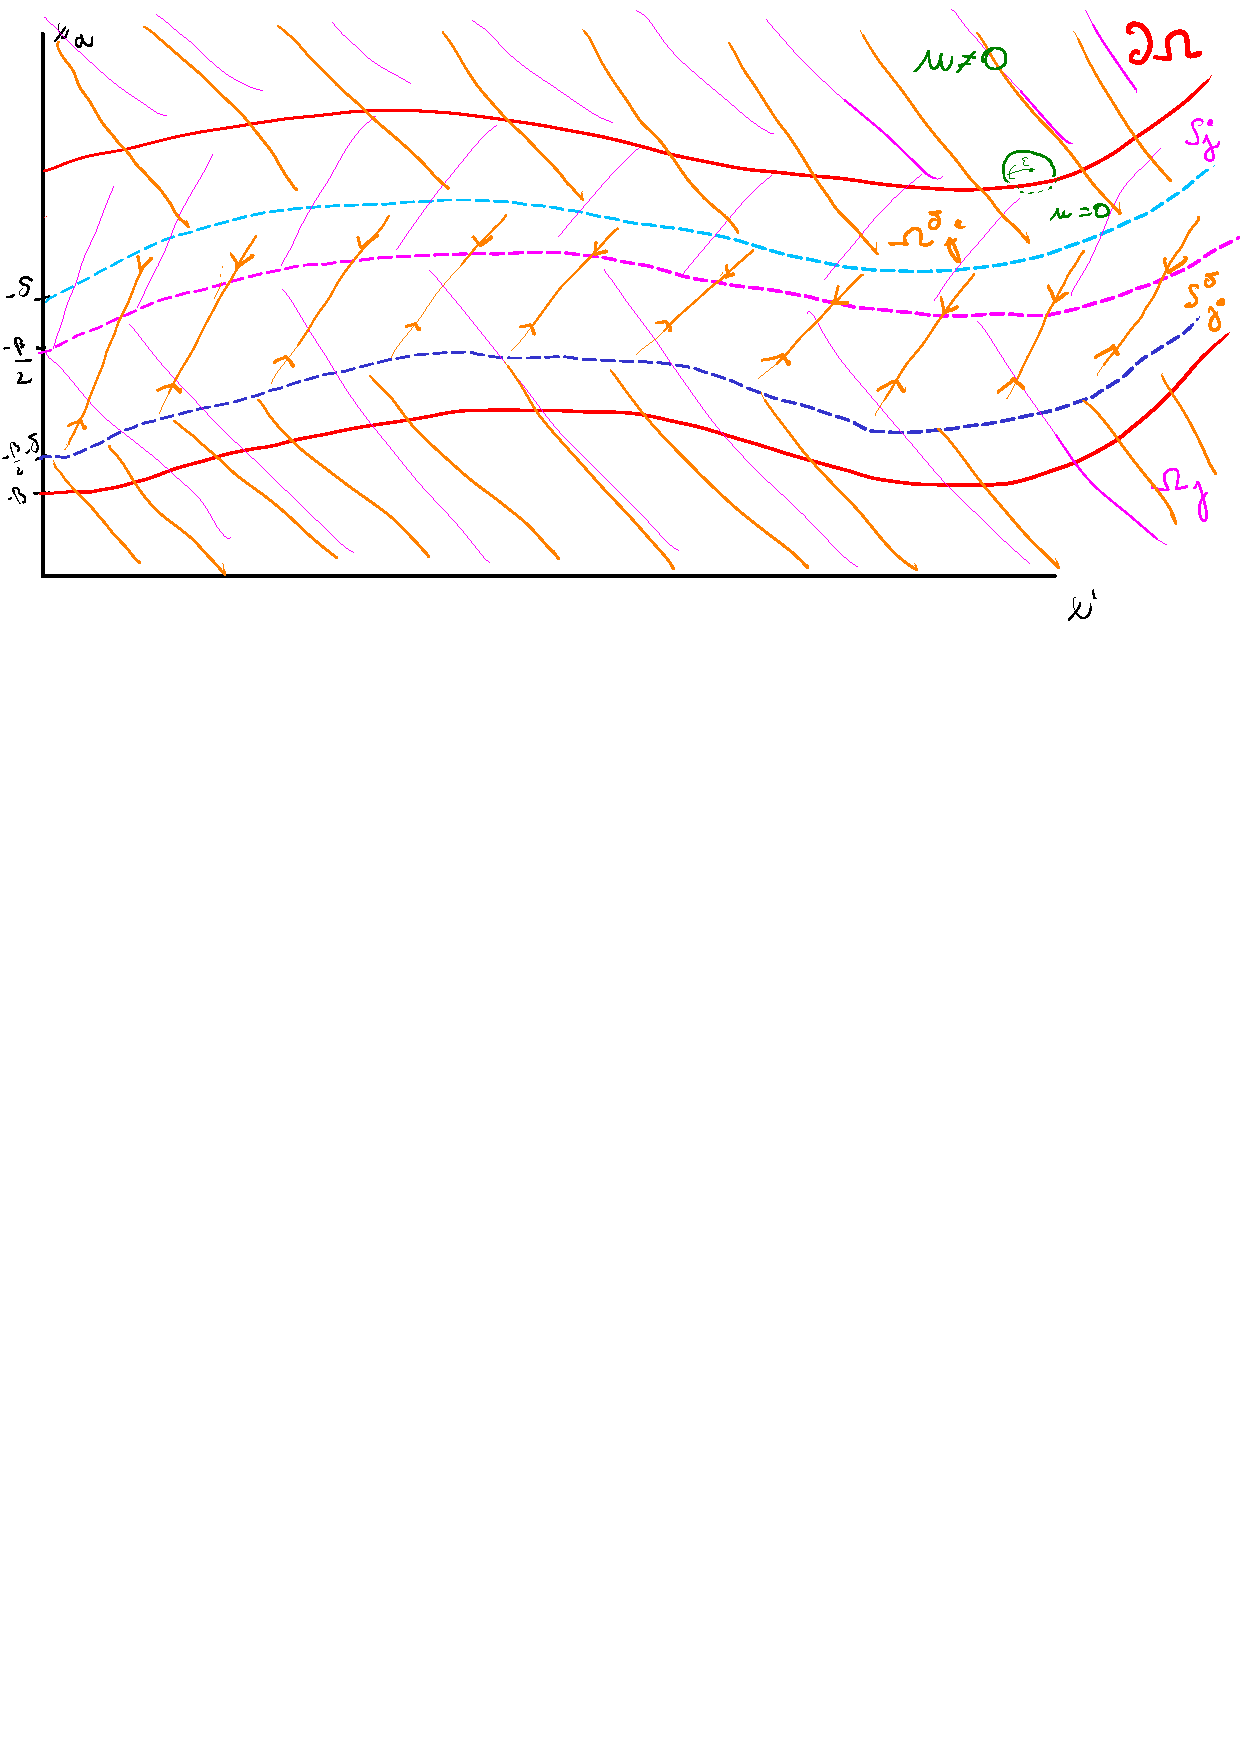
\includegraphics[width=\linewidth]{figures/mollification.pdf}
	  \caption{A cumbersome sketch of $\Omega_j, S_j, \Omega_j^{\delta}, S_j^{\delta}$}
	  \label{fig:mollification}
  \end{center}
\end{figure}

	\textit{Case $j \in \{1,\dots,m\} $}.
	We have a problem now: $\qty{U_j}_{j=1}^m$ covers $\partial \Omega,$ which is a \textit{closed} set and we cannot simply use local approximation theorem. One could imagine if we were to mollify in the neighbourhood of $\partial \Omega,$ the kernel would pick up values from outside of $\Omega,$ where $u=0$ and the mollification would not be a good approximation. Instead, we approximate $u_j$ on a larger \textit{open} domain containing $\overline{\Omega}$ and then show this is also a good aproximation of $u_j$ on $\Omega \subset \overline{\Omega}.$

	Set $w_j = u \varphi_j,$ and denote
	\begin{align*}
		S_j &=\tensorq{A}_j\qty(\qty{(x',x_d) | a_j(x') - \frac{\beta}{2}  < x_d < a_j(x') , x' \in \text{U}(0,\alpha)}), \\
	\Omega_j &= \R^{d} / \overline{S_j},
	\end{align*}
	\textit{i.e.},
	\[
		"\Omega_j = \Omega \cup \tensorq{A}_j\qty(\qty{(x',x_d)| x_d \leq a_j(x')- \frac{\beta}{2}}),"
	\]
	(although this is a bit inaccurate). Realize that since $u = 0$ outside of $\Omega,$ also $u_j$ is zero there and in particular it is zero on that "lower strip". Clearly then $u_j \in \WkpSet{\Omega_j}.$ Now pick $\delta \in \qty(0,\frac{\beta}{2}),$ where $\beta$ is from the definition of $\Ckl{0}{0}$ and set
	\begin{align*}
	  		S_{j}^{\delta} &= \tensorq{A}_j\qty(\qty{(x',x_d) | a_j(x') - \frac{\beta}{2} - \delta < x_d < a_j(x') -\delta, x' \in \text{U}(0,\alpha)}), \\
		\Omega_j^{\delta} &= \R^{d} / \overline{S_{j}^{\delta}}, 
	\end{align*}
	\textit{i.e.},
	\[
		"\Omega_j^\delta = \Omega \cup \tensorq{A}_j\qty(\qty{(x',x_d)| a_j(x')-\delta < x_d < a_j (x')}) \cup \tensorq{A}_j \qty(\qty{(x',x_d)| x_d < a_j(x') - \frac{\beta}{2} - \delta})."
	\]
The trick is to shift the (support of) function $u_j$ "into" $\Omega_{j}^\delta$

	\[
		\tau_{\delta}u_j\qty(\tensorq{A}_j\qty(x', a_j(x'))) = u_j\qty(\tensorq{A}_j\qty(x', a_j(x') + \delta)), x' \in \text{U}(0,\alpha) \subset \R^{d-1}.
	\]
	Realize that in fact
	\[
		\supp\qty(\tau_{\delta}u_j) = \supp\qty(u_j) - \delta,
	\]
	from which it follows $\tau_{\delta}u_j \in \WkpSet{\Omega_j^{\delta}};$ we have only shifted the function $u_j$, but since we have also shifted $S_j$, qualitatively there is no difference. Since $ \Omega \subset \Omega_j^\delta \subset \Omega_j^{\delta} \cap \Omega_j, \Omega \subset \Omega_j \subset \Omega_j^{\delta} \cap \Omega_j,$ and the fact $\tau_{\delta}$ is an isometry between Sobolev spaces, we also have $u_j, \tau_{\delta}u_j \in \WkpSet{\Omega_{j} \cap \Omega_j^{\delta}}.$ Moreover, from the properties of the shift operator it follows $\exists \delta >0$ \textit{s.t.}
	\[
		\norm{u_j - \tau_{\delta}u_j}_{\WkpSet{\Omega}}\leq \norm{u_j - \tau_{\delta}u_j}_{\WkpSet{\Omega_j \cap \Omega_j^{\delta}}} < \frac{\varepsilon}{2\qty(m+1)}.
	\]

	We are on a good track. Since we know $\tau_{\delta}u_j$ is already close to $u_j,$ we are done once we approximate $\tau_{\delta}u_j$ by a function from $\CinfSet{\overline{\Omega}}.$ Notice that if we show $\overline{\Omega} \subset \Omega_j^{\delta},$ then clearly $\CinfSet{\Omega_j^{\delta}} \subset \CinfSet{\overline{\Omega}}.$

\textit{Show $\Omega \subset \subset \Omega_j^{\delta}$:}
We already know $\Omega \subset \Omega_j^{\delta},$ so it suffices to show $\partial \Omega \subset \Omega_j^{\delta}.$ Our parametrization of the boundary yields
\[
	\partial \Omega = \bigcup_{k=1}^m \tensorq{A}_k\qty(\qty{(x',x_d)| x_d = a_k(x'), x' \in \text{U}(0,\alpha)}),
\]
and the set $\Omega_j^{\delta}$ is given as $\Omega_{j}^{\delta} = \R^{d} / \overline{S_j},$ where
\[
	S_j = \tensorq{A}_j\qty(\qty{(x',x_d)| a_j(x') - \frac{\beta}{2} - \delta < x_d < a_j(x') - \delta, x' \in \text{U}(0,\alpha)}).
\]
Realize it suffices to show $\partial \Omega \not \subset \overline{S_j}$, as then it wont be excluded from $\R^{d}$ and thus will end up in $\Omega_j^\delta.$ \textit{Thanks to continuity of $a_j$}, we may write
\[
	\overline{S_j} = \tensorq{A}_j\qty(\qty{(x',x_d)| a_j(x') - \frac{\beta}{2} - \delta \leq x_d \leq a_j(x') - \delta, x' \in \text{U}(0,\alpha)}),
\]
\textit{i.e.}, the $"<"$ have changed to $"\leq"$. Since we are doing everything locally, it is enough to show
\[
	\tensorq{A}_j\qty(\qty{(x',x_d)|x_d = a_j(x'), x' \in \text{U}(0,\alpha)}`) \not \subset \tensorq{A}_j\qty(\qty{(x',x_d)| a_j(x') - \frac{\beta}{2} - \delta \leq x_d \leq a_j(x') - \delta, x' \in \text{U}(0,\alpha)}),
\]
which is equivalent to
\[
	\qty((a_j \leq a_j - \delta) \wedge (a_j < a_j - \frac{\beta}{2} - \delta)) \vee \qty((a_j > a_j - \delta) \wedge (a_j \geq a_j - \frac{\beta}{2} - \delta)).
\]
Our choice has been $\delta \in \qty(0, \frac{\beta}{2}),$ and $\beta > 0$ from the definition of $\Omega \in \Ckl{0}{0},$ so the second statement is clearly true $\forall j \in {1, \dots, m}$. Consequently $\partial \Omega \not \subset \overline{S}_j$ which leads to $\partial \Omega \subset \Omega_j^{\delta},$ and since also $\Omega \subset \Omega_j^{\delta},$ we have $\overline{\Omega} \subset \Omega_j^{\delta}.$

\textit{Approximation of $\tau_{\delta}u_j$.}
Since $\Omega_{j}^\delta$ is open there $\exists w_j \in \CinfSet{\Omega_j^{\delta}}$ such that
\[
	\norm{\tau_{\delta}u_j - w_j}_{\WkpSet{\Omega}} \leq \norm{\tau_{\delta}u_j - w_j}_{\WkpSet{\Omega_{j}^\delta}} < \frac{\varepsilon}{4(m+1)}.
\]
What is more, since $\overline{\Omega} \subset \Omega_j^{\delta},$ we see $w_j \in \CinfSet{\overline{\Omega}}$ in fact. What is even more, we see $\supp w_j \subset \supp u_j - \delta$ so $\supp \tau_{-\delta} w_j \subset \supp u_j \subset \subset \Omega,$ and since $w_j$ is defined on the whole $\R^{d},$ also $v_j \coloneq \tau_{-\delta}w_j$ is defined on the whole $\R^{d}.$ Alltogether, $v_j = \tau_{-\delta}w_j \in \DSet{\R^{d}},$ and from the properties of the shift operator, there $\exists \delta >0$ \textit{s.t.}
\[
	\norm{v_j - w_j}_{\WkpSet{\Omega}} < \frac{\varepsilon}{4\qty(m+1)}.
\]


\textit{Approximation of $u$.}

Finally, let us set
\[
	v = \sum_{j=0}^m v_j.
\]
Then $v \in \DSet{\R^{d}}$ and it holds
\begin{align*}
	\norm{u-v}_{\WkpSet{\Omega}} &= \norm{\sum_{j=0}^m u_j- \sum_{j=0}^m v_j}_{\WkpSet{\Omega}} = \norm{\sum_{j=0}^m u_j - v_j}_{\WkpSet{\Omega}} \leq \sum_{j=0}^m \norm{u_j - v_j}_{\WkpSet{\Omega}} \leq \\
	& \leq \frac{\varepsilon}{m+1} + \sum_{j=1}^m \norm{v_j-u_j}_{\WkpSet{\Omega}} \leq \frac{\varepsilon}{m+1} + \sum_{j=1}^m \norm{v_j - w_j}_{\WkpSet{\Omega}} + \sum_{j=1}^m \norm{w_j - \tau_{\delta}u_j}_{\WkpSet{\Omega}} + \sum_{j=1}^m \norm{\tau_{\delta}u_j - u_j}_{\WkpSet{\Omega}}\\
	&< \frac{\varepsilon}{m+1} +  2\sum_{j=1}^m \frac{\varepsilon}{4\qty(m+1)} + \sum_{j=1}^m \frac{\varepsilon}{2\qty(m+1)} = \varepsilon
\end{align*}
Finally,
\[
	\DSet{\R^{d}} \subset \, \text{C} \,^{\infty}_{\overline{\Omega}}\qty(\R^{d}) \subset \CinfSet{\overline{\Omega}}.
\]

\textit{This proof may still have some flaws, but the author has decided to move on.}
\end{proof}	

\begin{remark}[What is $\, \text{C} \,^{\infty}_{\overline{\Omega}}\qty(\R^{d})$]
	Recall
	\[
		C^\infty_{\overline{\Omega}}(\R^d) = \Big\{u|_{\overline{\Omega}}, u \in C^{\infty}(\R^d) \Big\}.
	\]
\end{remark}



\subsection{Extension of Sobolev functions}
\label{sec:extension}

\textit{Problem of extension}: For $u \in \WkpSet{\Omega}$, does there exist
\[
	\overline{u} \in \WkpSet{\R^d}, \, \text{\textit{s.t.}} \,\overline{u}|_{\Omega}=u, \norm{\overline{u}}_{\WkpSet{\R^d}} \leq C(\Omega) \norm{u}_{\WkpSet{\Omega}}
\]

?

The answer is \textbf{yes}, if $\Omega$ is nice enough. Notice however this is not as simple as in the case of Lebesgue spaces, where we could just extend the function by zero trivailly. We are dealing with derivatives, that are somehow regular, and if we extend a nonzero function by zero, it might mess up the regularity of the derivatives.

We will be using $\, \text{C} \,^1$ diffeomorphisms heavily, so we investigate some of their properties first.

\begin{lemma}[Properties of $C^1$ diffeomorphisms]
	Let $U,V \subset \R^d$ be open, $\Phi: U \to V$ be a $C^1$ diffeomorphism and let $\tilde{U} \subset \R^{d}\, \text{\textit{s.t.}} \, \tilde{U} \subset \subset U$. Then
	\begin{enumerate}
		\item $\Phi(\tilde{U}) \subset \subset V,$
		\item if moreover $\tilde{U}$ is compact, then \footnote{For $\tilde{U}$ compact: $\tilde{U} \subset \subset V \Leftrightarrow \tilde{U} \subset V$.} 
			\[
				\exists C>0: \forall u \in C^1\qty(V): \norm{u \circ \Phi}_{\WkpSet[1][p]{\tilde{U}}} \leq C \norm{u}_{\WkpSet[1][p]{\Phi(\tilde{U})}}.
			\]
	\end{enumerate}
\end{lemma}

\begin{proof}

	\textit{Ad 1.}: No proof has been given.


	\textit{Ad 2.}: Just a change of variables formula:
	\[
		\norm{u \circ \Phi}_{\LpSet{\tilde{U}}}^p = \int_{\tilde{U}}|u \circ \Phi|^p\dd{x} = \int_{\Phi\qty(\tilde{U})}|u|^p | \det \grad \Phi|^{-1}\dd{x}.
	\]
	Since $\Phi$ is one-to-one, we know $|\det \grad \Phi| >0$ on $U$, and since $\Phi \in \CkSet{1}{U}$ and $\tilde{U} \subset U \Rightarrow \Phi \in \CkSet{1}{\tilde{U}} \Rightarrow \det \grad \Phi \in \CkSet{0}{\tilde{U}},$ and since $\tilde{U}$ is compact, $|\det \grad \Phi| \geq C_1 > 0 \Leftrightarrow |\det \grad \Phi|^{-1}\leq \frac{1}{C_1}.$ In total	
	\[
		\norm{u \circ \Phi}_{\LpSet{\tilde{U}}}^p \leq \frac{1}{C_1} \int_{\Phi(\tilde{U})}|u|^p\dd{x} = C\norm{u}_{\LpSet{\Phi(\tilde{U})}}^p.
	\]
	As for the derivative, we have $\forall i \in \qty{1,\dots,d}:$
	\begin{align*}
		\int_{\tilde{U}}|\partial_{i}(u \circ \Phi)|^p\dd{x} &\leq \int_{\tilde{U}}|\grad (u \circ \Phi)|^p\dd{x} = \int_{\tilde{U}}| \grad \Phi \Big(\qty(\grad u)\circ \Phi\Big)|^p\dd{x}\leq \\
									 &\leq \norm{\grad \Phi} \int_{\tilde{U}}|(\grad u) \circ \Phi|^p\dd{x} = \norm{\grad \Phi} \int_{\Phi\qty(\tilde{U})}|\grad u|^p |\det \grad \Phi|^{-1}\dd{x} \leq C\norm{\grad \Phi} \int_{\Phi\qty(\tilde{U})}|\grad u|^p\dd{x} \leq \\
										 &\leq C \norm{\grad u}_{\LpSet[p]{\Phi\qty(\tilde{U})}}^p,
	\end{align*}
	where $\norm{\grad \Phi}$ is \textit{e.g.} the operator norm of the matrix $\grad \Phi.$
\end{proof}


\begin{lemma}[Flat extension]
	Let $\alpha, \beta >0, K \subset \subset U(0,\alpha) \times [0,\beta)$ be compact. Then there $\exists C >0 $, a linear operator
	\[
		E:\CkSet{1}{(\text{B}(0,\alpha) \cross [0,\beta])} \to \CkSet{1}{(\text{B}(0,\alpha) \cross [-\beta, \beta])}, 
	\]
	and the set $\tilde{K} \subset \subset \text{U}(0,\alpha) \times [-\beta, \beta)$ such that $\forall u \in \CkSet{1}{\text{B}(0,\alpha) \times [0,\beta]})$ it holds
	\begin{enumerate}
		\item $Eu = u$ on $\text{B}(0,\alpha) \times [0,\beta]$,
		\item $\norm{Eu}_{\WkpSet[1][p]{\text{U}(0,\alpha) \times (-\beta,\beta)}} \leq \norm{u}_{\WkpSet[1][p]{\text{U}(0,\alpha) \times (0, \beta)}} $. Actually,
			\[
				\norm{E}_{\mathcal{L}\qty(\WkpSet[1][p]{\text{U}(0,\alpha)\times (0,\beta)},\WkpSet[1][p]{\text{U}(0,\alpha)\times(-\beta,\beta)})} = 2^{\frac{1}{p}}
			\]
		\item if $\supp u \subset K \, \text{then} \,\supp Eu \subset \tilde{K}$
	\end{enumerate}
\end{lemma}

\begin{proof}
	(The set $\text{U}(0,\alpha) \times [0,\beta)$ is a cylinder of radius $\alpha$ and height $\beta$)

	The proof is constructive: for the assumed $u$ we write ($x = (x',x_d),$ where $x' \in \text{B}(0,\alpha) \subset \R^{d-1}, x_d \in [0,\beta] \subset \R$)

	\begin{equation*}
		Eu(x',x_d) = 
		\begin{cases}
			u(x',x_d),& x_d \geq 0 \\
			-3u(x',-x_d) + 4u(x' ,-\frac{x_d}{2}) ,& x_d < 0.\\
		\end{cases}
	\end{equation*}
	Does $Eu$ lie in $\CkSet{1}{\text{B}(0,\alpha)\times [-\beta, \beta]}$? Since $u \in \CkSet{1}{\text{B}(0,\alpha)\times [0,\beta]}$, it us continuous in the "lower cylinder", check only the transition through the origin plane: take some $a=(x',0) \in \text{B}(0,\alpha)\times \qty{0}$. Then

	\begin{equation*}
		\lim_{x \to a} Eu(x) = 
		\begin{cases}
			u(a), & x_d \geq 0 \\
			-3u(a)+ 4u(a) = u(a), & x_d<0, \\
		\end{cases}
	\end{equation*}
	so $Eu$ is continuous. The derivatives 

	\begin{equation*}
		\lim_{x\to a}\partial_{d} Eu(x',x_d) = 
		\begin{cases}
			\partial_{d}u(x', 0) ,& x_d \geq 0 \\
			\eval{\qty(-3 \partial_{d} u (x',-x_d)(-1) + 4 \partial_{d}u(x',-\frac{x_d}{2}) (-\frac{1}{2}))}_{x_d = 0} = \partial_{d} u(x', 0),& x_d<0,\\
		\end{cases}
	\end{equation*}
	and also for any $i \in \qty{1, \dots, d-1}$ 
	\begin{equation*}
	  \lim_{x\to a}\partial_{i} Eu(x_1, \dots, x_d) = 
	  \begin{cases}
		  = \partial_{i} u (x_1, \dots, 0) , & x_d \geq 0 \\
		  = -3 \partial_{i} u(x_1, \dots, 0) + 4 \partial_{i} u(x_1, \dots, 0) = \partial_{i} u(x_1, \dots, 0)
	  \end{cases}
	\end{equation*}
	
	so the the derivative is also continuous. Thus, we have
	\[
		Eu  \in C^1 \subset \WkpSet[1][p]{U(0,\alpha) \cross (-\beta,\beta)}.
	\]
	The first property is clear from the definition of $Eu$, the estimates of the norm: (all derivatives can in fact be assumed classical)
	\begin{align*}
		\norm{Eu}_{\WkpSet[1][p]{\text{U}(0,\alpha) \times (-\beta,\beta)}}^p &= \norm{Eu}_{\LpSet{\text{U}(0,\alpha)\times (-\beta,\beta)}}^p + \sum_{|\alpha| = 1}\norm{D^{\alpha}Eu}_{\LpSet{\text{U}(0,\alpha)\times (-\beta, \beta)}}^p = \\
		&= \norm{Eu}_{\LpSet{\text{U}(0,\alpha) \times (0,\beta)}}^p +\norm{Eu}_{\LpSet{\text{U}(0,\alpha) \times (-\beta,0)}}^p \\ +
		& + \sum_{|\alpha| = 1}\norm{D^{\alpha}Eu}_{\LpSet{\text{U}(0,\alpha)\times (0, \beta)}}^p + \sum_{|\alpha| = 1}\norm{D^{\alpha}Eu}_{\LpSet{\text{U}(0,\alpha)\times (-\beta, 0)}}^p = \\
		& = \norm{u}_{\LpSet{\text{U}(0,\alpha)\times (0,\beta)}}^p + \norm{4u - 3u}_{\LpSet{\text{U}(0,\alpha)\times (-\beta, 0)}}^p + \\
		& + \sum_{|\alpha| = 1}\norm{D^{\alpha}u}_{\LpSet{\text{U}(0,\alpha)\times (0,\beta)}}^p + \sum_{|\alpha| =1}\norm{D^{\alpha}\qty(4u - 3u)}_{\LpSet{\text{U}(0,\alpha)\times (-\beta,0)}}^p \\
		&= 2 \norm{u}_{\LpSet{\text{U}(0,\alpha)\times (0,\beta)}}^p + 2 \sum_{|\alpha| =1}\norm{D^{\alpha}u}_{\LpSet{\text{U}(0,\alpha)\times (0,\beta)}}^p = 2 \norm{u}_{\WkpSet{\text{U}(0,\alpha)\times (0,\beta)}}^p
	\end{align*}
	and so
	\[
		\norm{Eu}_{\WkpSet[1][p]{\text{U}(0,\alpha)\times (-\beta,\beta)}} = 2^{\frac{1}{p}} \norm{u}_{\WkpSet[1][p]{\text{U}(0,\alpha)\times (0,\beta)}}.
	\]
	Where we have used the obvious fact
	\[
		\int_{\text{U}(0,\alpha)\times (0,\beta)}|f|^p\dd{x} = \int_{\text{U}(0,\alpha)\times (-\beta,0)}|f|^p\dd{x},
	\]

	We will assume (although this is \textit{with} a loss of generality), that
	\[
		Eu\qty(x', x_d) = 0 \Leftrightarrow (u(x', x_d) = 0 \vee 3u(x',-x_d) = 0 \vee 4u(x', - \frac{x_d}{2})= 0),
	\]
	\textit{i.e.}, that support lies in
	\begin{align*}
		\supp Eu &\subset\qty{(x',x_d) \in \text{U}(0,\alpha) \times [0, \beta] | u(x', x_d) = 0} \cup \qty{(x',x_d) \in \text{U}(0,\alpha) \times [-\beta,0]| u(x', - x_d) \neq 0}\cup \\
			 &\cup \qty{(x',x_d) \in \text{U}(0,\alpha) \times [-\beta,0]| u(x', - \frac{x_d}{2}) \neq 0}.
	\end{align*}
	Denote $\Phi_1, \Phi_2: \text{U}(0,\alpha) \times (0,\beta) \to \text{U}(0,\alpha) \times (-\beta,\beta)$ to be the mappings
	\begin{align*}
		\Phi_1 (x',x_d) &= (x', -x_d),\\
		\Phi_2 (x',x_d) &= (x', - \frac{x_d}{2}),
	\end{align*}
	then clearly $\Phi_1, \Phi_2$ are $\, \text{C} \,^1$ diffeomorphisms and
	\[
		u(x',-x_d) = \qty(u \circ \Phi_1)(x',x_d), u\qty(x', - \frac{x_d}{2}) = \qty(u \circ \Phi_2)\qty(x',x_d),
	\]
	\textit{i.e.},
	\[
		u\qty(x',x_d) = \qty(u \circ \Phi_1^{-1})\qty(x', -x_d) = \qty(u \circ \Phi_2^{-1})\qty(x',-\frac{x_d}{2}),
	\]
	and so
	\[
		\supp Eu \subset \supp u \cup \Phi_1^{-1}\qty(\supp u) \cup \Phi_2^{-1}\qty(\supp u) \subset K \cup \Phi_1^{-1}\qty(K) \cup \Phi_2^{-1}\qty(K),
	\]
	as $\supp u \subset \subset K.$ Let us define
	\[
		\tilde{K} \coloneq K \cup \Phi_1^{-1}\qty(K) \cup \Phi_2^{-1}\qty(K),
	\]
	Then we see
	\[
		\supp Eu \subset K \cup \Phi_1^{-1}\qty(K) \cup \Phi_2^{-1}\qty(K) = \tilde{K},
	\]
	And, finally, we have $K \subset \subset \text{U}(0,\alpha) \times [0,\beta) \Rightarrow K \subset \subset \text{U}(0,\alpha) \times (-\beta,\beta) \Rightarrow \Phi_1^{-1}\qty(K), \Phi_2^{-1}\qty(K)\subset \subset \text{U}(0,\alpha)\times (0,\beta),$ which really implies
	\[
		\tilde{K} \subset \subset \text{U}(0,\alpha) \times [-\beta, \beta).
	\]
\end{proof}

Let us prove the main result.

\begin{theorem}[Extension of Sobolev functions]
	Let $\Omega \in C^{k-1,1}, k \in \N, p \in [1,\infty], V \subset \R^d$ open such that $\Omega \subset \subset V.$ Then there is $E: \WkpSet{\Omega} \to \WkpSet{\R^d}$ bounded linear operator such that
	\begin{enumerate}
		\item $ \forall u \in \WkpSet{\Omega}: Eu=u \, \text{\textit{a.e.}} \,\, \text{in} \, \Omega$,
		\item $ \forall u \in \WkpSet{\Omega}: \supp Eu \subset V \supset \supset \Omega$,
		\item $\norm{E}_{\mathcal{L}\qty(\WkpSet{\Omega},\WkpSet{\R^{d}})} \leq C, C=C(p,\Omega,V).$
	\end{enumerate}
\end{theorem}

\begin{proof}
	\textbf{Will only be presented for $k=1, \Omega \in C^1, p < \infty$.} The strategy is:
	\begin{enumerate}
		\item covering of $\overline{\Omega}$ \& partition of unity
		\item obtain a diffeomorphism from the fact $\Omega \in \Ckl{1}{0},$
		\item suitable composition \& cut off,
		\item flat extension,
		\item show existence of $E: \, \text{C} \,^{\infty}_{\overline{\Omega}}\qty(\R^{d})\to \WkpSet{\R^{d}}$ with the desired properties,
		\item extend via density
	\end{enumerate}

	\textit{Covering of $\Omega$:}
	In the following,  $U_j,a_j, \tensorq{A}_j, \alpha, \beta$ are as in the definition of a $\Ckl{1}{0}$ domain. Set $U_0 = \Omega$ and realize
	\[
		\overline{\Omega} \subset \bigcup_{j=0}^m U_j,
	\]
	\textit{i.e.}, $\qty{U_j}_{j=0}^m$ is an open covering of $\overline{\Omega}$. Denote $\{\varphi_j \}_{j=0}^m$ as the partition of unity subordinate to $\{U_j\}_{j=0}^m.$


	\textit{Diffeomorphism \& flat extension}
	For $j \in \{1, \dots, m\}$ we define $\Phi_j : \text{U}(0,\alpha) \cross (-\beta,\beta) \to U_j$ by
	\[
		\Phi_j\qty(y',y_d) = \tensorq{A}_j (y', a_j(y') + y_d), y' \in \R^{d-1}, y_d \in \R.
	\]

	(A bit confusingly, we will however be "interpreting" $\Phi_j$ as $\Phi_j : \text{U}(0,\alpha) \times \qty(-\beta, \beta) \to \R^{d},$ with it being extended by zero on $\R^{d}/ \overline{U_j},$ as we need $\Phi_j^{-1}$ to be defined on the whole $\R^{d}.$)

	As $\Omega \in \Ckl{1}{0},$ we know $a_j \in \CkSet{1}{\text{B}(0,\alpha)}\subset \CkSet{1}{\text{U}(0,\alpha)},$ and so $\phi_j$ is a $\text{C}^1$ diffemorphism. Let us denote by $\tilde{E}: \CkSet{1}{\text{B}(0,\alpha)\times [-\beta, \beta]} \to \CkSet{1}{\text{B}(0,\alpha)\times [-2 \beta, \beta]}$ the extension operator from the Flat extension lemma. Then we for any $u \in C^{\infty}_{\overline{\Omega}}\qty(\R^d): u = \sum_{j=1}^m \varphi_j u$ define
	\[
		Eu=\varphi_0 u + \sum_{j=1}^m \qty(\eta \tilde{E}\qty((\varphi_j u) \circ \Phi_j)) \circ \inverse{\Phi_j},
	\]
	where $\eta \in \CinfSet{\text{U}(0,\alpha)\times \R}$ is a cut-off function
	\begin{equation*}
		\eta\qty(y',y_d)  
		\begin{cases}
			=1 \, \text{on} \, &y_d \geq 0,\\
			= 0 \, \text{on} \,& y_d \leq -h, \\
			\in (0,1) \, &\text{else} \,.
		\end{cases},
	\end{equation*}
for some parameter $h>0$ which will be defined later.
With this definition, $\forall x \in \Omega$ it holds
\begin{align*}
	\qty(Eu)(x) &= \qty(\varphi_0 u)(x) + \sum_{j=1}^{m}\qty(\eta \tilde{E}\qty(u \varphi_j \circ \Phi_j))\underbrace{\qty(\Phi_j^{-1}(x))}_{\in \text{U}(0,\alpha)\times \qty(-\beta, \beta)} =\\
	&= \qty(\varphi_0 u)(x) + \sum_{j=1}^m \qty(u \varphi_j \circ \Phi_j)\qty(\Phi_j^{-1}(x)) = \qty(\varphi_0 u)(x) + \sum_{j=1}^m \qty(u \varphi_j)(x) = \sum_{j=0}^m \qty(u \varphi_j)(x) = u(x) \sum_{j=0}^m \varphi_j(x) = u(x),
\end{align*}
since $\eta(y) = 1, \tilde{E}\qty(\varphi_j u \circ \Phi_j) (y) = \qty(\varphi_j u \circ \Phi_j)(y)$ for $y \in \text{U}(0,\alpha) \times (-\beta, \beta), $ according to our definition of $\eta$ and the properties of the extension $\tilde{E}.$

The motivation behind the cutoff is the following: we know $\supp \varphi_j \subset U_j,$ so since $\Phi_j: \text{U}(0,\alpha)\times(-\beta,\beta) \to U_j, $ we have $\supp u \varphi_j \circ \Phi_j \subset \text{U}(0,\alpha)\times (-\beta, \beta)$ and from the properties of the flat extension operator we also have $\supp \tilde{E}\qty(u \varphi_j \circ \Phi_j) \subset \text{U}(0,\alpha)\times (-2 \beta, \beta)$. Since moreover $\supp \eta = \text{U}(0,\alpha) \times (-2h, \infty),$ in total
\[
 \supp \eta \tilde{E}\qty(u \varphi_j \circ \Phi_j) = \supp \eta \cap \supp \tilde{E}\qty(u \varphi_j \circ \Phi_j) = \text{U}(0,\alpha) \times (-2h, \infty) \cap (-\beta, \beta),
\]
and also \footnote{Generally, $\supp v \circ \Psi^{-1} = \overline{\qty{x \in \R^{d}| u\qty(\Psi^{-1}(x)) \neq 0}} = \overline{\qty{x \in \R^{d}| \Psi^{-1}(x) \in \supp u}} = \overline{\qty{x \in \R^{d}| x \in \Psi\qty(\supp u)}} = \Psi\qty(\supp u).$}
\[
	\supp Eu \subset \Phi_j\qty(\supp \eta \tilde{E}\qty(u \varphi_j \circ \Phi_j)).
\]
We need to prove $\supp Eu \subset V,$ where $V$ is some neighbourhood of $\Omega$. If it holds
\[
	\supp \eta \tilde{E}\qty(u \varphi_j \circ \Phi_j) \subset \text{U}(0,\alpha) \times (-\beta,\beta),
\]
the desired property holds, as then
\[
	\supp Eu \subset \Phi_j \qty( \supp \eta \tilde{E}\qty(u \varphi_j \circ \Phi_j)) \subset \Phi_j\qty(\text{U}(0,\alpha)\times (-\beta, \beta)) \subset U_j \subset \overline{\Omega} \subset V.
\]
In total,  
\[
	\supp \eta \tilde{E}\qty(u \varphi_j \circ \Phi_j) = \text{U}(0,\alpha) \times (-2h, \infty) \cap (-\beta, \beta) \subset \text{U}(0,\alpha) \times (-\beta,\beta).
\]
So if $h$ is such that $-2h > -\beta \Leftrightarrow h < \frac{\beta}{2}$, we can guarantee $\supp Eu \subset V$ and that is what we want.

Finally, $E$ is clearly linear, its norm: (we are using the lemma about flat extension and the properties of $\, \text{C} \,^1$ diffeomorphisms together with the facts $ \eta \leq \, \text{on} \, \text{U}(0,\alpha) \times (-\beta, \beta),$ $\Phi_j\qty(\text{U}(0,\alpha)\times (0,\beta)) \subset U_{j},$$ \Phi_j^{-1}\qty(\R^{d}) \subset \footnote{We can somehow extend $\Phi_j^{-1}$ by zero from $U_j \subset \Omega \subset \R^{d}$ to be defined on the whole $\R^{d}$ (i guess)}, \text{U}(0,\alpha)\times \qty(-\beta,\beta)$, \footnote{...even though the assumptions to use those are not totally valid... but doc. Kaplicky is okay with that})

\begin{align*}
\norm{Eu}_{\WkpSet[1][p]{\R^{d}}} &= \norm{\qty(\eta \tilde{E}\qty(\varphi u_j \circ \Phi_j))\circ \Phi_j^{-1}}_{\WkpSet[1][p]{\R^{d}}} \leq C\norm{\eta \tilde{E} \qty(\varphi u_j \circ \Phi_j)}_{\WkpSet[1][p]{\text{U}(0,\alpha)\times (-\beta,\beta)}} = \\
				  &= C \norm{\tilde{E}\qty(u \varphi_j \circ \Phi_j)}_{\WkpSet[1][p]{\text{U}(0,\alpha)\times (-\beta, \beta)}} \leq C \norm{u \varphi_j \circ \Phi_j}_{\WkpSet[1][p]{\text{U}(0,\alpha)\times (0,\beta)}} \leq \\
				  &\leq C \norm{u \varphi_j}_{\WkpSet[1][p]{U_j \cap \Omega}} \leq C \norm{u}_{\WkpSet[1][p]{\Omega}},
\end{align*}
from which it clearly follows $\norm{E}_{\mathcal{L}\qty(\WkpSet[1][p]{\Omega}, \WkpSet[1][p]{\R^d})} \leq C.$

	So all the properties hold for $u \in C^{\infty}_{\overline{\Omega}}\qty(\R^d)$, let us show them also for $u \in \WkpSet[1][p]{\Omega}$.
	Pick an arbitrary $u \in \WkpSet[1][p]{\Omega}, \, \text{find} \, \{u_k\} \subset C^{\infty}_{\overline{\Omega}}\qty(\R^d): u_k \to u \, \text{in} \, \WkpSet[1][p]{\Omega}.$ Since $E$ is continous, we know $\lim_{k\to \infty}E u_k$ exists. Let us set
	\[
		E u \coloneq \lim_{k\to \infty}E u_k,
	\]
	where $Eu_k$ is defined above for $u_k \in \, \text{C} \,^{\infty}_{\overline{\Omega}}\qty(\R^{d}).$

	Ad 3): Clearly $E \qty(\alpha u) = \lim_{k \to \infty}E \qty(\alpha u_k) = \alpha E u, E \qty(u + v) = \lim_{k\to \infty}E\qty(u_k + v_k) = \lim_{k \to \infty}Eu_k + Ev_k = Eu + Ev,$ since $E$ on the continous functions is linear. Also


	\[
		\norm{Eu}_{\WkpSet[1][p]{\R^{d}}} = \norm{\lim_{k\to \infty}E u_k}_{\WkpSet[1][p]{\R^{d}}} = \lim_{k\to \infty} \norm{E u_k}_{\WkpSet[1][p]{\R^{d}}} \leq \norm{E} \lim_{k\to \infty}\norm{u_k}_{\WkpSet[1][p]{\R^{d}}} = \norm{E} \norm{u}_{\WkpSet[1][p]{\R^{d}}},
	\]
	(we are using $\qty{E u_k}$ has a limit); we see our above definition truly yields a continuous linear operator.\\
	Ad 1): $\forall \, \text{\textit{a.a.}} \, x \in \Omega: Eu(x) = \lim_{k\to \infty}Eu_k(x) = \lim_{k \to \infty}u_k(x) = u(x),$\\
	Ad 2): $\supp Eu_k \subset \text{U}(\Omega,\varepsilon) \Rightarrow \supp Eu \subset \overline{\text{U}(\Omega,\varepsilon)} \subset V.$
	\[
		\supp Eu = \qty{x \in \R^{d}| \lim_{k\to \infty}Eu_k \neq 0}\subset \bigcap_{k=1}^{\infty}\underbrace{\supp Eu_k}_{\subset V} \subset V.
	\]
	We are done.

\end{proof}

\begin{remark}[$\Omega \in C^{0,1}$ suffices]
	The theorem is still valid if we assume only $\Omega \in \Ckl{0}{1}$ and $p \in (1,\infty), k \in \N,$ but the construction of the extension must be different. "It seems the result is not known for $\Omega \in \Ckl{0}{1}$ and $p = 1,$ or $p = \infty.$"
\end{remark}

\subsection{Embedding theorems}
\label{sec:embedding}

From the definition of $\WkpSet{\Omega}$ it immediately follows $\WkpSet{\Omega} \subset \LpSet{\Omega}.$ Can we obtain $\WkpSet{\Omega} \subset \LpSet[q]{\Omega}$ for some $q > p?$ The answer \textbf{yes}, if $\Omega$ is again nice enough (and there will also be some dependence on the dimension of $\R^{d}.$)

\subsubsection{Theorems for $p \leq d$}
\label{sec:embedding_p_leq_q}

\begin{example}
	Let $u \in \mathcal{D}\qty(\R^2)$. Then 

	\begin{equation*}
		u\qty(x_1,x_2) = \int_{-\infty}^{x_1} \partial_{1}u\qty(s,x_2)\dd{s} = \int_{-\infty}^{x_2} \partial_{2}u(x_1,s)\dd{s},
	\end{equation*}
	so 
	\begin{align*}
		\norm{u}_{\LpSet[2]{\R^{2}}}^{2} = \int_{\R^2}|u(x_1,x_2)|^{2}\dd{x_1} \dd{x_2} &= \int_{\R}\int_{\R}|u(x_1,x_2)|^{2}\dd{x_1}\dd{x_2}\leq \\
		&\leq \qty(\int_{\R}\int_{-\infty}^{x_1}|\partial_{1}u(s,x_2)|\dd{s}\dd{x_2}) \qty(\int_{\R}\int_{-\infty}^{x_2}|\partial_{2} u(x_1,s)|\dd{s}\dd{x_2}) \leq \\
		&\leq \qty(\int_{\R}\int_{\R}|\partial_{1}u(s,x_2)|\dd{s}\dd{x_2})\qty(\int_{\R}\int_{\R}|\partial_{2}u(x_1,s)|\dd{s}\dd{x_2}) \leq \\
		& \leq \qty(\int_{\R}\int_{\R}|\grad u(s,x_2)|\dd{s}\dd{x_2})\qty(\int_{\R}\int_{\R}|\grad u(x_1,s)|\dd{s}\dd{x_2}) = \\
		& = \qty(\int_{\R^2}|\grad u|\dd{x}) \qty(\int_{\R^{2}}|\grad u|\dd{x}) = \qty(\int_{\R^{2}}|\grad u|\dd{x})^{2} = \\
		& = \norm{\grad u}_{\LpSet[1]{\R^{2}}}^{2},
	\end{align*}
	so
	\[
		\norm{u}_{\LpSet[2]{\R^{2}}} \leq \norm{\grad u}_{\LpSet[1]{\R^{2}}}.
	\]
\end{example}

This can be generalized in two ways: 
\begin{itemize}
	\item $d > 2,$
	\item less smoothness.
\end{itemize}

\begin{lemma}[Gagliardo]
	Let $d\geq 2$. Let $\hat{u}_i:\R^{d-1} \to \R$ be nonnegative and measurable for $j \in \{1,\dots,d\}.$ We define
	\[
		\hat{x}_j = (x_1, \dots, x_{j-1}, x_{j+1}, \dots, x_d), \hat{\dd{x}_j} = \dd{x}_1 \dots \dd{x}_{j-1} \dd{x}_{j+1} \dots \dd{x}_d.
	\]
	Consider the functions $u_j:\R^d \to \R, u_j\qty(x)=\hat{u}_j(\hat{x}_j).$ Then
	\begin{equation}
		\int_{\R^d}\prod_{j=1}^d u_j\qty(x)\dd{x} \leq \prod_{j=1}^d \qty(\int_{\R^{d-1}}\qty(\hat{u}_j\qty(\hat{x}_j))^{d-1}\hat{\dd{x}_j})^{\frac{1}{d-1}}.
	\end{equation}
	(Both integrals can be infinity.)
\end{lemma}

\begin{proof}
	Induction by dimension:
	\textit{The case $d = 2$.}:
	\begin{align*}
		\int_{\R^{2}}u_1\qty(x_1,x_2)u_2\qty(x_1,x_2)\dd{x}_1 \dd{x}_2 &= \int_{\R^{2}}\hat{u}_1\qty(x_2) \hat{u}_2\qty(x_1)\dd{x}_1 \dd{x}_2 = \qty(\int_{\R}\hat{u}_1\qty(x_2)\dd{x}_2) \qty(\int_{\R}\hat{u}_2\qty(x_1)\dd{x}_1) = \\
		&=\qty(\int_{\R}\hat{u}_1\qty(\hat{x}_1)\hat{\dd{x}_1})\qty(\int_{\R}\hat{u}_2\qty(\hat{x}_2)\hat{\dd{x}_2}).
	\end{align*}
	(an equality in fact.) We have used Fubini once, which is permitted, as we have measurability + nonnegativity.

	\textit{The case $d \to d+1$}
	Before we procceed, recall the "generalized Holder", all functions are nonnegative

	\[
		\int_{\Omega}\prod_{j=1}^d f_j\dd{x} \leq \prod_{j=1}^d \qty(\int_{\Omega}f_j^{p_j}\dd{x})^{\frac{1}{p_j}},
	\]
	where $\sum_{j=1}^d \frac{1}{p_j}  = 1.$ See that if we take $p_j = d,$ then $\sum_{j=1}^d \frac{1}{d} = \frac{1}{d} \sum_{j=1}^d 1 =1,$ so
	\[
		\int_{\Omega}\prod_{j=1}^d f_j \dd{x} \leq \prod_{j=1}^d\qty(\int_{\Omega}f_j^d\dd{x})^{\frac{1}{d}}.
	\]
	Let us compute:
	\begin{align*}
		\int_{\R^{d+1}}\prod_{j=1}^{d+1} u_j\qty(x)\dd{x}&=\int_{\R^d}\int_{\R}\prod_{j=1}^d u_j \overbrace{u_{d+1}}^{=\hat{u}\qty(\hat{x}_{d+1})}\overbrace{\dd{x}_1 \dots \dd{x}_d}^{=\hat{\dd{x}}_{d+1}}\dd{x}_{d+1} = \int_{\R^{d}}\underbrace{\qty(\int_{\R}\prod_{j=1}^d u_j\dd{x}_{d+1})}_{\text{Holder}}u_{d+1}\hat{\dd{x}}_{d+1} \leq \\
								 &\leq \int_{\R^d}\underbrace{\qty(\prod_{j=1}^d \int_{\R}u_j^d\dd{x_{d+1}})^{\frac{1}{d}}u_{d+1}}_{\text{Holder}}\hat{\dd{x_{d+1}}} \leq \qty(\int_{\R^{d}}u_{d+1}^d\dd{\hat{x}_{d+1}})^{\frac{1}{d}}\qty(\int_{\R^d}\qty(\prod_{j=1}^d \int_{\R}u_j^d(x)\dd{x_{d+1}})^{\frac{1}{d}\frac{d}{d-1}}\dd{\hat{x}_{d+1}})^{\frac{d-1}{d}} \leq \\
								 &\leq \qty(\int_{\R^d}u_{d+1}^d\dd{\hat{x}_{d+1}})^{\frac{1}{d}}\qty(\prod_{j=1}^d\int_{\R^{d-1}}\qty(\int_{\R}u_j^d\dd{x_{d+1}})^{\frac{1}{d-1}\frac{d-1}{1}}\dd{\hat{x}_j}\dd{\hat{x}_{d+1}})^{\frac{d-1}{d} \frac{1}{d-1}} = \\
								 &= \qty(\int_{\R^{d}}u_{d+1}^d \dd{\hat{x}_{d+1}})^{\frac{1}{d}}\prod_{j=1}^d\qty(\int_{\R^{d-1}}\int_{\R}u_j^d\dd{x}_{d+1}\dd{\hat{x}_{j}}\dd{\hat{x}_{d+1}})^{\frac{1}{d}} = \qty(\int_{\R^{d}}u_{d+1}^d\dd{\hat{x}_{d+1}})^\frac{1}{d} \prod_{j=1}^d \qty(\int_{\R^{d}}u_j^d\dd{\hat{x}_j})^{\frac{1}{d}} = \\
								 &= \prod_{j=1}^{d+1} \qty(\int_{\R^{d}}u_j^d\dd{\hat{x}_j})^{\frac{1}{d}},
	\end{align*}
	where the induction step is taken for the function
	\[
		v_j=\qty(\int_{\R}u_j^d\dd{x_{d+1}})^{\frac{1}{d-1}},
	\]
	that is clearly nonnegative and measurable.
	Realize also $\dd{x}_{d+1}\dd{\hat{x}_j}\dd{\hat{x}}_{d+1} = \dd{\hat{x}_d},$ as the only "missing variable" is exactly $x_d.$
\end{proof}

\begin{remark}
	Sometimes, the lemma is stated as $\hat{u}_i \in \LinfSet{\R^{d-1}}, \supp \hat{u}_i$ is compact $\forall i \in \qty{1,\dots,d}.$ Then
	\[
		\int_{\R^{d}}\prod_{j=1}^d|u_j(x)|\dd{x} \leq \prod_{j=1}\qty(\int_{\R^{d-1}}|\hat{u}_j(\hat{x}_j)|^{d-1}\hat{\dd{x_i}})^{\frac{1}{d-1}} = \prod_{j=1}^d \norm{\hat{u}_j}_{\LpSet[d-1]{\R^{d-1}}}.
	\]
	The difference is that in our version, we have nonnegativity in the assumptions and do not requiry compact supports and essential boundedness, as we work with integrals that are possibly infinite.
\end{remark}

\begin{theorem}[Gagliardo-Nirenberg]
	Let $p \in [1,d).$ Then $\forall u \in \WkpSet[1][p]{\R^d}$:
	\[
		\norm{u}_{\LpSet[p^{*}]{\R^d}}\leq \frac{p(d-1)}{d-p} \norm{\grad u}_{\LpSet{\R^d}}, 
	\]
	where $p^{*}=\frac{dp}{d-p}.$
\end{theorem}

\begin{proof}
	Estimate for $u \in \mathcal{D}\qty(\R^d),$ then use density, as $\WkpSet[1][p]{\R^{d}} = \WkpzeroSet[1][p]{\R^{d}}.$
	\[
		\forall j \in \{1,\dots,d\}, x \in \R^d: u\qty(x)=\int_{-\infty}^{x_j}\partial_{j}u\qty(x_1,\dots,x_{j-1},s,x_{j+1},\dots,x_d)\dd{s}.
	\]
	This estimate is independent of $j \in \qty{1, \dots,d},$ so it holds 
	\[
		|u\qty(x)| \leq \int_{\R}|\grad u|\qty(\dots,s,\dots)\dd{s}.
	\]
	Next, consider $p=1, p^{*}=\frac{d}{d-1}$ and estimate:
	\[
		|u|^{\frac{d}{d-1}}\leq \qty(\int_{\R^{d}}|\grad u| \qty(\dots, s, \dots)\dd{s})^{\frac{d}{d-1}} = \prod_{j=1}^d\qty(\int_{\R}|\grad u| (\dots, s, \dots) \dd{s})^{\frac{1}{d-1}}.
	\]
	Denote
	\[
		u_j(x_1, \dots, x_{j-1}, x_{j+1}, \dots, x_d) = \qty(\int_{\R^{d}}|\grad u|\overbrace{\qty(\dots, x_j, \dots)}^{=x \, \text{in fact} \,}\dd{x_j})^{\frac{1}{d-1}},
	\]
	which is a function independent of $x_j, u_j \equiv u_j\qty(\hat{x}_j).$
	So the integral (the $\LpSet[\frac{d}{d-1}]{\R^{d}}$ norm)
	\begin{align*}
		\int_{\R^d}|u|^{\frac{d}{d-1}}\dd{x} &\leq \int_{\R^d}\prod_{j=1}^d u_j \dd{x} \underbrace{\leq}_{\text{Gagliardo lemma}}\qty(\prod_{j=1}^d \int_{\R^{d-1}}u_j^{d-1}\qty(\hat{x}_j)\dd{\hat{x}_j})^{\frac{1}{d-1}}=\\
						     &=\qty(\prod_{j=1}^d \int_{\R^{d-1}}\int_{\R}|\grad u|\qty(x)\dd{x_j}\dd{\hat{x}_j})^{\frac{1}{d-1}} = \qty(\int_{\R^d}|\grad u|\dd{x})^{\frac{d}{d-1}},
	\end{align*}
	and so
	\[
		\norm{u}_{\LpSet[\frac{d}{d-1}]{\R^{d}}}^{\frac{d}{d-1}}\leq \norm{\grad u}_{\LpSet[1]{\R^{d}}}^{\frac{d}{d-1}},
	\]
	meaning ($1^{*} = \frac{d}{d-1})$
	\[
		\norm{u}_{\LpSet[1^{*}]{\R^{d}}}\leq 1 \norm{\grad u}_{\LpSet[1]{\R^{d}}}.
	\]
	If now $p \in (1,d),$ we investigate for what $q$ can we obtain estimate of $\norm{|u|^q}_{\LpSet[\frac{d}{d-1}]{\R^{d}}}$:
	\begin{align*}
		\norm{u}_{\LpSet[\frac{qd}{d-1}]{\R^d}}^q = \norm{|u|^q}_{\LpSet[\frac{d}{d-1}]{\R^d}} \leq \norm{\grad (|u|^q)}_{\LpSet[1]{\R^d}} = \int_{\R^d}q|u|^{q-1} |\grad u| \dd{x} \underbrace{\leq}_{\, \text{Holder} \,}&q \norm{\grad u}_{\LpSet[p]{\R^{d}}}\norm{|u|^{q-1}}_{\LpSet[p']{\R^{d}}}= \\
		=&q \norm{\grad u}_{\LpSet[p]{\R^d}} \norm{u}_{\LpSet[(q-1)p']{\R^d}}^{q-1}.
	\end{align*} We want $(q-1)p' = \frac{qd}{d-1}$, so we can divide both sides:
	\[
		q \qty(\frac{p}{p-1} - \frac{d}{d-1}) = \frac{p}{p-1}, \Leftrightarrow q\frac{pd-p-pd+d}{(p-1)(d-1)}=\frac{d-p}{\qty(p-1)\qty(d-1)}=\frac{p}{p-1} \Leftrightarrow q=\frac{d-1}{d-p}p.
	\]
	Also
	\[
	\frac{q}{d-1} = \frac{p}{d-p} \Leftrightarrow \frac{qd}{d-1} = \frac{dp}{d-p} = p^{*},	q = \frac{p\qty(d-1)}{d-p}
	\]
	and thus
	\[
		\norm{u}_{\LpSet[p^{*}]{\R^{d}}}^q \leq q \norm{\grad u }_{\LpSet[p]{\R^{d}}} \norm{u}_{\LpSet[p^{*}]{\R^{d}}}^{q-1} \Leftrightarrow \norm{u}_{\LpSet[p^{*}]{\R^{d}}}\leq \frac{p\qty(d-1)}{d-p}\norm{\grad u}_{\LpSet[p]{\R^{d}}}.
	\]
	$\Rightarrow$ statement holds for $u \in \mathcal{D}\qty(\R^d)$. To finish, use density of $\mathcal{D}\qty(\R^d) \, \text{in} \, \WkpSet[1][p]{\R^d}:$ let $u \in \WkpSet[1][p]{\R^{d}},$ be arbitrary. Then $\exists \qty{u_k} \subset \DSet{\R^{d}}: u_k \to u \, \text{in} \,\WkpSet[1][p]{\R^{d}}.$ Moreover, we have showed that $\forall k \in \N:$
	\[
		\norm{u_k}_{\LpSet[p^{*}]{\R^{d}}} \leq \frac{p\qty(d-1)}{d-p}\norm{\grad u}_{\LpSet[p]{\R^{d}}},
	\]
	so passing to the (strong) limit and using the continuity of the norm indeed yields

	\[
		\norm{u}_{\LpSet[p^{*}]{\R^{d}}} \leq \frac{p\qty(d-1)}{d-p}\norm{\grad u}_{\LpSet[p]{\R^{d}}}.
	\]
	We are done.


\end{proof}


\begin{remark}

	\begin{itemize}
		\item It is evident that nonzero constants are not in $\WkpSet[1][p]{\R^d}$ and that also the inequality does not hold for them.
		\item the set $\R^d$ is of course unbounded, so we have no ordering of $\LpSet{\Omega}$ spaces.
		\item of course, we require no smoothness of the domain
	\end{itemize}


\end{remark}

\begin{theorem}
	Let $\Omega \subset \R^d$ be open. Then $\forall u \in \WkpzeroSet[1][p]{\Omega}, \forall p \in [1,d)$ the statement of the previous theorem holds.
\end{theorem}
\begin{proof}
	An immediate corollary of the previous theorem: we have showed the inequality for $u \in \DSet{\R^{d}},$ but WLOG it holds also for $u \in \DSet{\Omega}$ (i can keep the integrals over $\R^{d}$, but in the end only values from $\Omega$ count) and since $\WkpzeroSet[1][p]{\Omega} = \overline{\DSet{\Omega}}^{\norm{\vdot}_{\WkpSet[1][p]{\Omega}}},$ i can again extend it on the whole $\WkpzeroSet[1][p]{\Omega}.$
\end{proof}

\begin{remark}
	In the proof of theorem we showed that $\forall u \in \WkpSet[1][p]{\R^d}$ it holds
	\[
		\norm{u}_{\LpSet[\frac{qd}{d-1}]{\Omega}}^q \leq q\norm{\grad u}_{\LpSet{\Omega}} \norm{u}_{\LpSet[\frac{p\qty(q-1)}{p-1}]{\Omega}}^{q-1},
	\]
	for $q$ such that $\frac{qd}{d-1}\leq p^{*}$.
\end{remark}


\begin{definition}[Continuous \& compact embeddings]
    Let $X,Y$ be linear normed spaces. We say 

    \begin{itemize}
	    \item $X$ is continuously embedded into $Y$, $X \hookrightarrow Y$, provided $X \subset Y$ (is a subspace) and
		    \[
			    \forall x \in X: \norm{x}_Y \leq C \norm{x}_X.
		    \]
	    \item $X$ is compactly embedded into $Y$, $X \hookrightarrow \hookrightarrow Y$, provided $X \subset Y$ (is a subspace) and
		    \[
			    \forall A \subset X \, \text{bounded} \,: \overline{A}^{Y} \, \text{is compact in} \, Y.
		    \]
    \end{itemize}
    This is the same as saying\footnote{Really, we have $\norm{x}_{Y} = \norm{\, \text{id} \,x}_Y \leq \norm{\text{id}}_{\mathcal{L}\qty(X,Y)}\norm{x}_X,$ and if $A \subset X$ is bounded, than from the definition of $\, \text{id} \, \in \mathcal{K}\qty(X,Y): \text{id}(A) = A \subset Y$ is relatively compact in $Y$.} $X \subset Y$ (is a subspace) and the identity $\, \text{id} \,: X \to Y$ is
    \begin{itemize}
	    \item a bounded linear operator, $\, \text{id} \, \in \mathcal{L}\qty(X,Y)$
	    \item is a compact linear operator, $\, \text{id} \, \in \mathcal{K}\qty(X,Y)$
    \end{itemize}
\end{definition}

\begin{theorem}[Embedding theorem for $p\leq d$]
	Let $\Omega \in \Ckl{0}{1}, p^{*} = \frac{dp}{1-p}.$ Then

	\begin{itemize}
		\item if $p \in [1,d),$ then
			\[
				\WkpSet[1][p]{\Omega} \hookrightarrow \LpSet[q]{\Omega} \forall q \in [1,p^{*}],
			\]
		\item if $p \in [1,d),$ then
			\[
				\WkpSet[1][p]{\Omega} \hookrightarrow \hookrightarrow \LpSet[q]{\Omega}, \forall q \in [1,p^{*}),
			\]
		\item if $p = d,$ then
			\[
				\WkpSet[1][p]{\Omega} \hookrightarrow \LpSet[q]{\Omega} \forall q \in [1, \infty),
			\]
		\item if $p = d, $ then
			\[
				\WkpSet[1][p]{\Omega} \hookrightarrow \hookrightarrow \LpSet[q]{\Omega} \forall q \in [1,\infty),
			\]
			(the same as above, \textit{i.e.}, every continuous embedding is also compact.)
	\end{itemize}
\end{theorem}

	\begin{proof}
	We would like to use the previous theorem + extension. 

	Ad continuity for $p<d: E:\WkpSet[1][p]{\Omega} \to \WkpSet[1][p]{\R^d}$ the extension is continuous. We also know
	\begin{itemize}
		\item identity $I_1:\WkpSet[1][p]{\R^d}\to \LpSet[p^{*}]{\R^d}$ is continous, 
		\item restriction $I_2: \LpSet[p^{*}]{\R^d}\to \LpSet[p^{*}]{\Omega}$ is continuous, 
		\item identity $I_3: \LpSet[p^{*}]{\Omega} \to \LpSet[q]{\Omega}$ is continous.
	\end{itemize}
	Together, the mapping $id:\WkpSet[1][p]{\Omega}: \LpSet[q]{\Omega}, id=I_3 \circ I_2 \circ I_1 \circ E$ identity is continuous. If p=d, then $\WkpSet[1][d]{\Omega} \subset \WkpSet[1][r]{\Omega} \forall r \in [1,d),$ and $r^{*} \to \infty$ as $r\to d-.$ For $q \in [1,\infty)$ find $r \in [1,d) \, \text{s.t.} \, r^{*} >q.$ Then
	\[
		\WkpSet[1][d]{\Omega} \subset \WkpSet[1][r]{\Omega} \subset \LpSet[r^{*}]{\Omega} \subset \LpSet[q]{\Omega},
	\]
	using the previous results.

	Ad compactness: We show $\WkpSet[1][p]{\Omega} \subset \subset \LpSet[q]{\Omega}$ using Arzela-Ascoli and then it will get technical: show compactness in smooth functions, then show compactness in $\LpSet[1]{\Omega}$, then approximate the norm of $\LpSet[q]{\Omega}$ using the obtained quantities.

	Consider $B=\text{U}_{\WkpSet[1][p]{\Omega}}(0,1)$ and extend it to $EB$. Fix $\delta>0$ and let $\eta$ be a regularization kernel. Then $\exists R>0: \supp \qty(EB)_{\delta} \subset \overline{\text{U}(0,R)} \subset \R^d$ (i.e. all the functions from $EB$ have the support contained in the ball). Moreover, $\qty(EB)_{\delta} \subset C^1\qty(\overline{\text{U}(0,R)}).$ Actually, it is bounded in $C^1\qty(\overline{\text{U}(0,R)}). \underbrace{\subset \subset}_{\, \text{Arzela-Ascoli} \,} C\qty(\overline{\text{U}(0,R)})$ (uniform equicontinuity comes from uniform boundedness of the gradients, $\grad\qty(u * \eta_{\delta}) = u * \grad \eta_{\delta}$.)
	Altogether $(EB)_{\delta}$ is relatively compact in
	\[
		C\qty(\overline{\text{U}(0,R)}) \underbrace{\Rightarrow}_{\, \text{the space} \, C\qty(\overline{\text{U}(0,R)}) \, \text{is complete} \,}\, \text{bounded in} \,C\qty(\overline{\text{U}(0,R)}) \underbrace{\Rightarrow}_{\, \text{bounded domain} \,} \, \text{bounded in} \, \LpSet[1]{\text{U}(0,R)}.
	\]
	Next, take
	\begin{align*}
		u \in B: \norm{u-\qty(Eu)_{\delta}}_{\LpSet[q]{\Omega}} &\leq \norm{Eu-(Eu)_{\delta}}_{\LpSet[q]{\text{U}(0,R)}} = \int_{\text{U}(0,R)}|v-v_{\delta}|\dd{x} = \int_{\R^d}|\int_{\R^d}v\qty(x+y)-v(x) \eta_{\delta}(y)\dd{y}|\dd{x}\leq \\
									&\leq \int_{\R^d}|\int_{\R^d}\frac{|v(x+y)-v(x)|}{|y|}|\eta_{\delta}(y)| |y| \dd{y}\dd{x} \underbrace{\leq}_{\, \text{Fubini} \,} \int_{\R^d}\int_{\R^d}\frac{|v(x+y)-v(x)|}{|y|}\dd{x}|y| \eta_{\delta}(y)\dd{y}.
	\end{align*}
	Estimate the inner integral: assume $v$ is smooth and write

	\[
		\int_{\R^d}\frac{1}{|y|}|\int_{0}^1 \underbrace{\dv{s} \qty(v(x+sy))}_{\grad v\qty(x+sy) \vdot y}\dd{s}|\dd{x} \underbrace{\leq}_{\, \text{Cauchy Schwartz} \,} \int_{\R^d}\int_{0}^1 |\grad v| (x+sy)\dd{s}\dd{x} \underbrace{\leq}_{\, \text{Holder} \,} C(R)\qty(\int_{\R^d}|\grad v|^p \dd{x})^{\frac{1}{p}}.
	\]
	Now, take $v \in \WkpzeroSet[1][p]{\text{U}(0,R)}, $ then $\exists \{v_k\} \subset \mathcal{D}\qty(\text{U}(0,R)): v_k \to v \, \text{in} \, \WkpSet[1][p]{\text{U}(0,R)}.$ So
	\[
		\forall y \in \R^d: \int_{\R^d}\frac{|v_k(x+y)-v_k(x)|}{|y|}\dd{x}\leq C(R) \qty(\int_{\R^d}|\grad v_k|^p\dd{x})^{\frac{1}{p}} \to C(R)\qty(\int_{\R^d}|\grad v|^p\dd{x})^{\frac{1}{p}}.
	\]
	So finally
	\[
		\norm{u-(Eu)_{\delta}}_{\LpSet[q]{\Omega}} \leq \int_{\R^d}\int_{\R^d}\frac{|v(x+y)-v(x)|}{|y|}\dd{x} |y| \eta_{\delta}(y)\dd{y} \underbrace{\leq}_{|y|\leq \delta} C(R) \delta \int_{\R^d}\qty(\int_{\R^d}|\grad u|^p \dd{x})^{\frac{1}{p}}\dd{x} \leq C_1 \delta.
	\]
	Fix $\varepsilon >0, $ find finite $\frac{\varepsilon}{2}$-net in $(EB)_{\delta}$ in $\LpSet[1]{\text{U}(0,R)}$ (that is possible since we have total boundedness in $\LpSet[1]{\text{U}(0,R)}$.) Set $\delta >0 \, \text{s.t.} \, C_1 \delta \frac{\varepsilon}{4}.$ \footnote{The order of the choices is not precise...}. Denote the $\frac{\varepsilon}{2}$-net as $\{Eu_k\}_{k=1}^{m}, m \in \N.$ We show $\{u_k\}_{k=1}^{m}$ is a $\varepsilon$-net in $B$. Fix $u \in B, \, \text{find} \, j \in \{1,\dots,m\}: \norm{(Eu)_{\delta}-(Eu_j)_{\delta}}_{\LpSet[1]{\text{U}(0,R)}}.$ Compute
	\[
		\norm{u-u_j}_{\LpSet[1]{\Omega}} \leq \norm{u-\qty(Eu)_{\delta}}_{\LpSet[1]{\Omega}} + \norm{\qty(Eu)_{\delta}-\qty(Eu_j)_{\delta}}_{\LpSet[1]{\Omega}}+ \norm{\qty(Eu_j)_{\delta}-u_j}_{\LpSet[1]{\Omega}}\leq 2C_1 \delta + \frac{\varepsilon}{2} \leq \varepsilon.
	\]
	Thus, we have shown
	\[
		\WkpSet[1][p]{\Omega} \subset \subset \LpSet[1]{\Omega}.
	\]
	It remains to show the validity for a general $q$. Let $q \in [1,p^{*}): \norm{v}_{\LpSet[q]{\Omega}} \leq \norm{v}_{\LpSet[1]{\Omega}}^\alpha \norm{v}_{\LpSet[p^{*}]{\Omega}}^{1-\alpha}, \, \text{for} \, \frac{1}{q}=\alpha + \frac{1-\alpha}{p^{*}}, \alpha \in (0,1].$ Is $B$ totally bounded in $\LpSet[q]{\Omega}$? Let us compute
	\[
		\norm{u-u_j}_{\LpSet[q]{\Omega}}\leq \norm{u-u_j}_{\LpSet[1]{\Omega}}^\alpha \underbrace{\norm{u-u_j}_{\LpSet[p^{*}]{\Omega}}^{1-\alpha}}_{\leq C, \WkpSet[1][p]{\Omega}\subset \LpSet[p^{*}]{\Omega}}\leq C \varepsilon^\alpha.
	\]
\end{proof}

\subsubsection{Theorems for $p>d$}
\label{sec:emedding_p_ge_q}

\subsection{Trace theorems}
\label{sec:traces}

\subsection{Composition of sobolev functions}
\label{sec:composition}

\subsection{Difference quotients}
\label{sec:difference_quotients}

\section{Nonlinear elliptic equations as compact perturbations}
\label{sec:nonlinear_elliptic_compact}

\begin{theorem}[Nemytskii]
	Let $f: \Omega \times \R^N \to \R, N \in N, \Omega \subset \R^d \, \text{measurable} \,, f \, \text{Caratheodory} \,$. Then
	\begin{enumerate}
		\item if $u: \Omega \to \R^N$ is measurable then $f(\cdot, u)$ is also measurable
		\item If there is $p_i \in [1, +\infty), i \in \{1,\dots,N\}, q \in [1, \infty), g \in \LpSet[q]{\Omega}, C>0$ such that for almost all
			\[
				x \in \Omega, \forall y \in \R^N: |f\qty(x,y)| \leq g(x) + c \sum_{i=1}^N |y_i|^{p_i/q}
			\]
			, then $u \mapsto f(\cdot, u)$ is continuous from $\LpSet[p_i]{\Omega} \times \dots \times \LpSet[p_N]{\Omega}$ to $\LpSet[q]{\Omega}$. Moreover, it maps bounded sets to bounded sets.
	\end{enumerate}
\end{theorem}
\begin{proof}
	No proof
\end{proof}

\begin{definition}[Compact operator | Drábek, Milota: Methods of Nonlinear Analysis, Def 5.2.2]
	Let $X,Y$ be normed linear spaces, $M \subset X.$ The mapping $F:M \to Y$ is called a compact operator on $M$ into $Y$ if $F$ is continuous and $F\qty(M \cap K)$ is relatively compact in $Y$ for any bounded $K \subset X.$
\end{definition}

\begin{remark}
	We have no linearity of $F$! So continuity cannot follow from compactness (we have compactness $\Rightarrow $ boundedness $\neq$ continuity for nonlinear operators)
\end{remark}

\begin{theorem}[Brouwer fixed point theorem]
	Let $K \subset \R^N, N \in \N$ be a nonempty convex closed bounded. Assume that $F: K \to K$ is continuous. Then $F$ has a fixed point in $K$, i.e.,
	\[
		\exists x_0 \in K: F\qty(x_{0}) = x_0.
	\]
\end{theorem}
\begin{proof}
	No proof
\end{proof}
\begin{theorem}[Schauder fixed point theorem]
	Let $K \subset X$ be a nonempty convex closed bonded subset of a linear normed space $X$. Assume that $F$ is compact on $K$ into $K$ and $F\qty(K) \subset K.$ Then there is fixed point of $F$ in $K.$
\end{theorem}
\begin{proof}
	No proof
\end{proof}
\begin{itemize}
	\item for Brouwer, $K \subset \R^N$ so since it is closed and bouded, it is automatically compact, and since $F: K \to K$ is continuous, $F$ is compact. For Schauder, we have to assume this extra.
	\item proof of Brouwer with N=1 is easy, based on Darboux property.
\end{itemize}

\subsubsection{Problem protypes}
\label{sec:prototypes}

In this chapter some nonlinear elliptic equations are discussed.

\begin{example}
	Suppose the following problem: 
	\[
		\begin{cases}
			-\laplace u + g(u) = f & \, \text{in} \, \Omega\\
			u = 0 & \, \text{on} \, \partial \Omega,
		\end{cases}
	\]
	where
	\[
		g: \R \to \R, f \in \qty(\WkpzeroSet[1][2]{\Omega})^{*}, \, \text{continuous} \,, \exists \alpha \in [0,1): \forall s \in \R: |g(s)|\leq C\qty(1+|s|^{\alpha}).
	\]

	\begin{theorem}[Existence]
		Let $ \Omega \in C^{1,1}, f \in \qty(\WkpzeroSet[1][2]{\Omega})^{*}, g$ is as above. Then there is a weak solution to the above problem, i.e., it holds:
		\[
			\forall \varphi \in \WkpzeroSet[1][2]{\Omega}: \int_{\Omega}\grad u \vdot \grad \varphi\dd{x} = <f,\varphi>_{(\WkpzeroSet[1][2]{\Omega})^{*}}.
		\]
		If $f \in \LpSet[2]{\Omega}$, then the solution $u \in \WkpSet[2][2]{\Omega}.$
	\end{theorem}
	\begin{proof}
		We define $S: \LpSet[2]{\Omega} \to \LpSet[2]{\Omega}$ such that
		\[
			Sw = u \Leftrightarrow \forall \varphi \in \WkpzeroSet[1][2]{\Omega}: \int_{\Omega}\grad u \vdot \grad \varphi\dd{x} = <f,\varphi> - \int_{\Omega}g(w) \varphi\dd{x}.
		\]
		$S$ is well defined:
		\[
			|\, \text{RHS} \,| \leq \norm{f}_{(\WkpzeroSet[1][2]{\Omega})^{*}} \norm{\varphi}_{\WkpSet[1][2]{\Omega}} + \norm{\varphi}_{\LpSet[2]{\Omega}} \norm{g(w)}_{\LpSet[2]{\Omega}},
		\] and
		\[
			\int_{\Omega}|g(w)|^{2}\dd{x} \leq \int_{\Omega}C\qty(1+|w|^{\alpha})^{2}\dd{x} \leq \int_{\Omega}C\qty(1+|w|^{2 \alpha})\dd{x} \leq \int_{\Omega}C\qty(1+|w|^2)\dd{x} \leq \infty,
		\]
		where we used the Young inequality and $\alpha \leq 1$. We have thus shown the mapping $w \mapsto g(w)$ is continuous from $\LpSet[2]{\Omega}$ to $\LpSet[2]{\Omega}$ by Nemytskii.
		Next, $S$ is continuous: 
		\begin{itemize}
			\item $w \mapsto g(w)$ is continuous from $\LpSet[2]{\Omega}$ to $\LpSet[2]{\Omega}$
			\item $w \mapsto \qty(\varphi \WkpzeroSet[1][2]{\Omega} \to <f,\varphi>-\int_{\Omega}g(w) \varphi\dd{x})$ is continuous from $\LpSet[2]{\Omega}$ to $\qty(\WkpzeroSet[1][2]{\Omega})^{*}$
			\item $F \to u$, where $u$ is the weak solution of
				\[
					\begin{cases}
						-\laplace u = F & in \Omega \\
						u = 0 & on \partial \Omega,
					\end{cases}
				\]
				, is linear and continuous from $(\WkpzeroSet[1][2]{\Omega})^{*}$ to $\WkpzeroSet[1][2]{\Omega}$.
		\end{itemize}
		In total, the composition is continuous and yields $S$. Next, we would like to show $S$ is compact. We start with showing $S$ maps bounded sets in $\LpSet[2]{\Omega}$ to bounded sets in $\WkpzeroSet[1][2]{\Omega}$; for that we need apriori estimates: test the weak formulation with $u$:
		\[
			\norm{\grad u}_{\LpSet[2]{\Omega}}^{2} \leq \varepsilon \norm{u}_{\WkpSet[1][2]{\Omega}}^{2} + C\qty(\norm{f}_{\qty(\WkpSet[1][2]{\Omega})^{*}}^{2}+\norm{g(w)}_{\LpSet[2]{\Omega}}^{2}) \underbrace{\leq}_{\, \text{Younge}} \,C\qty(\norm{f}_{(\WkpzeroSet[1][2]{\Omega})^{*})}+1+\norm{w}_{\LpSet[2]{\Omega}}^{2}),
		\]
		from which follows $S$ is compact from $\LpSet[2]{\Omega}$ to $\LpSet[2]{\Omega}$ by compact embedding. Now we need to show $S\qty(\text{U}(0,R)) \subset \text{U}(0,R)$ for some $R>0.$ From the previous we know:
		\[
			\frac{C}{2}\norm{u}_{\WkpSet[1][2]{\Omega}}^{2} \leq \tilde{C}\qty(\norm{f}_{\qty(\WkpzeroSet[1][2]{\Omega})^{*}}+\norm{g}_{\LpSet[2]{\Omega}}^{2}),
		\]
		so since
		\[
			\tilde{C}\int_{\Omega}|g(w)|^{2}\dd{x} \leq \int_{\Omega}C\qty(1+|w|^{2 \alpha})\dd{x} \underbrace{\leq}_{\, \text{Younge} \,} \int_{\Omega}\qty(C+ \frac{c}{4}|w|^{2})\dd{x}
		\]
		we know
		\[
			\frac{c}{2}\norm{u}_{\LpSet[2]{\Omega}}^{2} \leq \frac{c}{2} \norm{u}_{\WkpSet[1][2]{\Omega}}^{2} \leq \tilde{C}\norm{f}_{(\WkpzeroSet[1][2]{\Omega})^{*}}^{2}+C \lambda\qty(\Omega)+ \frac{c}{4}\norm{w}_{\LpSet[2]{\Omega}}^{2},
		\]
		and thus
		\[
			\norm{u}_{\LpSet[2]{\Omega}}^{2} \leq \underbrace{\frac{2 \tilde{C}}{c} \norm{f}_{(\WkpzeroSet[1][2]{\Omega})^{*}}^{2} + 2 \frac{C}{c}}_{=\overline{C}}+\frac{1}{2}\norm{w}_{\LpSet[2]{\Omega}}^{2}.
		\]
		so if $\overline{C} + \frac{1}{2}R^{2}<R^{2}$, we are done \footnote{The constants are most probably messed up.}. But such an $R$ of course exists (says doc. Kaplicky) $\Rightarrow$ the image of a ball is in a ball for some $R \Rightarrow$ $S$ is compact and using Schauder we get the solution exists.

		For the regularity part of the assertion, realize that $u_0$ solves 
		$\begin{cases}
			-\laplace u_0 = f-g(u_0) \in \LpSet[2]{\Omega} & \, \text{in} \, \Omega \\
			u_0 = 0 & \, \text{on} \, \partial \Omega. 
		\end{cases}.$ So from the regularity theory for elliptic equations we get
		\[
			u \in \WkpSet[2][2]{\Omega}.
		\]
	\end{proof}
	\begin{theorem}[Uniqueness]
		Let $u_1, u_2 \in \WkpzeroSet[1][2]{\Omega}$ be weak solutions to the above problem. Let $f \in \qty(\WkpzeroSet[1][2]{\Omega})^{*},g$ be continuous. Let either 
		\begin{enumerate}
			\item $g$ is nondecreasing
			\item $g \in C^1\qty(\R), \norm{g'}_{\infty}$ small.
		\end{enumerate}
		Then $u_1 = u_2$.
	\end{theorem}
	\begin{proof}
		We subtract the equations for $u_1, u_2$ and test with $u_1 - u_2.$:
		\[
			\int_{\Omega}|\grad(u_1 - u_2)|^{2} + (g(u_1)-g(u_2))\qty(u_1-u_2)\dd{x} = 0.
		\]
		In the first case, the second term is nonnegative and so
		\[
			0=\norm{\grad(u_1 - u_2)}_{\LpSet[2]{\Omega}} \geq C \norm{u_1 - u_2}_{\WkpSet[1][2]{\Omega}}^{2} \Rightarrow u_1 - u_2 = 0.
		\]

		\[
			|\int_{\Omega}(g(u_1)-g(u_2)(u_1-u_2))\dd{x}| \leq \int_{\Omega}\norm{g'}_{\infty}|u_1 - u_2|^{2}\dd{x} \leq \norm{g'}_{\infty}C_P \norm{\grad(u_1 - u_2)}_{\LpSet[2]{\Omega}}^{2} = 0 \Rightarrow u_1 = u_2,
		\]
		whenever $C \norm{g'}_{\infty} <1.$
	\end{proof}
\end{example}

\begin{example}
	Suppose the following problem
	\[
		\begin{cases}
			- \laplace u + b\qty(\grad u) = f & \, \text{in} \, \Omega \\
			u = 0 & \, \text{on} \, \partial \Omega.
		\end{cases}
	\]
	where $f \in (\WkpzeroSet[1][2]{\Omega})^{*}, b$ is continuous and bounded. The weak formulation is
	\[
		u \in \WkpzeroSet[1][2]{\Omega} \wedge \forall \varphi \in \WkpzeroSet[1][2]{\Omega}: \int_{\Omega}\grad u \vdot \grad \varphi + b\qty(\grad u) \varphi\dd{x} = <f,\varphi>,
	\]
	and the first apriori estimates (test with $u$)
	\[
		\norm{\grad u}_{\LpSet[2]{\Omega}} \leq \norm{f}_{(\WkpzeroSet[1][2]{\Omega})^{*}} \norm{u}_{\WkpzeroSet[1][2]{\Omega}}+ \int_{\Omega}|u|\dd{x} \norm{b}_{\LinfSet{\Omega}}.
	\]
	\begin{theorem}
		Let $f \in \qty(\WkpzeroSet[1][2]{\Omega})^{*}, \Omega \in C^{0,1}, b: \R^d \to \R$ continuous and bounded. Then there is a weak solution to the above problem.
	\end{theorem}
	\begin{proof}
		$S: \WkpzeroSet[1][2]{\Omega} \to \WkpzeroSet[1][2]{\Omega}, Sw = u$ iff $u$ solves
		\[
			\begin{cases}
				- \laplace u = f - b\qty(\grad w) & \, \text{in} \, \Omega \\
				u = 0 & \, \text{on} \, \partial \Omega.
			\end{cases}, \, \text{i.e.} \,
		\]
		it holds
		\[
			\forall \varphi \in \WkpzeroSet[1][2]{\Omega}: \int_{\Omega}\grad u \vdot \grad \varphi\dd{x} = <f, \varphi> - \int_{\Omega}b\qty(\grad w) \varphi\dd{x}.
		\]
		Clearly, $S$ is well defined and
		\[
			\norm{Sw}_{\WkpzeroSet[1][2]{\Omega}} \leq \underbrace{C\qty(\norm{f}_{\qty(\WkpzeroSet[1][2]{\Omega})^{*}}+ \norm{b}_{\LinfSet{\Omega}})}_{\coloneq R},
		\]
		meaning $S\qty(\overline{\text{U}(0,R)}) \subset \overline{\text{U}(0,R)}.$
		Moreover, $S$ ]s continuous, as $S$ is the composiiton of a Nemytskii operator and the solution operator of the Laplace equation. It remains to show $S$ is compact: we already have continuity, consider $\{w_k\}_{k \in \N} \subset \WkpzeroSet[1][2]{\Omega}$ bounded. Then $\exists \{u_k\} \subset \WkpzeroSet[1][2]{\Omega}$ bounded: $u_k \to u$ in $\LpSet[1]{\Omega}$ by embedding up to a subsequence. Next, uss the following trick: substitue equation for $u_k$ from equation for $u_l$ and test with $u_l - u_k$
		\[
			C \norm{u_l - u_k}_{\WkpzeroSet[1][2]{\Omega}}^{2} \leq	\norm{\grad\qty(u_l - u_k)}_{\LpSet[2]{\Omega}}^{2} \leq \int_{\Omega}|b(\grad u_l) - b\qty(\grad u_k)| |u_l - u_k|\dd{x} \leq 2 \norm{b}_{\LinfSet{\Omega}}\norm{u_l-u_k}_{\LpSet[1]{\Omega}}.
		\]
		All in all, $S$ has a fixed point by Schauder, which is of course the weak solution.
	\end{proof}
	But this says $\{u_k\}$ is Cauchy in $\WkpzeroSet[1][2]{\Omega}.$
\end{example}

\section{Nonlinear elliptic equations - monotone operator theory}
\label{sec:monotone_operator}

\begin{lemma}
	Let $g: \text{B}(0,R) \subset \R^n \to \R^N$ be continuous, $N \in \N, R>0,$ and $\forall c \in \text{S}(0,R): g(c) \vdot c \geq 0.$ Then, there is $c_0 \in \text{B}(0,R): g(c_0) = 0.$
	\begin{proof}
		By contradiction. Let $g \neq 0$ in $\text{U}(0,R)$. Let us define
		\[
			h(x) = -R\frac{g(x)}{|g(x)|}.
		\]
		Then $h \in C\qty(\text{B}(0,R)), h\qty(\text{B}(0,R)) \subset \text{S}(0,R),$ so by Brouwer there $\exists x_0 \in \text{B}(0,R): h(x_0 = x_0 \Rightarrow -R \frac{g(x_0)}{|g(x_0)|} = x_0.$ Take the dot product with $x_0$ and write
		\[
			\underbrace{-R \frac{g(x_0) \vdot x_0}{|g(x_0)|}}_{\leq 0} = \underbrace{|x_0|^{2}}_{ = R^{2}} \wedge x_0 \in \text{S}(0,R),
		\]
		so that is a contradiction.
	\end{proof}
\end{lemma}

Consider the following problem:
\[
	\begin{cases} 
		- \sum_{i=1}^d \partial_{i}\qty(a_i\qty(x,u(x),\grad u(x)) + a_0\qty(x,u(x),\grad u(x))) = f(x) & \, \text{in} \, \Omega \\
		u = u_0 & \, \text{on} \, \partial \Omega 
	\end{cases}
\]
The date are
\begin{itemize}
	\item $\Omega \in C^{0,1},$
	\item $a_i: \Omega \times \R \cross \R^d \to \R, i \in \{1,\dots,d\}$ are Caratheodory in $x$ and $(u,\grad u)$.
		%\item \textit{growth condition}: $\exists C>0, r \in (1,\infty), h \in \LpSet[r']{\Omega}: \forall i \in \{0, \dots, d\}, \, \text{for almost all } \,x \in \Omega, \forall z \in \R, \forall p \in \R^d:|a_i\qty(x,z,p)| \leq C\qty(|z|^{r-1}+|p|^{r-1})+h(x),$
	\item $f \in \qty(\WkpzeroSet[1][r]{\Omega})^{*},$
\end{itemize}
and the unknown is $u: \Omega \to \R.$
\begin{remark}
	The function $(u,p) \mapsto a_i\qty(\cdot, u, p)$ is continuous from $\qty(\LpSet[r]{\Omega})^{d+1}$ to $\LpSet[r']{\Omega}.$ by Nemystkii theorem.
\end{remark}


\begin{definition}[Coercivity]
	We say that $\{a_i\}_{i=0}^d$ are coercive if $\exists C_1 > 0, C_2 \in \LpSet[1]{\Omega}: \, \text{a.e.} \, x \in \Omega, \forall (z,p) \in \R^{d+1}:$
	\[
		\sum_{i=1}^d a_i\qty(x,z,p)p_i + a_0\qty(x,z,p) \geq C_1 |p|^r-C_2(x), \, \text{i.e.} \, a\qty(x,z,p) \vdot p \geq C_1 |p|^r - C_2(x)
	\]
\end{definition}

\begin{definition}[Monotonicity]
	We say that $\{a_i\}_{i=0}^d = a$ is monotone if for almost all
	\[
		x \in \Omega, \forall (z_1,p_1), (z_2,p_2) \in \R^{d+1}: \qty(a\qty(x,z_1,p_1)-a\qty(x,z_2,p_2))\vdot (p_1 - p_2) + (a_0\qty(x,z_1,p_1)-a_0\qty(x,z_2,p_2))\vdot (z_1 - z_2) \geq 0.
	\]
	Very similiarly we define strict monotonicity.
\end{definition}

\begin{definition}[Weak solution]
	We say that $u \in \WkpSet[1][r]{\Omega}$ is a weak solution to the above problem if
	\begin{itemize}
		\item $u = u_0$ in the sense of traces on $\partial \Omega$,
		\item
			\[
				\int_{\Omega}a\qty(\vdot, u, \grad u)\vdot \grad \varphi +a_0\qty(\vdot, u, \grad u) \varphi \dd{x} = <f,\varphi>, \forall \varphi \in \WkpzeroSet[1][r]{\Omega}.
			\]
	\end{itemize}
\end{definition}

\begin{theorem}[Existence and uniqueness]
	Let $\Omega \in C^{0,1}, u_0 \in \WkpSet[1][r]{\Omega}, r \in (1,\infty), \{a_i\}_{i=1}^d \, \text{be Caratheodory, coercive and monotone } \,$ and let them also satisfy the growth conditions. Finally, let $f \in \qty(\WkpSet[1][r]{\Omega})^{*}$. Then, there is a weak solution to the problem.
	If, moreover, $\{a_i\}_{i=1}^d$ is strictly monotone, then the weak solution is unique.
\end{theorem}

\begin{proof}
	The strategy is the following:
	\begin{enumerate}
		\item Galerkin Approximation
		\item uniform estimates
		\item limit passage
		\item identification of limits
	\end{enumerate}
	One of the issues we will face is that nonlinearities may destroy weak convergence, see the below example. 

	\textbf{Galerkin}: Since $\WkpzeroSet[1][r]{\Omega}$ is separable $\Rightarrow \exists \{w_i\}_{i=1}^{\infty}$ that is a dense\footnote{It can be chosen such that it is itself dense, not only its span} linearly independent subset of $\WkpzeroSet[1][r]{\Omega}.$ We search for $n \in \N$ such that
	\[
		u^n(x) \coloneq u_0(x) + \sum_{j=1}^n \alpha_j^n w_j(x),
	\]
	where $\alpha_j \in \R$ and $u^n$ satisfy
	\[
		\forall j \in \{1, \dots, n\}: \int_{\Omega}a(\vdot, u^n, \grad u^n) \vdot \grad w_j + a_0\qty(\vdot,u^n,\grad u^n)w_j\dd{x} = <f,w_j>.
	\]
	We claim such $\{\alpha_j\}_{j=1}^n \subset \R^n$ exist $\forall n \in \N$ by the previous lemma. We define a vector function
	\[
		F\qty(\alpha^n)\coloneq \{ \int_{\Omega}a \vdot \grad w_j + a_0 w_j \dd{x} - <f,w_j>\}_{j=1}^n,
	\]
	from Nemystkii $F: \R^n \to \R^n, F$ is continuous on $\R^n$. Moreover, it holds
	\begin{align*}
		F\qty(\alpha^n) \vdot \alpha^n &\geq \int_{\Omega}a\qty(\vdot, u^n, \grad u^n)\grad\qty(u^n - u_0)+a_0  \qty(u^n-u_0)\dd{x} - <f,u^n-u_0> \\ &\underbrace{\geq}_{\text{coercivity}} \int_{\Omega}C_1 |\grad u^n|^r - \qty(C_2\qty(\vdot)+|a||\grad u_0| + |a_0| |u_0|)\dd{x} - \norm{u^n}_{\WkpSet[1][r]{\Omega}}\norm{f}_{(\WkpzeroSet[1][r]{\Omega}^{*}}) - \norm{u_0}_{\WkpSet[1][r]{\Omega}}\norm{f}_{(\WkpzeroSet[1][r]{\Omega}^{*}}),
	\end{align*}
	together with the fact
	\[
		\norm{\grad u^n}_{\LpSet[r]{\Omega}}^r \geq \qty(|\norm{\grad \qty(u-u_0)}_{\LpSet[r]{\Omega}}-\norm{\grad u_0}_{\LpSet[r]{\Omega}})^r \geq \norm{\grad\qty(u^n-u_0)}_{\LpSet[q]{\Omega}}^r-\norm{\grad u_0}_{\LpSet[r]{\Omega}}^r \geq C \norm{u^n-u_0}_{\WkpSet[1][r]{\Omega}}^r - \norm{\grad u_0}_{\LpSet[r]{\Omega}}^r,
	\]
	Next, realize that $ \alpha^n \in \R^n \mapsto \norm{u^n-u_0}_{\WkpSet[1][r]{\Omega}}$ is a norm equivalent to $|\alpha^n|$ (Euclidian norm). So that means $\exists K_1(n) >0: \forall \alpha \in \R^n: K_1(n) |\alpha^n| \leq \norm{u^n-u_0}_{\WkpSet[1][r]{\Omega}}.$ For $|\alpha^n| = R, R>0$ determined later estimate $F\qty(\alpha^n)\vdot \alpha^n \geq c \norm{u^n-u_0}_{\WkpSet[1][r]{\Omega}} - \tilde{c}\qty(\norm{\grad u_0}_{\LpSet[r]{\Omega}}^r+1+\norm{u_0}_{\LpSet[r]{\Omega}}^r + \norm{f}_{(\WkpzeroSet[1][r]{\Omega})^{*}}^{r'})$ (which is not a trivial computation). And so $\exists R>0, \forall \alpha^n \in \text{S}(0,R) \subset \R^n: F(\alpha^n) \vdot \alpha^n >0,$ so from the previous lemma $\exists \alpha^n \in \text{S}(0,R): F\qty(\alpha^n) = 0,$ and we fix these $\alpha^n$.
	\textbf{Uniform estimates}
	They follow from the previous manipulation:
	\[
		\norm{u^n-u_0}_{\WkpSet[1][r]{\Omega}}^r\leq C\qty(1+\norm{u_0}_{\WkpSet[1][r]{\Omega}}^r+ \norm{f}_{\qty(\WkpSet[1][r]{\Omega})^{*}}),
	\]
	and
	\[
		\norm{u^n}_{\WkpSet[1][r]{\Omega}} \leq C\qty(1+\norm{u_0}_{\WkpSet[1][r]{\Omega}}^r+ \norm{f}_{\qty(\WkpSet[1][r]{\Omega})^{*}}),
	\]
	\[
		\forall j \in \{0,\dots,d\}: \norm{a_j\qty(\vdot, u^n, \grad u^n)}_{\LpSet[r']{\Omega}}^{r'} \leq C\qty(1+\norm{u_0}_{\WkpSet[1][r]{\Omega}}^r+ \norm{f}_{\qty(\WkpSet[1][r]{\Omega})^{*}}),
	\]
	\textbf{Limit passage}
	From the separability of the spaces, we can extract sequences (not renamed):
	\[
		u^n \rightharpoonup u \, \text{in} \, \WkpSet[1][r]{\Omega}, a_j \rightharpoonup \alpha_j \, \text{in} \, \LpSet[r']{\Omega}.
	\]
	We pass to the limit in the estimates and are able to write:
	\[
		\forall j \in \N: \int_{\Omega}\alpha \vdot \grad w_j + \alpha_0 w_j\dd{x} = <f,w_j>,
	\]
	and from density of $\{w_j\}_{j \in \N}$ in $\WkpSet[1][r]{\Omega}$ we have
	\[
		\forall \varphi \in \WkpzeroSet[1][r]{\Omega}: \int_{\Omega}\alpha \vdot \grad \varphi + \alpha_0 \varphi\dd{x} = <f. \varphi>.
	\]
	\textbf{Identification of $\alpha$'s}
	We want to show $\alpha_j = a_j\qty(\vdot, u, \grad u), j \in \{0, \dots, d\}$. For that, we use the \textit{Minty trick}:
	\begin{align*}
		0 &\leq \int_{\Omega }\qty(a\qty(\vdot, u^n, \grad u^n) - a\qty(\vdot,v,V))\vdot\qty(\grad u^n - V) + \qty(a_0\qty(\vdot,u^n,\grad u^n)-a_0\qty(\vdot,v,V))\vdot \qty(u^n -v) \\
		  &\leq \int_{\Omega}a\qty(\vdot, u^n, \grad u^n)\vdot \grad u^n + a_0\qty(\vdot, u^n, \grad u^n)\vdot u^n \dd{x} + \\
		  &- \int_{\Omega}\qty(a\qty(\vdot, u^n, \grad u^n)V + a_0\qty(\vdot, u^n, \grad u^n)v-a\qty(\vdot,v,V)+a_0\qty(\vdot,v,V)\vdot\qty(u^n-v))\dd{x}.
	\end{align*}
	Denote
	\[
		I^n = \int_{\Omega}a\qty(\vdot, u^n, \grad u^n) \vdot \grad \qty(u^n-u_0)+ a_0\qty(\vdot, u^n, \grad u^n)\vdot \qty(u^n - u_0))\dd{x} + \int_{\Omega}a\qty(\vdot, u^n, \grad u^n)\vdot u_0 + a_0(\vdot, u^n, \grad u^n)u_0\dd{x},
	\]
	by using the equation we obtain
	\[
		I^n = <f, u^n - u_0> + \int_{\Omega}a\qty(\vdot, u^n, \grad u^n)\vdot u_0 + a_0(\vdot, u^n, \grad u^n)u_0\dd{x} \to <f,u-u_0> + \int_{\Omega}\alpha \grad u_0 + \alpha_0 u_0\dd{x} = \int_{\Omega}\alpha \grad u + \alpha_0 u\dd{x},
	\]
	as the rest has subtracted. In total, we have
	\[
		0 \leq \int_{\Omega}\qty(\alpha - a\qty(\vdot, v, V))\vdot \qty(\grad u - V)+\qty(\alpha_0 - a_0\qty(\vdot, v, V))(u-v)\dd{x}.
	\]
	So far, $v,V$ have been arbitrary. If we take
	\[
		V = \grad u - \lambda \psi, \psi \in \LpSet[r]{\Omega}, v = u,
	\]
	then $ 0 \leq \int_{\Omega}\qty(\alpha - a\qty(\vdot, \grad u + \lambda \psi))\lambda \psi\dd{x}, $ so if we take $\lambda >0$ and pass to the limit $\lambda \to 0_+$ (using Nemytskii theorem) we can write
	\[
		0 \leq \int_{\Omega}\qty(\alpha - a\qty(\vdot, u, \grad u))\psi\dd{x}.
	\]
	Since $\psi$ was arbitrary, we could have taken $\psi \to - \psi$, which in total means
	\[
		0 = \int_{\Omega}\qty(\alpha - a\qty(\vdot, u, \grad u))\psi \dd{x}
	\]
	Finally, from the previous results, we obtain
	\[
		\forall \varphi \in \WkpzeroSet[1][r]{\Omega}: \int_{\Omega}a\qty(\vdot, u, \grad u)\grad \varphi+a_0\qty(\vdot, u, \grad u)\varphi\dd{x} = <f,\varphi>,
	\]
	and we are almost done. It only remains to show the traces are correct, bt since $u^n \rightharpoonup u$ in $\WkpSet[1][r]{\Omega}$ and from the continuity of the traces, we obtain
	\[
		\tr u = \tr u_0.
	\]
	\textbf{Uniqueness:} Let $u_1, u_2$ be two solutions. Use strict monotonicity, subtract the weak formulation and test with $u_2-u_1$:
	\[
		\int_{\Omega}\underbrace{\qty(a\qty(\vdot, u_2, \grad u_2)-a\qty(\vdot, u_1, \grad u_1))\vdot \grad\qty(u_2 - u_1)+\qty(a_0\qty(\vdot, u_2, \grad u_2)-a_0\qty(\vdot, u_1, \grad u_1))\qty(u_2-u_1)}_{\coloneq T}\dd{x} =0,
	\]
	where $T \geq 0$, so from strict monotonicity we obtain $T =0 \, \text{a.e. in} \, \Omega$ but that means $u_1(x) = u_2(x) \wedge \grad u_1(x) = \grad u_2 (x), \, \text{a.e. in} \, \Omega \Rightarrow u_1 = u_2 \, \text{in} \, \WkpSet[1][r]{\Omega}.$
\end{proof}
\begin{example}[Nonlinearities vs weak convergence]
	Let $g_n(x) = \sin(nx), $ then $g \rightharpoonup 0$ in $\LpSet[2]{(0,4)}$ (Riemann-Lebesgue lemma). However,
	\[
		\int_0^4 \sin^{2}\qty(nx)\varphi \dd{x} \geq \int_2^4 \sin^{2}\qty(nx)\dd{x} \to \frac{1}{2} \neq 0, \forall \varphi \in \LpSet[2]{(0,4)},
	\]
	so $\{u_n^{2}\} = \{\sin^{2}\qty(nx)\}$ \textbf{does not converge weakly to } $0 = 0^{2}$.
\end{example}
\begin{remark}
	The method of the presented proof is \textbf{\textit{very important.}}
\end{remark}
\begin{theorem}
	Let $\Omega \in C^{0,1}.$ Let $X = \WkpzeroSet[1][r]{\Omega}, r \in \qty(1,\infty)$ with equivalent norm $|\norm{u}| = \norm{\grad u}_{\WkpzeroSet[1][r]{\Omega}}.$ Then
	\[
		\forall \in X^{*} \exists \vb{F} \in \LpSet[r']{\Omega} \, \text{s.t.} \,: \forall \varphi \in \WkpzeroSet[1][r]{\Omega}: \Phi(\varphi) = \int_{\Omega}\vb{F} \vdot \grad \varphi\dd{x}, \norm{\Phi}_{X^{*}} = \norm{\vb{F}}_{\LpSet[r']{\Omega}}.
	\]
\end{theorem}
\begin{proof}
	We solve the problem
	\begin{equation}
		\begin{cases}
			- \divergence{\qty(|\grad u|^{r-2}\grad u)} = \Phi, & \, \text{in} \, \Omega, \\
			u = 0, & \, \text{on} \, \partial \Omega
		\end{cases}.
	\end{equation}
	Such $u \in \WkpzeroSet[1][r]{\Omega}$ exists and is unique by the above theorem. In this case: $a\qty(x,z,p) = |p|^{r-2} p, a_0() = 0.$ Coercivity is clear, monotonicity will be shown in the tutorials\footnote{This was a lie}. Write the weak formulation of the above problem:
	\[
		\forall \varphi \in \WkpzeroSet[1][r]{\Omega}: \int_{\Omega}|\grad u|^{r-2} \grad u \vdot \grad \varphi \dd{x} = \Phi\qty(\varphi).
	\]
	Set $\vb{F} = |\grad u|^{r-2} \grad u,$ and test the weak formulation with $u$ itself:
	\[
		\norm{\grad u}_{\LpSet[r]{\Omega}}^r = \Phi(u) \leq \norm{\Phi}_{X^{*}} \norm{\grad u}_{\LpSet[r]{\Omega}}.
	\]
	If now $\norm{\grad u}_{\LpSet[r]{\Omega}} = 0$, then $\Phi = 0$ and we are finished, if it is nonzero, then
	\[
		\norm{\grad u}_{\LpSet[r]{\Omega}}^{r-1} \leq \norm{\Phi}_{X^{*}}.
	\]
	Realize now
	\[
		\norm{\grad u}_{\LpSet[r]{\Omega}}^{r-1} = \norm{| \grad u|^{r-1}}_{\LpSet[\frac{r}{r-1}]{\Omega}} = \norm{\vb{F}}_{\LpSet[r']{\Omega}} \Rightarrow \norm{\vb{F}}_{\LpSet[r']{\Omega}} \leq \norm{\Phi}_{X^{*}}.
	\]
	On the other hand:
	\[
		\norm{\Phi}_{X^{*}} = \sup_{\text{B}_{X}(0,1)} |\Phi(\varphi)| = \sup_{\text{B}_{X}(0,1)} |\int_{\Omega}\vb{F} \vdot \grad \varphi|\dd{x} \leq \sup_{\text{B}_{X}(0,1)} \norm{\vb{F}}_{\LpSet[r']{\Omega}} \norm{\grad \varphi}_{\LpSet[r]{\Omega}} = \norm{\vb{F}}_{\LpSet[r']{\Omega}},
	\]
	so $\norm{\Phi}_{X^{*}} = \norm{\vb{F}}_{\LpSet[r']{\Omega}}.$
\end{proof}

\section{Calculus of variations}
\label{sec:calculus_of_variations}

Our motivation is the following: search for a point of minimum for a mapping
\[
	I: X \subset \WkpSet[1][r]{\Omega} \to \R, u \mapsto \int_{\Omega}F\qty(\vdot, u, \grad u)\dd{x},
\]
with the basic assumptions $\Omega \in C^{0,1}, r \in \qty(1, \infty), X = u_0 + \WkpzeroSet[1][r]{\Omega}, u_0 \in \WkpSet[1][r]{\Omega}, F: \Omega \times \R \times \R^d \to \R$ Caratheodory. Moreover,
\[
	\exists C_1 > 0, c_2 \in \LpSet[1]{\Omega}, \, \text{a.e.} \, x \in \Omega, \forall z \in \R, \forall p \in \R^d : F\qty(x,z,p)\geq C_1|p|^r - c_2(x).
\]

\begin{remark}
	From the assumptions it follows $\int_{\Omega}F\qty(\vdot, u, \grad u)\dd{x}$ is defined $\forall u \in \WkpSet[1][r]{\Omega}.$
\end{remark}

Hold on, we are interested in PDE's. Why should we care about calculus of variations...?

\begin{lemma}
	Let $\Omega \in C^{0,1}, r \in(1,\infty), X = u_0 + \WkpzeroSet[1][r]{\Omega}, u_0 \in \WkpSet[1][r]{\Omega}, F$ Caratheodory. Moreover, let the following condition hold
	\[
		\exists C>0, h \in \LpSet[1]{\Omega}: \forall \, \text{a.a} \, x \in \Omega, \forall z \in \R, \forall p \in \R^d: |\grad_p F(x,z,p)|+|\partial_{z} F(x,z,p)| \leq C\qty(|z|^r + |p|^r)+ |h(x)|, F(x,\vdot, \vdot) \in C^1\qty(\R^{d+1}).
	\]
	Let now $u \in u_0 + \WkpzeroSet[1][r]{\Omega}$ be a local minimizer of $I$ over $X$, i.e.,
	\[
		\exists \rho>0: \forall v \in \mathcal{D}\qty(\Omega), \norm{v}_{\WkpSet[1][r]{\Omega}} < \rho: \int_{\Omega}F\qty(\vdot, u, \grad u)\dd{x} \leq \int_{\Omega}F\qty(\vdot, u+v, \grad\qty(u+v))\dd{x}, F\qty(\vdot, u, \grad u) \in \LpSet[1]{\Omega}.
	\]
	Then $u$ is the weak solution to the \textbf{Euler-Lagrange equations}:
	\[
		\begin{cases}
			- \divergence{\qty(\grad_p F\qty(\vdot, u, \grad u)+ \partial_{z}F\qty(\vdot, u, \grad u))} = 0, & \, \text{in} \, \Omega \\
			u = u_0, & \, \text{on} \, \partial \Omega
		\end{cases},
	\]
	i.e.,
	\[
		\forall \varphi \in \mathcal{D}\qty(\Omega): \int_{\Omega}\grad_p F\qty(\vdot, u, \grad u) \vdot \grad \varphi + \partial_{z}F\qty(\vdot, u, \grad u) \varphi \dd{x} = 0, \tr u = \tr u_0 \, \text{on} \, \partial \Omega.
	\]
\end{lemma}
\begin{proof}
	First $\tr u = \tr u_0$ holds, so we are fine. Now fix $\varphi \in \mathcal{D}\qty(\Omega)$ and define
	\[
		\iota:\R \to \R^{*}, \iota\qty(\tau) = \int_{\Omega}\underbrace{F\qty(\vdot, u + \tau \varphi, \grad \qty(u+ \tau \varphi))}_{\coloneq l\qty(\tau, \vdot)}\dd{x}.
	\]
	Now $\iota$ has a local minimum in $0$. We show that $\iota'(0)$ exists and is equal to the of Euler-Lagrange equations. 
	\begin{itemize}
		\item $l\qty(\tau, \vdot)$ is measurable for $\tau$ from some neighbourhood of $0$.
		\item $l\qty(\tau, \vdot)$ is differentiable
	\end{itemize}
	Moreover
	\begin{align*}
		\partial_{\tau}l\qty(\tau, \vdot) &= \partial_{z}F\qty(\vdot, u+\tau \varphi, \grad\qty(u+\tau \varphi))\varphi + \grad_p F\qty(\vdot, u+\tau \varphi, \grad\qty(u+\tau \varphi))\vdot \grad \varphi =\\ =
						  & = \partial_{z}F\qty(\vdot, u+\tau \varphi, \grad \qty(u+\tau \varphi))\varphi + \grad_p F\qty(\vdot, u+\tau \varphi, \grad\qty(u+\tau \varphi))\vdot \grad \varphi.
	\end{align*}
	Also
	\[
		i(0) = \int_{\Omega}F\qty(\vdot, u, \grad u)\dd{x} < \infty
	\]
	and
	\[
		|\partial_{\tau} l(\tau, \vdot)| \leq (C(|u|^r+|\varphi|^r+|\grad u|^r + |\grad \varphi|^r)+|h(x)|)(|\varphi|+|\grad \varphi|) \in \LpSet[1]{\Omega}.
	\]
	Altogether, $\iota\qty(\tau)$ is finite on $(-1,1), \iota'\qty(\tau)$ exists and
	\[
		\iota'\qty(0) = \int_{\Omega}\partial_{z}F\qty(\vdot, u, \grad u)\varphi + \grad_p F\qty(\vdot, u, \grad u) \vdot \grad \varphi\dd{x}.
	\]
\end{proof}

\begin{example}
	Let
	\[
		F\qty(x,z,p) = \frac{1}{r}\qty(1)+|p|^{2})^{\frac{r}{2}} - gz - Gp,
	\]
	then
	\[
		- \grad_p F\qty(x,z,p) = \qty(\frac{r}{2}\frac{1}{r} 2 \qty(1+|p|^{2})^{\frac{r-2}{2}})p -G = \qty(1+|p|^{2})^{\frac{r-2}{2}}p-G, \partial_{z}F\qty(x,z,p) = -g.
	\]
	We have
	\[
		|\qty(1+|p|^{2\frac{r-2}{2}})p| \leq \qty(1+|p|^{2})^{\frac{r-2}{2}}\qty(1+|p|^{2})^{\frac{1}{2}} = \qty(1+|p|^{2})^{\frac{r-1}{2}}\leq C\qty(1+|p|^r).
	\]
	So the estimates are met (somehow with some fantasy).
	The Euler-Lagrange equations are
	\[
		\begin{cases}
			- \divergence{\qty(\qty(1+|\grad u|^{2})^{\frac{r-2}{2}}\grad u)} = - \divergence{G} + g, & \, \text{in} \, \Omega\\
			u = u_0, & \, \text{on} \, \partial \Omega.
		\end{cases},
	\]
	whereas their weak form:
	\[
		\forall \varphi \in \mathcal{D}\qty(\Omega):\int_{\Omega}\qty(1+|\grad u|^{2})^{\frac{r-2}{2}}\grad u \vdot \grad \varphi\dd{x} = \int_{\Omega}\qty(G \vdot \grad\varphi + g \varphi) \dd{x}.
	\]
\end{example}

\begin{remark}
	We have $\{u_n\}\subset X \, \text{s.t.} \, \lim_{n\to \infty} I(u_n) = \inf_X I.$ Then use
	\begin{itemize}
		\item compacntess: $u_n \to u$ in some sonse (weak convergence)
		\item weak lower semicontinuity $I(u) \leq \liminf_{n\to \infty}I\qty(u_n)$
	\end{itemize}
\end{remark}

\begin{lemma}
	Let $F: \R^N \to \R, F \in C^1\qty(\R^N), N \in \N.$ Then 
	\begin{enumerate}
		\item $F$ is (strictly) convex $\Leftrightarrow$ $\grad F$ is (strictly) monotone
		\item If $F$ is (strictly) convex, then
			\[
				\forall \xi_1, \xi_2 \in \R^N, \xi_1 \neq \xi_2: F\qty(\xi_1)-F\qty(\xi_2)\geq \grad F\qty(\xi_2)\vdot \qty(\xi_1 - \xi_2).
			\]
	\end{enumerate}
\end{lemma}
\begin{proof}
	Fix $\xi_1, \xi_2, \xi_1 \neq \xi_2,$ define $\varphi(t) = F\qty(\xi_2 + t\qty(\xi_1 - \xi_2)).$ Then $\varphi \in C^1\qty(\R)$ and
	\[
		\varphi'(t) = \grad F\qty(\xi_2 +t\qty(\xi_1 - \xi_2))\vdot \qty(\xi_1 - \xi_2).
	\]
	So
	\[
		"\Rightarrow": \qty(\grad F\qty(\xi_1) - \grad F\qty(\xi_2))\vdot\qty(\xi_1-\xi_2) = \varphi'(1)-\varphi'(0) \underbrace{\geq}_{\varphi \text{convex or strictly convex}} 0.
	\]
	And $"\Leftarrow":$ Fix $t_1 > t_2$ and compute
	\[
		\varphi'\qty(t_1) - \varphi'\qty(t_2) = \qty(\grad F\qty(\xi_2 + t_1\qty(\xi_1 - \xi_2))- \grad F\qty(\xi_2 + t_2\qty(\xi_1-\xi_2)))\vdot\qty(\xi_1-\xi_2)\qty(t_1-t_2),
	\]
	define
	\[
		\eta_1 - \eta_2 = \qty(\xi_1 - \xi_2)\qty(t_1-t_2)
	\]
	and we obtain
	\[
		\varphi'(t_1) - \varphi'(t_2) = \qty(\grad F\qty(\eta_1)-\grad F\qty(\eta_2))\vdot \qty(\eta_1 - \eta_2)
	\]
	and we are in the same situation as before. For 2) we already know $F$ (strictly) convex $\Rightarrow \varphi$ (strictly) convex
	\[
		\Rightarrow \forall t \in (0,\frac{1}{2}): \frac{\varphi(1)-\varphi(0)}{1} \geq \frac{\varphi(t)-\varphi(0)}{t}\to \varphi'(0),
	\]
	as $t\to 0_+.$ And so
	\[
		F\qty(\xi_1) - F\qty(\xi_2) \geq \grad F\qty(\xi_2)\vdot \qty(\xi_1 - \xi_2).
	\]
\end{proof}

\begin{theorem}
	Let $M,N \in \N, \Omega$ open, $F: \Omega \times \R^{N+M} \to \R$ Caratheodory, $F$ convex in $p \in \R^{n}, \, \text{\textit{i.e.}} \, \forall \, \text{\textit{a.e.}} \,x \in \Omega, \forall z \in \R^{M}: F\qty(x,z,\vdot)$ is convex and $\exists c_2 \in \LpSet[1]{\Omega}, \forall\, \text{\textit{a.e.}} \, x \in \Omega, \forall z \in \R^{M}, \forall p \in \R^{N}: F\qty(x,z,p)\geq c_2(x).$ Let $u_n \to u$ in $\LpSet[1]{\Omega}, U_n \rightharpoonup U \, \text{in} \, \LpSet[1]{\Omega}.$ Then
	\[
		\int_{\Omega}F\qty(\vdot,u,U)\dd{x} \leq \liminf_{n\to \infty} \int_{\Omega}F\qty(\vdot, u_n, U_n) \dd{x}.
	\]
\end{theorem}

\begin{proof}
	The proof will be given only if moreover $\forall \, \text{\textit{a.e.}} \,x \in \Omega, \forall z \in \R^{M}: F\qty(x,z,\vdot) \in C^1\qty(\R^N).$ Idea: by the previous lemma:
	\[
		\int_{\Omega}F\qty(\vdot, u_n, U_n)\dd{x} \geq \int_{\Omega}\qty(F\qty(\vdot, u_n, U) + \grad_p F\qty(\vdot, u_n, U)\vdot\qty(U_n - U))\dd{x},
	\]
	and we have uniform convergence in the first term and second term and weak convergence in $\LpSet[1]{\Omega}$ in the last term. If $\Omega$ is bounded, we can find $K_k \subset K_{k+1} \subset \Omega \, \text{\textit{s.t.}} \, \lambda\qty(\Omega \ \bigcup_{k \in \N}K_k) = 0,$ and moreover $ \forall k \in \N: K_k \subset \overline{K_k} \subset \Omega, \overline{K_k} \, \text{are compact} \,, u_n \to \to u \, \text{on} \,K_k, \norm{u}_{\LinfSet{K_k}}+\norm{U}_{\LinfSet{K_k}}\leq k$ up to a subsequence. We can now extract a subsequence $u_n \to u \, \text{\textit{a.e.}} \,$ and apply the Egorov theorem
	\[
		\forall k \in \N, \exists \tilde{E_k} \, \text{\textit{s.t.}} \, u_n \to \to u \, \text{on} \, \tilde{E_k}\wedge \lambda\qty(\Omega \ \tilde{E_k})< \frac{1}{k}.
	\]
	Now define
	\[
		\hat{E_k} = \bigcup_{j=1}^k \tilde{E_j}, E_k = \hat{E_k} \cap \{ x \in \Omega, \dist\qty(x,\partial \Omega) > \frac{1}{k}\},
	\]
	and $E_k$ satisfy \footnote{"This is homework", says doc. Kaplicky}
	\[
		\lambda\qty(\Omega \ \bigcup_{k}E_k) = 0.
	\]
	Finally, set
	\[
		F_k = \{x \in \Omega, |u(x)| \leq k \wedge |U(x)| \leq k\}
	\]
	and we also have $\lambda\qty(\Omega \ \bigcup_{k}F_k) = 0.$ FINALLY, set
	\[
		K_k = E_k \cap F_k \Rightarrow \lambda\qty(\Omega \ \bigcup_{k}K_k)=0.
	\]
\end{proof}
\begin{remark}
	\begin{itemize}
		\item if $U_n \to U$ strongly $\Rightarrow u_n \to u, U_n \to U$ \textit{a.e.} (up to a subsequence) and the claim follows from the Fatou lemma. \footnote{For Fatou, we need nonnegativity of the integrand, but that can be met from the assumptions $F-c_2 \geq 0, F-c_2 \in \LpSet[1]{\Omega}$}
		\item norm is weakly lower semicontinuous:
			\[
				\grad u_n \rightharpoonup \grad u \, \text{in} \, \LpSet{\Omega} \Rightarrow \int_{\Omega}|\grad u|^p\dd{x} \leq \liminf_{n \to \infty} \int_{\Omega}|\grad u_n|^p\dd{x}.
			\]
	\end{itemize}
\end{remark}
\begin{lemma}[Arzela-Ascoli]
	Let $X,Y$ be Banach spaces, $X \subset \subset Y.$ Then
	\[
		C^1\qty([0,T];X) \subset \subset C\qty([0,T];Y).
	\]
\end{lemma}

\begin{lemma}[Ehrling]
	Let $V_1, V_2, V_3$ be Banach spaces \textit{s.t.} $V_1 \subset \subset V_2 \subset V_3.$ Then
	\[
		\forall \varepsilon >0 \exists C>0: \forall u \in V_1: \norm{u}_{V_2} \leq \varepsilon \norm{u}_{V_1}+C \norm{u}_{V_3}.
	\]
\end{lemma}

\begin{proof}
	By contradicition, assume
	\[
		\exists \varepsilon >0 \, \text{\textit{s.t.}} \, \forall n \in N \exists u_n \in V_1: \norm{u_n}_{V_2} > \varepsilon \norm{u_n}_{V_1}+n \norm{u_n}_{V_3}.
	\]
	WLOG we can assume $\{u_n\} \subset \text{S}_{V_2}(0,1)$: truly, the inequaility is 1-homogenous and holds if $u_n = 0.$ In particular we see $\norm{u_n}_{V_3} < \frac{1}{n}$, so $u_n \to 0$ in $V_3.$ Moreover, $\{u_n\}$ is bounded in $V_1$ and since $V_1 \subset \subset V_2$ there exists $\{u_{n_k}\} \subset \{u_n\}$ \textit{s.t.}: $u_{n_k} \to u$ in $V_2$ strongly. Since $\{u_n\} \subset \text{S}_{V_2}(0,1),$ also $\norm{u}_{V_2} = 1.$ Finally, taking the limit passage yields $0 \geq \norm{u}_{V_3}$ and so $u = 0$ in $V_3$ and also in $V_2$. But that is a contradiction with the fact $\{u_n\} \subset \text{S}_{V_2}(0,1).$
\end{proof}
\begin{theorem}[Aubin-Lions]
	Let $V_1, V_2, V_3$ be Banach spaces \textit{s.t.} $V_1 \subset \subset V_2 \subset V_3, p \in [1, \infty).$ Then the space
	\[
		\mathcal{U} = \{u\in \LpIntX{p}{0}{T}{V_1},  \partial_t u \in \LpIntX{1}{0}{T}{V_3}\},
	\]
	with the norm
	\[
		|\norm{u}| = \NormLpIntX{u}{p}{0}{T}{V_1}+ \NormLpIntX{\partial_t u}{1}{0}{T}{V_3},
	\]
	satisfies
	\[
		\mathcal{U} \subset \subset \LpIntX{p}{0}{T}{V_2}.
	\]
\end{theorem}
\begin{proof}
	Strategy: I want to fix $M \subset \mathcal{U}$ bounded and show that it is precompact in $\LpIntX{p}{0}{T}{V_2}.$ That will be done in the following way:
	\begin{enumerate}
		\item Mollify $M$ by convolution
		\item use Arzela-Ascoli
		\item show compactness in $\LpIntX{p}{0}{T}{V_3}$
		\item apply Ehrling lemma and show compactness in $\LpIntX{p}{0}{T}{V_2}.$
	\end{enumerate}

	Fix $M \subset \mathcal{U}$ bounded. Then $\exists C^{*} > 0: \forall u \in M: |\norm{u}| \geq C^{*}$. 

	Next, take
	\[
		\varphi : \R \to [0, \infty), \varphi \in C^{\infty}\qty(\R), \supp \varphi \subset (-1,0), \int_{\R}\varphi\dd{x} = 1,
	\]
	a regularization kernel, then $\forall \delta >0$ define $\varphi_{\delta}(t) \coloneq = \frac{1}{\delta}\varphi\qty(\frac{t}{\delta}).$

	Now, extend functions from $M$ to $(0,2T)$ in the following way:
	\[
		\forall u \in M: \tilde{u}\qty(t) \coloneq \begin{cases}
			u(t), & t \in (0,T) \\
			u\qty(2T-t), & t \in (T,2T)
		\end{cases}.
	\]


	Now mollify: for $\delta >0, \delta <T $ fixed define
	\[
		M_{\delta} = \{\eval{\qty(\tilde{u} \star \varphi_{\delta})}_{(0,T)}| u \in M\}.
	\]
	From the properties of regularization it follows $M_{\delta} \subset C^1\qty([0,T]; V_1) \underbrace{\subset \subset}_{\, \text{A.A.} \,} C\qty([0,T];V_2) \subset \LpIntX{p}{0}{T}{V_2}.$

	Now estimate the distance of $M$ and $M_{\delta}$ in $\LpIntX{p}{0}{T}{V_3}:$ for
	\[
		u \in M, t \in (0,T): \tilde{u}(t) - \tilde{u}_{\delta}(t) = \tilde{u}(t) - \int_{-\delta}^0 \tilde{u}\qty(t-s)\varphi_{\delta})(s)\dd{s} = \int_{-\delta}^0\qty(\tilde{u}(t)-\tilde{u}\qty(t-s))\varphi_{\delta}(s)\dd{s} = \int_{-\delta}^0\qty(\tilde{u}(t)-\tilde{u}(t-s))\dv{s} \int_{-\delta}^{s-\delta}\varphi_{\delta}\qty(\sigma)\dd{\sigma}\dd{s},
	\]
	and this is equal to
	\[
		\eval{\qty(\tilde{u}(t)-\tilde{u}\qty(t-s))\int_{-\delta}^s \varphi_{\delta}\qty(\sigma)\dd{\sigma}}^0_{s=-\delta}- \int_{-\delta}^0 \dv{s} \qty(\tilde{u}(t)-\tilde{u}(t-s))\int_{-\delta}^s \varphi_{\delta}\qty(\sigma)\dd{\sigma}\dd{s},
	\]
	since the first bracket is $0$ and by denoting the first term in the second integrand by $\tilde{u'}\qty(t-s)$ this becomes (using Fubini)

	\[
		= - \int_{-\delta}^0 \int_{\sigma}^0 \tilde{u'}\qty(t-s)\dd{s}\varphi_{\sigma}\qty(\sigma)\dd{\sigma},
	\]
	and we see
	\[
		\norm{\tilde{u}(t)-\tilde{u_{\delta}}(t)}_{V_3} \leq \int_{-\delta}^0 \int_{\sigma}^0 \norm{\tilde{u'}\qty(t-s)}_{V_3}\dd{s}\varphi_{\sigma}\qty(\sigma)\dd{\sigma}.
	\]


	$\LpIntX{1}{0}{T}{V_3}$ estimate:
	\[
		\int_{0}^T \norm{u(t)-u_{\delta}(t)}_{V_3}\dd{t} \leq \int_{0}^T \int_{-\delta}^0 \int_{\sigma}^0 \norm{\tilde{u'(t-s)}}_{V_3}\dd{s}\varphi_{\delta}\qty(\sigma)\dd{\sigma}\dd{t} \leq 2 \delta \NormLpIntX{u'}{1}{0}{T}{V_3} \leq 2 \delta C^{*}
	\]


	$\LinfIntX{0}{T}{V_3}$ estimate:
	\[
		\NormLinfIntX{u-u_{\delta}}{O}{T}{V_3}\leq 2 \NormLpIntX{u'}{1}{0}{T}{V_3} \leq 2 C^{*}
	\]


	It remains to show $M_{\delta} \subset \subset \LpIntX{p}{0}{T}{V_2}:$
	\[
		\NormLpIntX{u-u_{\delta}}{p}{0}{T}{V_3}\leq \NormLpIntX{u-u_{\delta}}{1}{0}{T}{V_3}^{1/p} \NormLinfIntX{u-u_{\delta}}{O}{T}{V_3}^{1-1/p} \leq 2 C^{*} \delta^{1/p}.
	\]

	Finally, from Ehrling we have
	\[
		\forall \mu >0 \exists C_{\mu}>0: \forall u \in \mathcal{U}: \NormLpIntX{u-u_{\delta}}{p}{0}{T}{V_2}\leq \mu \NormLpIntX{u-u_{\delta}}{p}{0}{T}{V_1}+ C_{\mu}\NormLpIntX{u-u_{\delta}}{p}{0}{T}{V_3}.
	\]
	This means
	\[
		\forall u \in M: \NormLpIntX{u-u_{\delta}}{p}{0}{T}{V_2}\leq C^{*} + C \mu 2 C^{*} \delta^{1/p}.
	\]
	Now fix $\varepsilon > 0$ and find
	\[
		\mu >0: \mu C^{*} < \frac{\varepsilon}{2}, \delta >0, C_{\mu}2 C^{*} \delta^{1/p} < \frac{\varepsilon}{2} \Rightarrow \forall u \in M: \NormLpIntX{u-u_{\delta}}{p}{0}{T}{V_2}< \varepsilon.
	\]
	This means $\exists \{ w_k \}_{k=1}^N \subset M: \{\qty(w_k)_{\delta}\}_{k=1}^n	$ is $\varepsilon-$net in $M$ in $\LpIntX{p}{0}{T}{V_2}.$ If we now fix $u \in M,$ then
	\[
		\exists K \in \{1, \dots, N\}: \NormLpIntX{u_{\delta-\qty(w_K)_{\delta}}}{p}{0}{T}{V_2} < \varepsilon.
	\]
\end{proof}
\begin{remark}
	The pair $\qty(\mathcal{U}, |||\vdot|||)$ is a Banach space.
\end{remark}

We will be dealing with the following problem:
\[
	\begin{cases}
		\partial_t u - \divergence{a\qty(\vdot, u, \grad u)}+ a_0\qty(\vdot, u, \grad u) = f &\, \text{in} \, (0,T) \times \Omega, \\
		u = u_0, &\, \text{on} \, \{0\} \times \Omega, \\
		u = 0, &\, \text{on} \, (0,T) \times \partial \Omega
	\end{cases}.
\]
The unknown is the function $u: \qty(0,T) \times \Omega \to \R,$ and we are given $\Omega \in C^{0,1}, T>0, Q_T = (0,T) \times \Omega, f: Q \to \R$ or $f: \qty(0,T) \to X$ a Banach space, $u_0: \Omega \to \R, a: \Omega \times \R \R^{d} \to \R^{d}, a_0: \Omega \times \R \times \R^{d}\to \R$ are Caratheodory (the last 2). Moreover, the functions satisfy the following growth conditions: $ \exists r >1, \exists C > 0: \, \text{\textit{a.e.}} \, x \in \Omega, \forall (z,p) \in \R^{d+1}: |a_0(x,z,p)|+|a(x,z,p)| \leq C(1+|z|^{r-1}+|p|^{r-1})$ and $\exists C_1, C_2>0, q \in (1, \max(2,r)) \, \text{\textit{a.e.}} \,x \in \Omega, \forall (z,p) \in \R^{d+1}: a\qty(x,z,p)p + a_0(\dots) z \geq C_1 |p|^r - C_2(1+|z|q).$

\begin{theorem}
	Let $\Omega \in C^{0,1}, a, a_0$ satisfy growth conditions and coercivity, let $\{a_i\}_{i=0}^d$ be monotone. Denote $V = \WkpzeroSet[1][r]{\Omega} \cap \LpSet[2]{\Omega}.$ Then $\forall f \in \LpIntX{r'}{0}{T}{V^{*}}, u_0 \in \LpSet[2]{\Omega} \exists u \in  \LpIntX{r}{0}{T}{V} \, \text{\textit{s.t.}} \, \partial_t u \in \LpIntX{r'}{0}{T}{V^{*}}, u \in C\qty([0,T]; \LpSet[2]{\Omega}), u(0) = u_0$ and moreover
	\[
		\, \text{\textit{a.e.}} \,t \in (0,T), \forall \varphi \in V: <\partial_t u, \varphi> + \int_{\Omega}a\qty(\vdot, u, \grad u) \grad \varphi + a_0\qty(\vdot, u, \grad u)\varphi\dd{x} = <f, \varphi>.
	\]
	Finally, the solution is unique.
\end{theorem}
\begin{proof}
	The strategy is the following 
	\begin{enumerate}
		\item approximate: either using Galerkin or using the Rothe method
		\item a-priori estimates
		\item convergences
		\item limit passage
		\item identification of the limits
	\end{enumerate}

	\textit{Rothe method:} Fix $h \in \{\frac{T}{n}, n \in \N\}$ and approximate the derivative with
	\[
		\partial_t u (t,x) \approx \frac{1}{h}\qty(u\qty(t,x)-u(t-h,x)).
	\]
	Define $u_0 = u_0, u_{k+1} \in V$ as a solution of
	\[
		\frac{1}{h}\qty(u_{k+1}-u_{k}) - \divergence{a\qty(\vdot, u_{k+1,}, \grad u_{k+1})} + a_0\qty(\vdot, u_{k+1}, \grad u_{k+1}) = f_{k+1} \, \text{in} \, \Omega, u_{k+1} = 0 \, \text{on} \, \partial \Omega.
	\]
	Define
	\[
		f_{k+1} \coloneq \int_{kh}^{(k+1)h}f\dd{t},
	\]
	then the weak formulation becomes
	\[
		\int_{\Omega}\frac{u_{k+1}-u_k}{h}\varphi + a\qty(\vdot, u_{k+1}, \grad u_{k+1}) \vdot \grad \varphi a_0\qty(\vdot, u_{k+1}, \grad u_{k+1})\varphi\dd{x} = <f_{k+1}, \varphi>.
	\]
	We \textit{claim without a proof} that the solutions $\{u_k\}_{k=0}^n \subset V$ exist.

	To obtain a-priori estimates, tes the equation with $u_{k+1}$. This yields:
	\[
		\int_{\Omega}|u_{k+1}|^{2} - u_k u_{k+1}\dd{x} = \int_{\Omega}\frac{1}{2}|u_{k+1}|^{2} + \frac{1}{2}\qty(u_{k+1}- u_k) - \frac{|u_k|^{2}}{2}\dd{x} \Rightarrow \sum_{k=0}^{j-1}\int_{\Omega}|u_{k+1}|^{2} - u_{k+1}u_k\dd{x}  = \frac{1}{2} \norm{u_j}_{\LpSet[2]{\Omega}}^{2} - \frac{1}{2}\norm{u_0}_{\LpSet[2]{\Omega}}^{2} + \sum_{k=0}^{j-1}\qty(u_{k+1}-u_k)^{2},
	\]
	so
	\[
		\int_{\Omega}a\qty(\dots) \grad \vdot u_{k+1} + a_0\qty(\dots) u_{k+1} \dd{x} \geq C_1 \int_{\Omega}|\grad u_{k+1}|^r\dd{x} - C_2 \int_{\Omega}\qty(1+|u_{k+1}|^q)\dd{x},
	\]
	\[
		<f_{k+1}, u_{k+1}> \leq \norm{f_{k+1}}_{V^{*}}\qty(\norm{u_{k+1}}_{\WkpzeroSet[1][r]{\Omega}}+ \norm{u_{k+1}}_{\LpSet[2]{\Omega}}) \leq \varepsilon \qty(\norm{u_{k+1}}_{\WkpzeroSet[1][r]{\Omega}}^r + \norm{u_{k+1}}_{\LpSet[2]{\Omega}}^{2}) + C\qty(\norm{f_{k+1}}^{r'}_{V^{*}}+\norm{f_{k+1}}^{2}_{V^{*}}).
	\]
	So together $\norm{u_j}_{\LpSet[2]{\Omega}}^{2} + \sum_{k=0}^{j-1}\qty[\qty(u_{k+1}-u_k)^{2} + h \norm{u_{k+1}}_{\WkpzeroSet[1][r]{\Omega}}^r] \leq C\qty(\norm{u_0}_{\LpSet[2]{\Omega}}^{2}+ \sum_{k=0}^{j-1}h \norm{u_{k+1}}_{\LpSet[2]{\Omega}}^{2} + \sum_{k=0}^{j-1}h \qty(\norm{f}_{V^{*}}^{r'}\norm{f}_{V^{*}}^{2}))$
\end{proof}
Let us now define $u^n(t) = u_k$ for $t \in (h(k-1),hk),$ then
\[
	\NormLinfIntX{u^n}{O}{T}{\LpSet[2]{\Omega}}^{2} + \NormLpIntX{u^n}{2}{O}{T}{\WkpzeroSet[1][r]{Omega}}^{2} < C(\, \text{data} \,).
\]
Now set $\tilde{u}^n(t) = u_{k-1}+ \frac{t-t_{k-1}}{h}\qty(u_k-u_{k-1})$ for $t \in \qty(t_{k-1},t_k)$ and
\[
	k \in \{1, \dots, n\}.
\]
It holds
\[
	\partial_t \tilde{u}^n(t) = \frac{u_k-u_{k-1}}{h}, t \in \qty(t_{k-1},t_k).
\]
Using these quantities, we rewrite the quation to the form
\[
	\int_{\Omega}\partial_t \tilde{u}^n \varphi + a\qty(\vdot, u^n, \grad u^n)\vdot \grad \varphi + a_0\qty(\vdot, u^n, \grad u^n) \varphi\dd{x} = <f^n, \varphi>,
\]
where $f^n(t) \coloneq f_k$ in in
\[
	(t_{k-1}, t_k), k \in \{1,\dots,\}.
\]
We are now ready to use growth and apriori estimates:
\[
	\norm{a\qty(\vdot, u^n, \grad u^n)}_{\LpSet[r']{Q_T}} + \norm{a_0\qty(\vdot, u^n, \grad u^n)}_{\LpSet[r']{Q_T}} \leq C(\, \text{data} \,).
\]
For the norm of the time derivative:
\[
	\sup_{\varphi \in \, \text{S}_\text{V}(0,1)} <\partial_t \tilde{u}^n(t), \varphi> =  \sup_{\varphi \in \, \text{S}_\text{V}(0,1)} <f^n, \varphi> - \int_{\Omega}\qty(a\qty(\vdot, u^n, \grad u^n)\vdot \grad f + a_0\qty(\vdot, u^n, \grad u^n)\varphi)\dd{x},
\]
at any $t \in (0,T)$. So using Holder:
\[
	\norm{\partial_t \tilde{u}^n(t)}_{V^{*}} \leq \norm{f^n}_{V^{*}} + \norm{a\qty(\vdot, u^n, \grad u^n)}_{\LpSet[r']{\Omega}}(t) + \norm{a_0\qty(\vdot, u^n, \grad u^n)}_{\LpSet[r']{\Omega}},
\]
and integrating
\[
	\int_0^T \norm{\partial_t \tilde{u}^n(t)}_{V^{*}}^{r'} \dd{t} \leq C\qty(\int_0^T \norm{f^n}_{V^{*}}^{r'}+ \norm{a\qty(\vdot, u^n, \grad u^n)}_{\LpSet[r']{\Omega}}(t) + \norm{a_0\qty(\vdot, u^n, \grad u^n)}_{\LpSet[r']{\Omega}},
	\dd{t}) \leq T C\qty(\, \text{data} \,)
\]

\section{Semigroup theory}
\label{sec:semigroups}
We consider the equation

\begin{align*}
	u' &= Au, A \, \text{is linear} \,\\
	u(0) &= u_0,
\end{align*}
where $u:[0, \infty) \to \R.$ We know that for example if $Au = au, a \in \R$ then
\[
	u(t) = u_0 e^{at}.
\]
If $\vb{u}: [0,\infty) \to \R^{d}, A\vb{u} = \tensorq{A}\vb{u}, \tensorq{A} \in \R^{d \times d}$, then
\[
	\vb{u}(t) = \exp\qty(t\tensorq{A})\vb{u}_0, \exp\qty(t \tensorq{A}) = \sum_{k=0}^{\infty}\frac{1}{k!}\tensorq{A}^k t^k.
\]
This can be extended to $u:[0, \infty) \to X, X$ a banach space, $A \in \mathcal{L}\qty(X), $ then
\[
	u(t) = \exp\qty(tA)u_0,
\]
where the operator exponential is the same. This works well for unbounded operators, but suppose now
\[
	X = \LpSet[2]{\Omega}, Au = \laplace u.
\]
We \textit{guess} the solution should be
\[
	u(t) = \exp\qty(\laplace t)u_0,
\]
but what is
\[
	\exp(\laplace t)?
\]
\begin{definition}[Linear operator and its domain]					Let $X$ be a Banach space over $\mathbb{K}$. Linear operator on $X$ is a couple $(A, \mathcal{D}\qty(A))$, where $\mathcal{D}\qty(A)$ is a subspace of $X$ and $A: \mathcal{D}\qty(A) \to X$ is linear.
\end{definition}

\begin{definition}
	A family $\{S(T)\}_{t \geq 0} \subset \mathcal{L}\qty(X)$ is called a semigroup if
	\begin{enumerate}
		\item $S\qty(0) = \, \text{id} \,$
		\item $\forall s,t \geq 0: S(t) S(s) = S(t+s).$
	\end{enumerate}
	If moreover $\forall x \in X: S(t)x \to x,$ as $t\to 0_+$, we call $\{S(t)\}$ a $c_0-$ semigroup (strongly continuous).
\end{definition}
\begin{remark}
	$\{s(t)\}_{t\in \R}$ with the two conditions is an Abelian group $\qty(\{S(t)\}_{t\in \R}, \circ)$ with
	\begin{equation}
		\qty(S(t))^{-1} = S\qty(-t).
	\end{equation}
\end{remark}

\begin{remark}[$X$ = Banach]
	\textbf{In the following, $X$ is always a Banach space.}
\end{remark}
\begin{lemma}
	Let $\{S(t)\}_{t\geq0}$ be a $c_0$-semigroup in $X$. Then 
	\begin{enumerate}
		\item $\exists M \geq 1, \omega \in \R, \forall t \geq 0: \norm{S(t)}_{\mathcal{L}\qty(X)} \leq M e^{\omega t},$
		\item $\forall x \in X, t \mapsto S(t)x \in C\qty([0,\infty);X).$
	\end{enumerate}
\end{lemma}
\begin{proof}
	$1 \Rightarrow 2.$ Fix $t > 0, x \in X$ compute
	\[
		\lim_{h\to 0_+} \norm{S\qty(t+h)x - S(t)x}_X = \lim_{h \to 0_+} \norm{S(t)\qty(S(h)x - x)}_X \leq \lim_{h\to 0_+}\norm{S(t)}_{\mathcal{L}\qty(X)}\norm{S(h)x - x}_{X} \to 0.
	\]
	now compute $\lim_{h\to 0_+}\norm{S(t-h)x - S(t)x}_{X} = \lim_{h \to 0_+}\norm{S(t-h)(x-S(h)x)}_X \leq \norm{S(t-h)}_{\mathcal{L}(X)}\norm{x-S(h)x}_X \to 0.$
\end{proof}


\begin{definition}[Infinitesimal generator]
	A linear operator $\qty(A, \mathcal{D}\qty(A))$ is called a infinitesimal generator of the semigroup $\qty{S(t)}_{t\geq 0},$ if
	\[
		\forall x \in \mathcal{D}\qty(A): Ax = \lim_{h \to 0_+} \frac{S(h)x - x}{h},
	\]
	where 
	\[
		\mathcal{D}\qty(A) = \qty{ x \in X | \lim_{h\to0_+} \frac{S(h)x-x}{x} \, \text{exists in} \, X},
	\]
\end{definition}

\begin{theorem}
	Let $\qty(A, \mathcal{D}\qty(A))$ be the infinitesimal generator of a $c_0$-semigroup $\qty{S(t)}_{t \geq 0}$ in $X$. Then 
	\begin{enumerate}
		\item $x \in \mathcal{D}\qty(A) \Rightarrow \forall t \geq 0: S(t)x \in \mathcal{D}\qty(A) \wedge A S(t) x = S(t) A x = \dv{t}\qty(S(t)x)$,
		\item $x \in X \wedge t\geq 0 \Rightarrow x_t = \int_0^t S(s)x \dd{s} \in \mathcal{D}\qty(A) \wedge A\qty(x_t) = S(t)x -x.$
	\end{enumerate}
\end{theorem}

\begin{proof}
    Fix $x \in \mathcal{D}\qty(A), t \geq 0.$ Calculate
    \[
	    \lim_{h \to 0_+}\frac{S(h)S(t)x - S(t)x}{h} = \footnote{$S(h)S(t) = S(h+t) = S(t+h) = S(t) S(h)$}\lim_{h \to 0_+} S(t) \frac{S(h)x -x}{h} = S(t)Ax,
    \]
    (convergence is in the norm of the Banach space $X$). This means $S(t)x \in \mathcal{D}\qty(A) \wedge AS(t)x = S(t) Ax,$ moreover, if $t>0$:
    \[
	    \lim_{h\to 0_+}\frac{S(t-h) x - S(t)x}{-h} - S(t) Ax = \lim_{h\to 0_+}S(t-h) \qty(\frac{x-S(h)x}{-h}-S(h)Ax),
    \]
    estimate,
    \[
	    \norm{\lim_{h\to 0_+}\frac{S(t-h) x - S(t)x}{-h} - S(t) Ax = \lim_{h\to 0_+}S(t-h) \qty(\frac{x-S(h)x}{-h}-S(h)Ax)} = 
	    \lim_{h\to 0_+}\norm{\frac{S(t-h) x - S(t)x}{-h} - S(t) Ax = \lim_{h\to 0_+}S(t-h) \qty(\frac{x-S(h)x}{-h}-S(h)Ax)} \leq M e^{\omega\qty(t-h)}\norm{\frac{x-S(h)x}{-h}-S(h)Ax} \to Me^{\omega\qty(t-h)}\qty(Ax - Ax) = 0,
    \]
    as $S(t)$ is continous and $S(0) = \, \text{id} \,.$ Clearly, $t \mapsto S(t)x$ is $C^1\qty([0, \infty))$ and
    \[
	    \dv{t}\qty(S(t)x) = S(t)S'(0)x = S(t)Ax.
    \]

    To show the second part, compute
    \[
	    \lim_{h \to 0_+}\frac{1}{h}\qty(S(h)x_t - x_t) = \lim_{h\to 0_+} \frac{1}{h}\qty(\int_h^{t+h}S(s)x \dd{s} - \int_0^t S(s)x \dd{s}),
    \]
    realize that
    \[
	    S(h) x_t = \int_0^t S(s+h)x \dd{s} = \int_h^{t+h}S(s) x \dd{s},
    \]
    so the previous computation continues as follows
    \[
	    = \lim_{h \to 0_+}\frac{1}{h}\qty(\int_t^{t+h}S(s)x\dd{s}-\int_0^h S(s)x \dd{s}) = S(t)x - x \wedge x_t \in \mathcal{D}\qty(A).
    \]
\end{proof}

\begin{definition}[Closed operator]
	We say that a linear operator $\qty(A, \mathcal{D}(A))$ is closed if $\forall \qty{u_n} \subset \mathcal{D}\qty(A): u_n \to u \wedge A u_n \to v,$ for some $u,v \in X,$ then it most hold
	\[
		u \in \mathcal{D}\qty(A) \wedge Au = v.
	\]
	This also means that $\qty{(x,Ax) | x \in \mathcal{D}\qty(A)} \subset X \times X$ is closed in $\qty(X \times X,\norm{\vdot}_1).$
\end{definition}

\begin{example}
	Let $ \Omega \in C^{1,1}, X = \LpSet[2]{\Omega}, \mathcal{D}\qty(A) = \WkpSet[2][2]{\Omega} \cap \WkpzeroSet[1][2]{\Omega}, Au = \laplace u.$ Then $(A, \mathcal{D}(A)$ is closed. Really, take $\qty{u_n} \subset \LpSet[2]{\Omega}: u_n \to u$ in $\LpSet[2]{\Omega}$ for some $u \in \LpSet[2]{\Omega}.$ Suppose $Au_n \to v$ in $\LpSet[2]{\Omega}, v \in \LpSet[2]{\Omega}.$ 
	Suppose the following equation: find
	\[
		u_n \, \text{\textit{s.t.}} \, -\laplace u_n = Au_n, u_n \, \text{on} \, \partial \Omega.
	\]
	From the regularity theory for elliptic problems, we know that $\norm{u_n}_{\WkpSet[2][2]{\Omega}} \leq C \norm{Au_n}_{\LpSet[2]{\Omega}} \leq C,$ so we can extract $u_{n_k} \rightharpoonup u$ in $\WkpSet[2][2]{\Omega}.$ Realize moreover
	\[
		\int_{\Omega}\laplace u_n \varphi \dd{x} = \int_{\Omega}u_n \laplace \varphi\dd{x}, \forall \varphi \in \mathcal{D}\qty(\Omega),
	\]
	and the limit of this is
	\[
		\int_{\Omega}v \varphi\dd{x} = \int_{\Omega}u \laplace \varphi\dd{x} = \int_{\Omega} \laplace u \varphi\dd{x},
	\]
	which means $\laplace u = v \, \text{\textit{a.e.}} \, \, \text{in} \, \Omega$ and that $u \in \mathcal{D}\qty(A), Au = v.$
\end{example}

\begin{theorem}
	Let $\qty(A, \mathcal{D}\qty(A))$ be the infinitesimal generator of a $c_0$-semigroup $\qty{S(t)}_{t\geq 0} \subset X.$ Then

	\begin{enumerate}
		\item $\mathcal{D}\qty(A)$ is dense in $X$,
		\item $(A, \mathcal{D}(A)$ is closed.
	\end{enumerate}
\end{theorem}

\begin{proof}
	Ad 1.:
	\[
	\frac{1}{t}x_t = \frac{1}{t}\int_0^t S(s)x \dd{s} \underbrace{\in \mathcal{D}\qty(A)}_{\, \text{prev. thm} \,}, \frac{x_t}{t}\to x \, \text{in} \,X,
	\]

	Ad 2.:
	Take $\qty{x_n} \subset \mathcal{D}(A): x_n \to x$ in $X, Ax \to v \, \text{in} \,X.$ Compute\footnote{This "Newton-Leibniz formula" does not hold trivially, but doc. Kaplicky says it does; you have to realize that $X$ is a Banach space and work with some functionals and Bochner integrals or whatever}
	\begin{equation*}
		\frac{\qty(S(h)-\, \text{id} \,)x_n}{h} = \frac{1}{h}\int_0^h \dv{s}\qty(S(s)x_n)\dd{s} = \frac{1}{h}\int_0^h AS(s)x_n \dd{s} = \frac{1}{h}\int_0^h S(s)\underbrace{Ax_n}_{\to v}, \, \text{so taking the limit yields} \, \frac{\qty(S(h)-\text{id})x}{h} =\frac{1}{h}\int_0^h S(s)v \dd{s} \to v, \, \text{as} \, h \to 0_+.
	\end{equation*}
	Altogether, $x \in \mathcal{D}(A), Ax = v.$	
\end{proof}

\begin{lemma}
	Let $\qty(A, \mathcal{D}(A))$ be the infinitesimal generator of $c_0$-semigroups $\qty{S(t)}_{t\geq0}, \qty{\tilde{S}(t)}_{t\geq 0}.$ Then
	\[
		\qty{S(t)}_{t\geq 0} = \qty{\tilde{S}(t)}_{t \geq 0}.
	\]
\end{lemma}
\begin{proof}
    We want to show
    \[
	    \forall x \in X, \forall t\geq 0: S(t)x = \tilde{S}(t)x.
    \]
    Fix $x \in \mathcal{D}(A), t >0.$ Then $g(s) \coloneq S(s) \tilde{S}\qty(t-x)x$ satisfies $g \in C^1\qty([0,t];X), g'(s) = S'(s)\tilde{S}(t-s)x - S(s) \tilde{S}'(t-s)x = AS(s) \tilde{S}(t-s)x - S(s) A \tilde{S}\qty(t-s)x = 0,$ as $A,S$ commute. This means $g(0) = g(1)$ and from this it follows $S(t)x = \tilde{S}(t)x, \forall x \in \mathcal{D}(A).$ Since $\overline{\mathcal{D}(A)} = X, S$ continous $\Rightarrow S(t)x = \tilde{S}(t)x \forall x \in X, $ and since $t \geq 0$ was arbitrary, we are done.
\end{proof}

\begin{definition}[Resolvent of a linear operator]
	Let $\qty(A, \mathcal{D}(A))$ be a linear (possibly unbounded) operator on $X$. We define 
	\begin{enumerate}
		\item resolvent set
			\[
				\rho(A) = \qty{\lambda \in \mathbb{K}| \lambda \, \text{id} \, - A \, \text{is invertible and} \, \inverse{\qty(\lambda \text{id} - A)} \in \mathcal{L}(X)},
			\]
		\item resolvent operator $R(\lambda, A):X \to \mathcal{D}(A): R\qty(\lambda, A) =\inverse{\qty(\lambda \text{id} - A)},$ for
			\[
				\lambda \in \rho(A).
			\]
	\end{enumerate}
	\end{definition}
\begin{remark}
	If $(A, \mathcal{D}(A)$ is a closed linear operator: $\lambda \in \rho(A) \Leftrightarrow \lambda \text{id} - A$ is a bijection of $\mathcal{D}(A) \, \text{onto} \, X.$
\end{remark}

\begin{lemma}
    Let $\qty(A, \mathcal{D}(A))$ be a linear operator on $X$. It holds

    \begin{enumerate}
	\item $\forall x \in X, \forall \lambda \in \rho(A): AR(\lambda, A)x = \lambda R(\lambda, A)x - x,$
	\item $\forall x \in \mathcal{D}(A), \forall \lambda \in \rho(A): R(\lambda, A)Ax = \lambda R(\lambda, A)x - x,$
	\item $\forall \lambda, \eta \in \rho(A): R(\lambda, A) - R(\eta, A) = (\eta - \lambda) R(\lambda, A) R(\eta, A),$ and $R(\lambda, A) R(\eta, A) = R(\eta, A) R(\lambda, A)$,
	\item If moreover $(A, \mathcal{D}(A)$ is the infinitesimal generator of a $c_0$-semigroup $\qty{S(t)}_{t\geq 0} \, \text{\textit{s.t.}} \, \forall t\geq 0: \norm{S(t)}_{\mathcal{L}(X)} \leq Me^{\omega t}$, then
		\[
			\forall \lambda > \omega: \lambda \in \rho(A) \wedge R(\lambda, A) = \int_0^\infty e^{-\lambda t} S(t) \dd{t} \wedge \norm{R(\lambda, A)}_{\mathcal{L}(X)} \geq \frac{M}{\lambda- \omega}.
		\]
    \end{enumerate}
\end{lemma}

\begin{remark}
    The point 4 says that under some conditions, the resolvent operator is the Laplace transformation of the semigroup operator.
\end{remark}

\begin{proof}
    Ad 1.: 
    \[
	    A R(\lambda, A)x = \qty(A- \lambda \text{id})\underbrace{R(\lambda, A)}_{ = \inverse{\qty(\lambda \text{id}-A)}}x + \lambda R(\lambda, A)x = \lambda R(\lambda, A)x - x.
    \]
    Ad 2.:
    The same as 1.

    Ad 3.:
    \begin{equation*}
	    R(\lambda, A) - R\qty(\eta, A) = R(\lambda, A)\qty(\text{id} - \qty(\lambda \text{id} - A))R\qty(\eta,A) = R\qty(\lambda,A)\qty(\eta \text{id} - A - \lambda \text{id} +A)R\qty(\eta,A) = \qty(\eta - \lambda)R\qty(\lambda, A)R\qty(\eta,A)
    \end{equation*}
    For $\lambda \neq \eta$ we also have
    \[
	    R\qty(\lambda,A) R\qty(\eta A) = \frac{R\qty(\lambda,A)-R\qty(\eta,A)}{\eta-\lambda} = \frac{R\qty(\eta,A)-R\qty(\lambda, A)}{\lambda-\eta} = R\qty(\eta,A) R\qty(\lambda,A).
    \]


    Ad 4.:
    WLOG asume $\omega = 0,$ meaning $\norm{S(t)}_{\mathcal{L}(X)}\leq M \forall t \geq 0.$ Denote $\tilde{S}(t) = e^{- \omega t}S(t).$



    Define
    \[
	    \tilde{R}x = \int_0^\infty e^{-\lambda t}S(t)x \dd{t}.
    \]
    First of all, this is well defined as
    \[
	    \norm{\tilde{R}x}_X \leq \int_0^{\infty}e^{-\lambda t}M \norm{x}_X \dd{T} = \frac{M}{\lambda}\norm{x}_X,
    \]
    and so $\norm{\tilde{R}}_{\mathcal{L}(X)} \leq \frac{M}{\lambda}, \tilde{R} \in \mathcal{L}(X).$ Next, we want to show
    \[
	    \forall x \in X: \tilde{R}x \in \mathcal{D}(A) \wedge A \tilde{R}x = \lambda \tilde{R}x -x \Leftrightarrow \text{id} = \qty(\lambda \text{id}-A)\tilde{R}.
    \]


    For $x \in X, h >0$ fixed compute
    \begin{align*}
	    \frac{1}{h}\qty(S(h)\tilde{R}x - \tilde{R}x) &= \frac{1}{h}\qty(\int_0^{\infty}e^{-\lambda t}S(t+h)x - e^{-\lambda t}S(t)x \dd{t})=\\
							 &= \frac{1}{h}\qty(\int_h^\infty e^{-\lambda\qty(t-h)}S(t) x \dd{t} - \int_0^{\infty} e^{-\lambda t}S(t) x \dd{t}) =\\
							 & = \int_h^{\infty} \frac{e^{-\lambda(t-h)}-e^{-\lambda t}}{h}S(t)x \dd{t} - \frac{1}{h}\int_0^h e^{-\lambda t}S(t) x\dd{t} =\\
							 & = e^{-\lambda t}\frac{e^{\lambda h}-1}{h} \to \lambda e^{-\lambda t}, \, \text{as} \, h \to 0_+
    \end{align*}
    This implies
    \[
	    \chi_{(h, \infty)}(t) e^{-\lambda t}\frac{e^{h \lambda}-1}{h}S(t)x \to \lambda e^{-\lambda t}S(t)x \, \text{on} \, (0, \infty) \, \text{as} \, h \to 0_+.
    \]
    The norm of this can be estimated as $\norm{\lambda e^{-\lambda t}S(t)x} \leq C e^{-\lambda t}M \norm{x}_X \in \LpSet[1]{(0, \infty)}.$ Altogether, we obtain $\tilde{R}x \in \mathcal{D}(A) \wedge A \tilde{R}x = \lambda \tilde{R}x -x \Rightarrow (\lambda \text{id} - A) \tilde{R}x = x.$

    To procced further, we need the following theorem:
    \[
	    x \in \mathcal{D}(A), A \, \text{closed} \,: A \tilde{R}x = A\qty(\int_0^{\infty}e^{-\lambda t}S(t)x \dd{t}) = \int_0^{\infty}e^{- \lambda t}\underbrace{A S(t)}_{= S(t)A} x \dd{t} = \tilde{R}Ax,
    \]
    which has been stated but not proved \footnote{It could be shown by first constructing a approximating sequence of the Bochner integral, like a Riemann sum, do the calculation on this level and then pass to the limit.}. Finally, we can write: $\forall x \in \mathcal{D}(A): \tilde{R}\qty(\lambda \text{id}-A)x = x \Rightarrow \lambda \in \rho(A) \wedge \tilde{R} = R(\lambda, A).$
    Moreover, we have also shown the mapping is a bijection.
\end{proof}

\begin{definition}[Contraction semigroup]
	We say that $\qty{S(t)}_{t\geq 0}$ is a contraction semigroup if
	\[
		\forall t\geq: \norm{S(t)}_{\mathcal{L}(X)} \leq 1.
	\]
\end{definition}

\begin{theorem}[Hille-Yosida]
	Let $M \geq 1, \omega \in \R.$ A linear $\qty(A, \mathcal{D}(A))$ on a Banach space $X$ generates a $c_0$-semigroup (meaning it is its infinitesimal generator) satysfing $\forall t \geq 0: \norm{S(t)}_{\mathcal{L}(X)} \leq Me^{\omega t}$ \textbf{if and only if}
	\begin{enumerate}
		\item $\qty(A, \mathcal{D}(A))$ is closed,
		\item $\mathcal{D}(A)$ is dense in $X$,
		\item $\forall \lambda > \omega, n \in \N: \lambda \in \rho(A) \wedge \norm{R^n\qty(\lambda,A)}_{\mathcal{L}(X)} \leq \frac{M}{\qty(\lambda-\omega)^n}.$
	\end{enumerate}
\end{theorem}
\begin{proof}
	If $M = 1, \omega = 0, $ then $\norm{R\qty(\lambda,A)}_{\mathcal{L}(X)}\leq \frac{1}{\lambda} \Rightarrow \norm{R^n\qty(\lambda, A)}_{\mathcal{L}(X)} \leq \frac{1}{\lambda^n}.$
	$"\Rightarrow"$ has been proven, now show the other direction. The plan is to 
\begin{enumerate}
	\item approximate $A$ by $\qty{A_n}\subset \mathcal{L}(X)$,
	\item construct $S_n$ for $A_n$ as previously,
	\item estimate and limit passage.
\end{enumerate}

\textit{Approximation:}
See the analogy: $a \in \R: \frac{n}{n-a} \to 1,$ we would like $n R(n,A) \to \, \text{id} \,.$
Calculate the norm of $nAR(n,A) = n\qty(nR(n,A)- \text{id}) \in \mathcal{L}(X) \forall n \in \N,$ (This approx. is called the Yosida approximation.) For $x \in \mathcal{D}(A)$ fixed:
\[
	\norm{n R(n,A)x - x}_X = \norm{R(n,A)Ax}_X \leq \norm{R(n,A)}_{\mathcal{L}(X)} \norm{Ax}_X \leq \frac{1}{n}\norm{Ax}_X \to 0 \, \text{as} \, n\to \infty.
\]
If
\[
	y \in X: \norm{nR\qty(n,A)y -y}_X \leq \norm{nR(n,A)(y-x)}_X + \norm{nR(n,A)x-x}_X + \norm{x-y}_X \leq 2 \norm{y-x} + \underbrace{\norm{nR(n,a)x -x}_X}_{\to 0},
\]
but $\norm{y-x}_X$ can be made arbitrarily small from density of $\mathcal{D}(A) \, \text{in} \,X, $ so in fact
\[
	n R(n,A)y \to y \, \text{in} \, X, \forall y \in X.
\]
And so $n R(n,A)$ really approximates $\, \text{id} \,.$ 

Using this gives us
\[
	\forall x \mathcal{D}(A): A_n x = n AR(n,A)x = n \overbrace{R(n,A)A}^{=AR(n,A)}x \to Ax \, \text{in} \,X
\]
pointwisely. Define now
\[
	S_n(t) = \sum_{k=0}^{\infty}\frac{\qty(A_n t)^k}{k!} \in \mathcal{L}(X) \forall t>0,
\]
which has a norm
\[
	\norm{S_n(t)}_{\mathcal{L}(X)} \leq \norm{\sum_{k=0}^{\infty}\frac{1}{k!}\qty(tA_n)^k}_{\mathcal{L}(X)} = \norm{\sum_{k=0}^{\infty} \frac{1}{k!}\qty(-n t \text{id} + n^{2} t R(n,A))^k}_{\mathcal{L}(X)}
\]
and we claim this is equal to
\[
	= \norm{\sum_{k=0}^{\infty}\frac{1}{k!}(-n t \text{id})^k \sum_{k=0}^\infty \frac{\qty(n^{2} t R(n,A))^k}{k!}}_{\mathcal{L}(X)},
\]
which follows from the Cauchy theorem on products of series. Estimating this gives $ \leq e^{-nt}\, \text{id} \, \sum_{k=0}^{\infty}\frac{\qty(nt)^k}{k!}\norm{nR(n,A)}^k_X \leq e^{-nt} e^nt = 1,$ as $\norm{nR(n,A)}^k \leq 1.$ This means $\qty{S_n(t)}_{\mathcal{L}(X)} \leq 1.$

Now show that this converges: fix $x \in \mathcal{D}(A)$, compute
\[
	\norm{S_n(t)x - S_m(t)x}_X = \norm{\int_0^t \dv{s} \qty(S_n(s) S(m)(t-s)x)\dd{s}}_X = \norm{\int_0^t S_n(s)(A_n - A_m)S_m(t-s)x \dd{s}}_X \underbrace{\leq}_{\norm{S_l}_{\mathcal{L}(X)}\leq 1} t\norm{(A_n - A_m)x}_X \Rightarrow \qty{S_n(t)x} \, \text{is Cauchy} \,,
\]
and since $X$ is Banach, it is convergent also. Finally, for $y \in X,$ we have
\[
	\norm{S_n(t)y - S_m(t)y}_X \leq \norm{S_n(t)(y-x)}_X + \norm{S_n(t)x - S_m(t)x}_X + \norm{S_m(x-y)}_X \leq 2 \norm{x-y}_X + t\norm{(A_n - A_m)x}_X.
\]
We claim that $\qty{S_n(t)y}$ is Cauchy uniformly on $[0,T], T > 0 \Rightarrow \exists S(t): S_n(t)y \to S(t)y \forall y \in X, t>0.$ And using Banach-Steinhaus (princip stejnoměrné omezenosti) we obtain $\qty{S(t)}_{t\geq 0}$ is a $c_0$-semigroup.

It remains to answer this question. Is $\qty(A, \mathcal{D}(A))$ the infinitesimal generator of $\qty{S(t)}_{t\geq 0}$? Let $(\tilde{A}, \mathcal{D}\qty(\tilde{A})$ be the infinitesimal generator of $\qty{S(t)}_{t\geq 0}$. Compute
\[
	S_n(t)x - x = \int_0^t \dv{s} S_n(s) x \dd{s} = \int_0^t S_n(x)A_n x \dd{s},
\]
realize that
\[
	\norm{S_n(t) A_n x - S(s) A x}_X \leq \norm{S_n(s)(A_n - A)x}_X + \norm{S_n(s)-S(s)Ax}_X \to 0,
\]
from the previously shown convergences, and so (we have taken the limit of the LHS also)

\[
	S(t)x -x = \int_0^t S(s)Ax \dd{s}.
\]
This allows us to compute
\[
	\forall x \in \mathcal{D}(A): \lim_{t\to 0_+}\frac{S(t)x- x}{t} = Ax \Rightarrow \mathcal{D}(A) \subset \mathcal{D}(\tilde{A} \wedge A = \tilde{A} \, \text{on} \, \mathcal{D}(A).
\]
The opposite inclusion is simple: fix $\lambda >0: \lambda \in \rho(A) \cap \rho\qty(\tilde{A}),$ and so $\lambda \text{id} - A: \mathcal{D}(A) \to X$ is onto, but also $\lambda \text{id} - A = \lambda \text{id} - \tilde{A}$ on $\mathcal{D}(A)$, and so $\lambda \text{id}-\tilde{A}: \mathcal{D}(A) \to X$ is onto. From the previous theorem, we know $\lambda \text{id} - \tilde{A}$ is one-to-one, so $\mathcal{D}\qty(\tilde{A}) = \mathcal{D}(A).$ Altogether, $A = \tilde{A}, \mathcal{D}(A) = \mathcal{D}(\tilde{A}).$


\end{proof}
\section{(Some) exercises}
\label{sec:exercises}

\subsection{4.3.2025}
\label{sec:43}

\begin{example}[Coefficients for smooth extension]
	Define
	\[
		Eu(x',x_d) = u(x',x_d), x \geq 0, = \sum_{j=1}^{k+1}u\qty(x',-\frac{x_d}{j})c_j, x_d<0.
	\]
	for
	$u \in \mathcal{D}\qty(\R^d)$. Find $\{c_j\}_{j=1}^{k=1}$ in such a way that $Eu \in C^k\qty(\R^d)$. Moreover, take $d=1$.
\end{example}
\begin{proof}
	For $k=0, j=1$ we take $c_1=1, c_j=0, j \neq 1$. For $k=1,$ compute the derivative:
	\[
		\partial_{d^n}E u(x',x_d) = \partial_{d^n}u(x',x_d), x_d \geq 0, =\sum_{j=1}^{k=1}(-1)^n\frac{\partial_{d^n}u\qty(x',\frac{x_d}{j})}{j^n}c_j, x_d <0.
	\]
	If we take $x_d=0$ in particular:
	\[
		\partial_{d^n}u\qty(x',0)= \sum_{j=1}^{k+1}\partial_{d^n}u\qty(x',0)\qty(-\frac{1}{j})^n c_j \Leftrightarrow 1 = \sum_{j=1}^{k+1}c_j \qty(-\frac{1}{j})^n, \forall n \in \{0,\dots,k\}.
	\]
	That is a linear system of $k+1$ equations. Is it solvable?
\end{proof}

\subsection{8.4.2025}
\label{sec:8.4.2025}

\begin{example}[Laplace]
	Let $a_0=0, a\qty(\vdot, z, p) = p.$ Then $|a(\dots)| \leq |p|, $growth can be accomplished for $r=2$, $a(\dots) \vdot p \geq |p|^{2}.$ We can thus apply the theorem to our laplace equation
\end{example}

\begin{example}
	Let $a_0 = 0, a\qty(\vdot, z, p) = p \atan\qty(1+|p|^{2})$. Then it is clearly Caratheodory, it is bounded $|a\qty(\dots)| \leq |p| \frac{\pi}{2},$ so the growth conditions yield, it is coercive as $ \atan\qty(1+|p|^{2})\geq \frac{\pi}{4}|p|^{2},$ and it is monotone
	\[
		\qty(\atan\qty(1+|p_1|^{2})p_1 - \atan\qty(1+|p_2|^{2})p_2)(p_1 - p_2) = \int_0^1 \sum_{j=1}^d\dv{s} \atan(1+|p_2 +s(p_1-p_2)|^{2})(p_2 + s(p_1-p_2))\dd{s} (p_1 - p_2)_j
	\]
\end{example}


\end{document}
%%% Local Variables: 
%%% mode: latex

%%% TeX-master: t
%%% End: 
